\documentclass[10pt,a4paper]{article}

\usepackage{lmodern}
\usepackage[utf8]{inputenc}
\usepackage[T1]{fontenc}
\usepackage{textcomp}
\usepackage{datetime}
\usepackage{verbatim}

\usepackage{makeidx} % for the index
\usepackage{framed}  % for the \aparte command
\usepackage{minted}  % for code highlighting

\makeindex

\yyyymmdddate

%%%% Redefinitions for minted / verbatim %%%%%%%%%%%%%%

% line numbering style
\renewcommand{\theFancyVerbLine}{
\sffamily
\textcolor[rgb]{0.4,0.4,0.9}{\scriptsize \arabic{FancyVerbLine}}}

% syntax highlighting style
\usemintedstyle{emacs}

% creates the 'dcode' environment

\newminted{d}{linenos, 
              numbersep = 2pt, 
              frame=single,
              xleftmargin=-25pt,
              xrightmargin=-35pt
             }

%\newenvironment{dcode}
%{
%\begin{verbatim}
%}
%{
%\end{verbatim}
%}

%%%% Formatting commands %%%%%%%%%%%%%%%%%%%%%%%%%%%

\definecolor{shadecolor}{rgb}{0.8,0.8,0.85}
\definecolor{darkblue}{rgb}{0.1,0.1,0.8}

\newcommand{\D}[1]{{\color{darkblue}\texttt{#1}}}

\newcommand{\DD}[1]{\texttt{#1}}

\newcommand{\TODO}[1]{{\color{red}\textsc{Todo:\ }#1}}

\newcommand{\std}[1]{\href{www.d-programming-language.org/phobos/std_#1.html}{std.#1}}

\newcommand{\aparte}[2]
{
\begin{shaded}
{\large\textbf{#1}}\newline
#2
\end{shaded}
}

%%%%%%%% Hyperlinks %%%%%%%%%%%%%%%%%%%%%%%%%%%%%%

\usepackage[pdftex, colorlinks=true, linkcolor=blue, urlcolor=blue]{hyperref}

%%%%%%%%%%%%%%%%%%%%%%%%%%%%%%%%%%%%%%%%%%%%%%%%%%

\begin{document}

\frenchspacing

\title{D Templates: Some Notes}
\author{Philippe Sigaud}
\date{\today}
\maketitle

\tableofcontents

\newpage
\phantomsection
\part*{Introduction}\label{intro} %%%%%%%%%%%%%%%%%%%%%%%%%%%%%%%%%%%%%%%%%%%%%%%%%%
\addcontentsline{toc}{part}{Introduction}

Templates are a central feature of D, giving you powerful compile-time code generation abilities that'll make your code cleaner, more flexible and even more efficient. They are used everywhere in \href{http://www.dlang.org/phobos/}{Phobos}\index{Phobos} --- D standard library --- and therefore any D user should know about them. But, based on C++\index{C++}'s templates as they are, D templates can be a bit daunting at first. The \href{http://www.dlang.org}{D Programming Language} website's \href{http://www.dlang.org/template.html}{documentation} is a good start, though its description of templates is spread among many different files and (as it's a language reference) its material doesn't so much \emph{teach} you how to use templates as \emph{show} you their syntax and semantics.

This document aims to be a kind of tutorial on D templates, to show the beginning D coder what can be achieved with them. When I was doing C++\index{C++}, I remember \emph{never} using templates for more than \emph{containers-of-T} stuff, and considered Boost-level\footnote{ The \href{http://www.boost.org}{Boost}\index{Boost} C++ library collection makes heavy use of templates.} metaprogramming the kind of code I could never understand, never mind produce. Well, D's sane syntax for templates and nifty features such as \D{static if}, \D{alias} or tuples cured me of that impression. I hope this document will help you, too.

\section*{What's in This Document}
\addcontentsline{toc}{section}{What's in This Document}

\autoref{basics} deals with the very basics: how to declare and instantiate a template, the standard `building blocks' you'll use in almost all your templates, along with function (\ref{functiontemplates}), struct (\ref{structtemplates}) and class (\ref{classtemplates}) templates. Throughout the text, examples will present applications of these concepts. 

\autoref{advanced} is about more advanced topics a D template user will probably use, but not on a daily basis, like template constraints (\ref{constraints}), mixin templates (\ref{mixintemplates}) or operator overloading (\ref{operatoroverloading}). 

\autoref{around} presents other meta\-pro\-gram\-ming tools: string mixins (\ref{stringmixins}), compile-time function evaluation (\ref{ctfe}), and \D{\_\_traits} (\ref{traits}). These are seen from a \mbox{template-y} point of view: how they can interact with templates and what you can build with them in conjunction with templates.

\autoref{examples} presents more developed examples of what can be done with templates, based on real needs I had at some time and that could be fulfilled with templates.

Finally, an appendix (\autoref{isexpression}) on the ubiquitous \D{is} expression  completes this document.

\section*{Conventions}
\addcontentsline{toc}{section}{Conventions}

In this doc:

\begin{itemize}
\item D keywords will be marked like this: \D{int}, \D{static if}, \D{\_\_traits}.
\item Symbols and names used in code samples and cited in the text will be written like this: \DD{myFunc}, \DD{flatten}.
\item internal links will be in red, like this (\ref{basics}).
\item external links will be in blue, like \href{http://www.dlang.org}{this}.
\end{itemize}

Syntax-highlighted code samples are shown like this:

\begin{ndcode}
import std.stdio;

// This is a comment
void hello(uint times)
{
    foreach(i; 0..times) writeln("Hello, Word!");
}
\end{ndcode}

I'll use numbered lines only when necessary. The code lines may be wider than the main text, but that's to get about 80-chars-long lines. For the time being I'll just respect the standard \LaTeX\ text width, unless many people complain about it.

For those of you interested by \LaTeX, this document uses the \href{http://code.google.com/p/minted/}{minted}\index{minted (LaTex package)@\DD{minted} (\LaTeX\ package)} package for the code samples. 

I will sometimes make a little aparte, discussing a small piece of info too small to be in its own section. These will be marked so:

\aparte{What's with all that red and blue?}{What, don't you like having red boxes and blue keywords in your text? Even links will be colored!}

Finally, some sections in this doc are not finished yet. The sections I consider unfinished will begin with a friendly frame:

\unfinished{That's also true for this very intro. I should have a 'Thanks' subsection where I list people that contributed to this text.}

\section*{How to Get This Document}
\addcontentsline{toc}{section}{How to Get This Document}

This doc is just a bunch of \LaTeX documents \href{http://github.com/PhilippeSigaud/D-templates-tutorial}{hosted on GitHub}. Don't hesitate to fork it or (even better for me) to make pull requests! For those of you reading this on paper, the address is:

\vspace{8pt}
\url{http://github.com/PhilippeSigaud/D-templates-tutorial}


\newpage
\part{Basics}\label{basics}

A template is a recipe, a blueprint that will generate code at your command and according to compile-time parameters you'll give. Templates are \emph{parameterized code}. Each template definition is written once in a module and can then be instantiated many times with different parameters, possibly resulting in quite different code, depending on the arguments you used.

\section{Template Declarations}\label{declarations}

Here is the syntax for a template declaration:

\index{template!declaration}
\index{syntax!template declaration}\begin{dcode}
template templateName(list, of, parameters)
{
  // Some syntactically correct declarations here
  // The arguments are accessible inside the template scope.
}
\end{dcode}


\DD{templateName} is your usual D identifier and the list of parameters is a comma-separated list of zero or more template parameters. These can be:

\begin{description}

\item[Types:]\index{template!parameters!type} 

An \DD{identifier} alone by itself is considered a type name. The common D style is to use identifiers beginning with a capital letter (\DD{Range}, \DD{Rest}), as for any user-defined types. Many D templates use the C++\index{C++} tradition of one-capital-letter names for types, starting from \DD{T} (\DD{U}, \DD{V}, \ldots). Do not feel constrained by this, use what makes your templates most easy to understand.

\item[Aliases: ]\index{template!parameters!alias} 

These will capture symbols: variable names, class names, even other template names. They will also accept many compile-time literals: strings, arrays, function literals, \ldots Mostly, if you need a widely-accepting template, use an alias parameter. They will \emph{not} accept built-in types as arguments, however. You declare them with \D{alias} \DD{identifier}.

\item[Literal values:]\index{template!parameters!literal value} 

They can be integral values (\D{int}, \D{ulong}, \ldots), enum-based, strings, chars, floating-point values or boolean values. I think the rule is that any expression that can be evaluated at compile-time is OK. They are all declared like this: \D{typeName} \DD{iden\-ti\-fier}. For example : \D{int} \DD{depth} or \D{string} \DD{name}.

\item[Template parameters tuples:]\index{template!parameters!tuple} 

Template parameters tuples will capture un\-der one id\-en\-ti\-fier an en\-ti\-re list of tem\-plate pa\-ra\-me\-ters (types, names, literals, \ldots). Tuples will store any template argument you will throw at them. If no argument is passed, you will just get a zero-length tuple. Really, as they can deal with types as well as symbols, these tuples are a bit of a mongrel type but they are wonderfully powerful and easy to use, as you will see in section \ref{tuples}. The syntax is \DD{identifier...} (yes, three dots) and tuples must be the last parameter of a template. 
\end{description}

Of those, types and aliases are the most common, while floating point values are fairly rare (their use as arguments for compile-time calculations have been superseded by D's Compile-Time Function Evaluation, aka CTFE\index{Compile-Time Function Evaluation|see{CTFE}}\index{CTFE}, described in section \ref{ctfe}). You'll see different uses of these parameters in this document.

Note that pointers, arrays, objects (instantiated classes), structs or functions are not part of this list. But as I said, alias parameters\index{template!parameters!alias} allow you to capture and use array, class, function or struct \emph{names} and then access their capacities.

\aparte{Aliases, Symbols and Names}{There is big difference between built-in types (like \D{int} or \D{double}\DD{[3]}) and user-defined types. A user-defined type, say a class called \DD{MyClass}, is a type name. So, it's \emph{both} a type (the class \DD{MyClass}, accepted by type templates arguments) and a name (\DD{MyClass}, accepted by \D{alias} template parameters). On the other hand, \D{int}, being a D keyword is not a symbol nor a name. It's just a type. You cannot pass it to an alias template parameter.}
The template body can contain any standard D declarations: variable, function, class, interface, other templates, alias declarations,\ldots The only exception I can think of is declaring a \D{module}\index{module}, as this is done at the top-level scope\index{scope!top-level}. 

\aparte{Syntax and Semantics} {And then there is a catch: code inside a \D{template} declaration must only by syntactically correct D code (that is: code that looks like D code). The semantics is checked only during instantiation. That means you can code happily, writing templates upon templates and the compiler won't bat an eye if you do not exercise your templates by instantiating them.}

Inside the template body, the parameters are all accessible as placeholders for the future arguments. Also, the template's own name refers to its current instantiation when the code is generated. This is mostly used in struct (see section \ref{structtemplates}) and class (\ref{classtemplates}) templates.

Here are some template declaration examples:\index{template!definition}\label{templatedeclarationexamples}

\begin{dcode}
template ArrayOf(T) // T is a type
{
    alias T[] ArrayType;
    alias T ElementType;
    immutable T t; // storage class

}

template Transformer(From, To) // From and To are types, too
{
    To transform(From from) { /* some code that returns a To*/}

    class Modificator
    {
        From f;
        To t;
        this(From f) { ... }
    }
}

template nameOf(alias a)
{
    enum string name = a.stringof; // enum: manifest constant
                                   // determined at compile-time
}

template ComplicatedOne(T, string s, alias a, bool b, int i)
{ /* some code using T, s, a, b and i */ }

template Minimalist() {} // Zero-parameter template declaration.

template OneOrMore(FirstType, Rest...) // Rest is a tuple.
{ ... }

template ZeroOrMore(Types...) // Types is a tuple.
{ ... }

template Multiple(T)     { ... } // One arg version.
template Multiple(T,U)   { ... } // Two args,
template Multiple(T,U,V) { ... } // and three.
\end{dcode}

The real syntax for template declarations is slightly more complex, I'll introduce more of it in the next sections (You'll see for example type restrictions in section \ref{specializations}, default values in section \ref{default}, instantiation constraints in \ref{constraints} and more on tuples in section \ref{tuples}).

There is a limitation that's interesting to keep in mind: templates can be declared in almost any scope\index{scope}, except inside a (standard) function.

\aparte{\D{enum}}{In the previous code, see line 23? It defines a \D{string} called \DD{name} as a member of \DD{NameOf}. The \D{enum} placed right before means \DD{name} is a compile-time constant.\index{compile-time!constant (\D{enum})} You can see it as a kind of storage class,\index{storage class!enum as a kind of@\D{enum} as a kind of} in the line of \D{immutable} or \D{const}, one that means the value is totally defined and fixed at runtime. You'll see numerous examples of \D{enum} in this document.}

\section{Instantiating a Template}\label{instantiating}

To instantiate a template, use the following syntax:

\index{syntax!template instantiation}
\begin{dcode}
templateName!(list, of, arguments)
\end{dcode}


Note the `\DD{!}' before the comma-separated argument list. If the argument list contains only one argument (one token), you can drop the parenthesis:

\index{syntax!template instantiation}
\begin{dcode}
templateName!argument
\end{dcode}

\aparte{Templates as templates arguments\index{template!arguments!templates as}}{Arguments can themselves be the result of another template instantiation. If a template returns a type upon instantiation, it's perfectly OK to use it inside another template argument list. In this document you'll regularly see Matrioshka calls like this: \DD{firstTemp!(secondTempl!(Arguments), OtherArguments).}}


The compiler will have a look at the declarations (if more than one template were declared with the called name) and select the one with the correct number of arguments and the correct types to instantiate. If more than one template can be instantiated, it will complain  and stop there (though, have a look on template specializations in section \ref{specializations} and template constraints in section \ref{constraints}).

When you instantiate a template, the global effect is that a new named scope\index{scope!named} is created in the template declaration scope\index{scope!template declaration}. The name of this new scope is the template name with its argument list: \DD{templateName!(args)}. Inside the scope, the parameters are now 'replaced' with the corresponding arguments (storage classes get applied, variables are initialized, \ldots). Here's what possible instantiations of the templates declared in section \ref{declarations} might look like:
\index{template!instantiation}
\begin{dcode}
ArrayOf!int

Transformer!(double,int) // From is an alias for the type double
                         // To for the type int

struct MyStruct { ... }
nameOf!(MyStruct) // "MyStruct" is a identifier -> captured by alias

ComplicatedOne!( int[]   // a type
               , "Hello" // a string literal
               , ArrayOf // a name (here the ArrayOf template)
               , true    // a boolean literal
               , 1+2     // calculated to be the integral '3'.
               )

Minimalist!()
// or even:
Minimalist

OneOrMore!( int                   // FirstType is int.
          , double, string, "abc" // Rest is (double,string,"abc")
          )

ZeroOrMore!(int)               // Types is a 1-element tuple: (int)
ZeroOrMore!(int,double,string) // Types is (int,double,string)
ZeroOrMore!()                  // Types is the empty tuple: ()

Multiple!(int)               // Selects the one-arg version
Multiple!(int,double,string) // The three args version.
Multiple!()                  // Error! No 0-arg version
\end{dcode}

Outside the scope\index{scope!template instantiation} (that is, where you put the template instantiation in your own code), the internal declarations are accessible by fully qualifying them:

\begin{dcode}
// ArrayType is accessible (it's int[])
// array is a completly standard dynamic array of ints.
ArrayOf!(int).ArrayType array; 
ArrayOf!(int).ElementType element; // the same, element is an int.

// the transform function is accessible. Instantiated like this, 
// it's a function from string to double. 
auto d = Transformer!(string,double).transform("abc"); // d is a double
\end{dcode}

Obviously, using templates like this, with their full name, is a pain. The nifty D \D{alias} declaration is your friend:

\begin{dcode}
alias Transformer!(string,double) StoD;

auto d = StoD.transform("abc");
auto m = new StoD.Modificator("abc"); // StoD.Modificator is a class
                                      // storing a string and a double.
\end{dcode}

You must keep in mind that instantiating a template means generating code. Using different arguments at different places in your code will instantiate \emph{as many differently named scopes}\index{scope!multiple templates instantiations}. This is a major difference with \emph{generics}\index{generics} in languages like Java\index{Java} or C\#\index{C\#}, where generic code is created only once and type erasure is used to link all this together. On the other hand, trying to instantiate many times the `same' template (ie: with the same arguments) will only create one piece of code.

\begin{dcode}
alias Transformer!(string,double) StoD;
alias Transformer!(double,string) DtoS;
alias Transformer!(string,int)    StoI;
// Now we can use three different functions and three different classes.
\end{dcode}

\aparte{\D{void}}{Note that \D{void}\index{void@\D{void}!as a template parameter}\index{template!parameters!void@\D{void}} is a D type and, as such, a possible template argument for a type parameter. Just be careful because many templates make no sense when \D{void} is used as a type. In the following sections and in the appendix, you'll see ways to restrict arguments to some types.}

\section{Templates Building Blocks}\label{buildingblocks}

Up to now, templates must seem not that interesting to you, even with a simple declaration and instantiation syntax. But wait! D introduced a few nifty tricks that both simplify and greatly expand templates use. This section will introduce you to your future best friends, the foundations on which your templates will be built.

\subsection{The Eponymous Trick}\label{eponymous}
\index{eponymous trick}

If a template declares only one symbol with the same name (greek: \emph{epo-nymous}) as the enclosing template, that symbol is assumed to be refered to when the template is instantiated. This one is pretty good to clean your code:
\begin{dcode}
template pair(T)
{
    T[] pair(T t) { return [t,t];} // declares only pair
}

auto array = pair!(int)(1);  // no need to do pair!(int).pair(1)
\end{dcode}

\begin{dcode}
template NameOf(alias name)
{
    enum string NameOf = name.stringof;
}

int foo(int i) { return i+1;}
auto s1 = NameOf!(foo); // s1 is "foo"
auto s2 = NameOf!(NameOf)
\end{dcode}

A limitation is that the eponymous trick works \emph{only} if you define one (and only one) symbol. Even if the other symbols are private and such, they will break the eponymous substitution. This may change at a latter time, as the D developers have shown interest for changing this, but for the time being, you cannot do:

\begin{dcode}
template ManyAlias(T, U)
    T[] firstArray;
    U[] secondArray;
    T[U] ManyAlias; // Halas, ET substitution doesn't work here
}

// Hoping for ManyAlias!(int,string).ManyAlias
ManyAlias!(int, string) = ["abc":0, "def":1]; 

ManyAlias!(int, string).firstArray = [0,1,2,3];
\end{dcode}

But, will you ask, what if I want client code to be clean and readable by using the eponymous trick, when at the same time I need to internally create many symbols in my template? In that case, create a secondary template with as many symbols as you need, and expose its final result through a (for example) \DD{result} symbol. The first template can instantiate the second one, and refer only to the \DD{.result} name:
\index{secondary template}
\begin{dcode}
/* your code */

// primary template
template MyTemplate(T, U, V)
{
    // eponymous trick activated!     
    enum MyTemplate = MyTemplateImpl!(T,U,V).result;
}

// secondary (hidden) template
template MyTemplateImpl(T, U, V)
{
    // The real work is done here 
    // Use as many symbols as you need.
    alias symbol1 ...
    enum otherName = ...
    enum result = ...
}
\end{dcode}

\begin{dcode}
/* client code */
MyTemplate!(int,string,double[]) someValue;
(...)
\end{dcode}

You can find an example of this two-templates idiom\index{idiom!two templates} in Phobos, for example in \stdanchor{functional}{unaryFun} or \stdanchor{functional}{binaryFun}.

\subsection{Inner \D{alias}}\label{inneralias}

A common use for templates is to do some type magics: deducing types, assembling them in new way, etc. Types are not first-class entities in D (there is no `\D{type}' type), but they can easily be manipulated as any other symbol, by aliasing them. So, when a template has to expose a type, it's done by aliasing it to a new name.
\index{exposing a type through an alias}
\begin{dcode}
template AllArraysOf(T)
{
    alias T    Element;
    alias T*   PointerTo;
    alias T[]  DynamicArray;
    alias T[1] StaticArray;
    alias T[T] AssociativeArray;
}
\end{dcode}

\aparte{Exposing Template Parameters}{Though they are part of a template's name, its parameters are \emph{not} directly accessible externally. Keep in mind that a template name is just a scope name\index{scope}. Once it's instantiated, all the \DD{T}s and \DD{U}s and such do not exist anymore. If you need them externally, expose them through a template member, as is done with \DD{AllArraysOf.Element}. You will find other examples of this in section \ref{structtemplates} on structs templates and section \ref{classtemplates} on class templates.}

\subsection{\D{static if}}\label{staticif}

\subsubsection{Syntax}

The \D{static if} construct\footnote{ It's \emph{both} an expression and a declaration, so I'll call it a construct.}
let you decide between two code paths at compile time. It's not specific to templates (you can use it in other part of your code), but it's incredibly useful to have your templates adapt themselves to the arguments. That way, using compile-time-calculated predicates based on the template arguments, you'll generate different code and customize the template to your need.

The syntax is:
\index{syntax!static if}
\begin{dcode}
static if (compileTimeExpression)
{
     /* Code created if compileTimeExpression is evaluated to true */
}
else /* optional */
{
     /* Code created if it's false */
}
\end{dcode}

Something really important here is a bit of compiler magic: once the code path is selected, the resulting code is instantiated in the template body, but without the curly braces. Otherwise that would create a local scope\index{scope!static if@\D{static if}}, hiding what's happening inside to affect the outside and would drastically limit the interest of \D{static if}. So the curly braces are only there to group the statements together. 

If there is only one statement, you can get rid of the braces entirely, something you'll see frequently in D code. For example, suppose you need a template that `returns' \D{true} if the passed type is a dynamic array and \D{false} otherwise (this kind of predicate template\index{template!predicate templates} is developed a bit more in section \ref{predicates}).

\begin{dcode}
template isDynamicArray(T)
{
    static if (is(T t == U[], U))
        enum isDynamicArray = true;
    else
        enum isDynamicArray = false;
}
\end{dcode}

As you can see, no curly braces after \D{static if} and we are also using the eponymous trick\index{eponymous trick} (\DD{isDynamicArray} is the only symbol defined by the template and its type is automatically deduced by the compiler), resulting in a very clean syntax. The \D{is}\DD{()}\index{is expression@\D{is} expression} part is a way to get compile-time introspection\index{compile-time!introspection} which goes hand in hand with \D{static if}. There is a crash course on it at the end of this document (see \autoref{isexpression}).

\subsubsection{Optional Code}

A common use of \D{static if} is to enable or disable code: a single \D{static if} without an \D{else} clause will generate code only when the condition is true. You can find many examples of this idiom\index{idiom!enabling/disabling code} in \std{range}\index{range!higher-level ranges} where higher-level ranges (ranges wrapping other ranges) will activate some functionality only if the wrapped range can support it, like this:\index{enabling/disabling code}\index{optional code}


\begin{dcode}
/* We are inside a MyRange templated struct, wrapping an R. */

    R innerRange;

/* some code that exist in all instantiations of MyRange */
(...)

/* optional code */
static if (hasLength!R) // does innerRange has a .length() method?
    auto length()       // then MyRange has one also
    {
        return innerRange.length;
    }

static if (isInfinite!R)     // Is innerRange an infinite range?
    enum bool empty = false; // Then MyRange is also infinite.
// And so on...
\end{dcode}

\subsubsection{Nested \D{static if}s}

\D{static if}s can be nested: just put another \D{static if} after \D{else}. Here is a template selecting an alias:

\index{syntax!nested \D{static if}s}
\index{static if@\D{static if}!nested}
\begin{dcode}
import std.traits: isIntegral, isFloatingPoint;

template selector(T, alias intFoo, alias floatFoo, alias defaultFoo)
{
    static if (isIntegral!T)
       alias intFoo selector;
    else static if (isFloatingPoint!T)
       alias floatFoo selector; 
    else // default case
        alias defaultFoo selector;
}
\end{dcode}

If you need a sort of \D{static switch} construct, see section \ref{examples:staticswitch}.

\subsubsection{Recursion with \D{static if}}\label{staticifrecursion}

\paragraph{Rank:}\label{rank}

Now, let's use \D{static if} for something a bit more complicated than just dispatching between code paths: recursion\index{recursion}.  What if you know you will receive n-dimensional arrays\index{arrays} (simple arrays, arrays of arrays, arrays of arrays of arrays, \ldots), and want to use the fastest, super-optimized numerical function for the 1-dim array, another one for 2D arrays and yet another one for higher-level arrays. Abstracting this away, we need a template doing some introspection\index{compile-time!introspection} on types, that will return 0 for an element (anything that's not an array), 1 for a 1-dim array (\DD{T[]}, for some \DD{T}), 2 for a 2-dim array (\DD{T[][]}), and so on. Mathematicians call this the \emph{rank}\index{rank} of an array, so we will use that. The definition is perfectly recursive: 
\index{rank!definition}
\index{template!recursion}
\begin{dcode}
template rank(T)
{
    static if (is(T t == U[], U)) // is T an array of U, for some type U?
        enum rank = 1 + rank!(U); // then let's recurse down.
    else                          // Base case, ending the recursion.
        enum rank = 0; 
}
\end{dcode}

Line 4 is the most interesting: with some \D{is} magic, \DD{U} has been determined by the compiler and is accessible inside the \D{static if} branch. We use it to peel one level of `\DD{[]}' off the type and recurse\index{recursion} downward, using \DD{U} as a new type for instantiating \DD{rank}. Either \DD{U} is itself an array (in which case the recursion will continue) or it will hit the base case and stop there.

\begin{dcode}
static assert(rank!(int)       == 0);
static assert(rank!(int[])     == 1);
static assert(rank!(int[][])   == 2);
static assert(rank!(int[][][]) == 3);

/* It will work for any type, obviously */
struct S {}

static assert(rank!(S)  == 0);
static assert(rank!(S[])== 1);
static assert(rank!(S*) == 0);
\end{dcode}

\aparte{\D{static assert}}{Putting \D{static} before an \D{assert} forces the \D{assert} execution at compile-time. Using an \D{is} expression as the test clause gives assertion on types. 
One common use of \D{static assert} is to stop the compilation, for example if we ever get in a bad code path, by using \D{static assert}\DD{(0, someString)}. The string is then emitted as a compiler error message.}

\paragraph{Rank for Ranges:}\label{rankforranges}

D has an interesting sequence concept that's called \emph{range}\index{range} and comes with predefined testing templates in \std{range}. Why not extend \DD{rank}\index{rank} to have it deal with ranges and see if something is a range of ranges\index{range!of ranges} or more? A type can be tested to be a range with \DD{isInputRange} and its element type (the `\DD{U}') is obtained by applying \DD{ElementType} to the range type. Both templates are found in \std{range}. Also, since arrays are included in the range concept, we can entirely ditch the array part and use only ranges. Here is a slightly modified version of \DD{rank}:

\index{rank!for ranges}
\begin{dcode}
import std.range;

template rank(T)
{
    static if (isInputRange!T)                // is T a range?
        enum rank = 1 + rank!(ElementType!T); // if yes, recurse

    else                                      // base case, stop there
        enum rank = 0; 
}

auto c = cycle([[0,1],[2,3]]); // == [[0,1],[2,3],[0,1],[2,3],[0,1]...
assert(rank!(typeof(c)) == 2); // range of ranges 
\end{dcode}

\paragraph{Base Element Type:}\index{array!base element type}\index{range!base element type}

With \DD{rank}, we now have a way to get the number of \DD{[]}'s in an array type (\DD{T[][][]}) or the level of nesting in a range of ranges. The complementary query would be to get the base element type, \DD{T}, from any array of arrays \ldots of \DD{T} or the equivalent for a range. Here it is:

\begin{dcode}
template BaseElementType(T)
{
    static if (rank!T == 0)      // not a range
        static assert(0, T.stringof ~ " is not a range.");
    else static if (rank!T == 1) // simple range
        alias ElementType!T                     BaseElementType;
    else                         // at least range of ranges
        alias BaseElementType!(ElementType!(T)) BaseElementType;
}        
\end{dcode}

Line 4 is an example of \D{static assert} stopping compilation if we ever get into a bad code path. Line 8 is an example of a Matrioshka call: a template using another template's call as its parameter.

\paragraph{Generating Arrays:}

Now, what about becoming more generative by inversing the process? Given a type \DD{T} and a rank \DD{r} (an \D{int}), we want to obtain \DD{T[][]...[]}, with \DD{r} levels of \DD{[]}'s. A rank of 0 means producing \DD{T} as the result type.

\begin{dcode}
template NDimArray(T, int r)
{
    static if (r < 0)
        static assert(0, "NDimArray error: the rank must be positive.");
    else static if (r == 0)
        alias T NDimArray;
    else // r > 0
        alias NDimArray!(T, r-1)[] NDimArray;
}
\end{dcode}

Here, recursion\index{recursion} is done on line 8: we instantiate \DD{NDimArray!(T,r-1)}, which is a type, then create an array\index{arrays} of them by putting \DD{[]} at the end and expose it through an alias. This is also a nice example of using an integral value\index{template!parameters!integral value} as a template parameter.

\begin{dcode}
alias NDimArray!(double, 8) Level8;
static assert(is(Level8 == double[][][][][][][][]));
static assert(is(NDimArray!(double, 0) == double));
\end{dcode}

\paragraph{Repeated composition:} 

As a last example, we will use an alias template parameter\index{template!parameters!alias} in conjunction with some \D{static if} recursion\index{recursion}\index{static if@\D{static if}} to define a template that creates the `exponentiation' of a function, its repeated composition. Here is what I mean by this:

\begin{dcode}
string foo(string s) { return s ~ s;}

// power!(foo, n) is a function.
assert(power!(foo, 0)("a") == "a");                // identity function
assert(power!(foo, 1)("a") == foo("a"));           // "aa"
assert(power!(foo, 2)("a") == foo(foo("a")));      // "aaaa"
assert(power!(foo, 3)("a") == foo(foo(foo("a")))); // "aaaaaaaa"

// It's even better with function templates:
Arr[] makeArray(Arr)(Arr array) { return [array,array];}

assert(power!(makeArray, 0)(1) == 1);
assert(power!(makeArray, 1)(1) == [1,1]);
assert(power!(makeArray, 2)(1) == [[1,1],[1,1]]);
assert(power!(makeArray, 3)(1) == [[[1,1],[1,1]],[[1,1],[1,1]]]);
\end{dcode}

First, this is a template that `returns' (becomes, rather) a function. It's easy to do with the eponymous trick:\index{eponymous trick} just define inside the template a function with the same name. Secondly, it's clearly recursive in its definition, with two base cases: if the exponent is zero, then we shall produce the identity function and if the exponent is one, we shall just return the input function itself. That being said, \DD{power} writes itself:

\index{function composition}
\begin{dcode}
template power(alias fun, uint exponent)
{
    static if (exponent == 0) // degenerate case -> id function
        auto power(Args)(Args args) { return args; }
    else static if (exponent == 1) // end-of-recursion case -> fun
        alias fun power;
    else
        auto power(Args...)(Args args) 
        {
            return .power!(fun, exponent-1)(fun(args));
        }
}
\end{dcode}

\aparte{.power}{If you are wondering what's with the \DD{.power} syntax on line 10, it's because by defining an eponymous template, we hide the parent template's name. So inside \DD{power(Args...)} it refers to \DD{power(Args...)} and not \DD{power(}\D{alias}\DD{ fun, }\D{uint}\DD{ exponent)}. Here we want a new \DD{power} to be generated so we call on the global \DD{power} template with the `global scope'\index{scope!global scope operator}\index{operator!global scope operator (\DD{.})} operator (\DD{.}).}

In all three branches of \D{static if}, \DD{power} exposes a \DD{power} member, activating the eponymous template trick\index{eponymous trick} and allowing for an easy use by the client. Note that this template will work not only for unary (one argument) functions but also for n-args functions\footnote{ Except for the degenerate, $n = 0$ case, since the identity function defined above accepts only one arg. A more than one argument version is possible, but would need to return a tuple.}, for delegates and for structs or classes that define the \DD{()}(ie, \D{opCall}) operator\index{operator!opCall, ()@\DD{opCall}, \DD{()}} and for function templates\ldots\footnote{ I cheated a little bit there, because the resulting function accepts any number of arguments of any type, though the standard function parameters checks will stop anything untowards to happen. A cleaner (but longer, and for template functions, more complicated) implementation would propagate the initial function parameter typetuple.}

Now, are you beginning to see the power of templates?

\aparte{Curried Templates?}{\index{template!curried templates}No, I do not mean making them spicy, but separating the templates arguments, so as to call them in different places in your code. For \DD{power}, that could mean doing \D{alias }\DD{power!2 square;} somewhere and then using \DD{square!fun1}, \DD{square!fun2} at your leisure: the \DD{exponent} parameter and the \DD{fun} alias are separated. In fact, \DD{power} is already partially curried: \DD{fun} and \DD{exponent} are separated from \DD{Args}. For more on this, see section \ref{templatesintemplates}. 

Given a template \DD{temp}, writing a \DD{curry} template that automatically generates the code for a curried version of \DD{temp} is \emph{also} possible, but outside the scope of this document.\index{scope!outside the scope of this document}}


\subsection{Templates Specializations}\label{specializations}

\index{template!specialization}
Up to now, when we write a \DD{T} in a template parameter list, there is no constraint on the type that \DD{T} can become during instantiation. Template specialization is a small `subsyntax', restricting templates instantiations to a subset of all possible types and directing the compiler into instantiating a particular version of a template instead of another. If you've read \autoref{isexpression} on the \D{is} expression, you already know how to write them. If you didn't, please do it now, as it's really the same syntax. These specializations are a direct inheritance from C++\index{C++} templates, up to the way they are written and they existed in D from the very beginning, long before \D{static if} or templates constraints were added. 

The specializations are added in the template parameter list, the \DD{(T, U, V)} part of the template definition. \index{syntax!templates specialization}\DD{Type : OtherType} restricts \DD{Type} to be implicitly convertible into \DD{OtherType} and \DD{Type == OtherType} restricts \DD{Type} to be exactly \DD{OtherType}. 

\index{template!specialization}
\begin{dcode}
template ElementType(T == U[], U) // can only be instantiated with arrays
{
    alias U ElementType;
}

template ElementType(T == U[n], U, size_t n) // only with static arrays
{
    alias U ElementType;
}

// Say Array is a class, which has an ElementType type alias defined.
template ElementType(T : Array) 
{
    alias Array.ElementType ElementType;
}
\end{dcode}

Now, the \DD{Type == AnotherType} syntax may seem strange to you: if you know you want to restrict \DD{Type} to be \emph{exactly} \DD{AnotherType}, why make it a template parameter? It's because of templates specializations' main use: you can write different implementations of a template (with the same name, obviously) and when asked to instantiate one of them, the compiler will automatically decide which one to use based the `most adapted' to the provided arguments. `Most adapted' obeys some complicated rules you can find on the D Programming Language web site, but they act in a natural way most of the time. The neat thing is that you can define the most general template \emph{and} some specialization. The specialized ones will be chosen when it's possible. For 

\index{template!specialization}
\begin{dcode}
template InnerType(T : U*, U) // Specialization for pointers
{
    alias U InnerType;
}

template InnerType(T : U[], U) // Specialization for dyn. arrays
{ ... }

template InnerType(T) // Standard, default case
{ ... }

int* p;
int i; 
alias InnerType!(typeof(p)) Pointer; // pointer spec. selected
alias InnerType!(typeof(i)) Default; // standard template selected
\end{dcode}

This idiom\index{idiom!template specialization} is used frequently in C++\index{C++}, where there is no (built-in) \D{static if} construct or template constraints. Oldish D templates used it a lot, too, but since other ways have been around for some years, recent D code seems to be more constraint-oriented: have a look at heavily templated Phobos modules, for example \std{algorithm} or \std{range}.

\aparte{Specializations or \D{static if} or Templates Constraints?}{Yes indeed. Let's defer this discussion for when we have seen all three subsystems.} 

\subsection{Default Values}\label{default}

Like functions paramters, templates parameters can have default values. The syntax is the same: \DD{Param = defaultValue}. The default can be anything that makes sense with respect to the parameter kind: a type, a literal value, a symbol or another template parameter.

\begin{dcode}
template Default(T = int, bool flag = false)
{ ... }

Default!(double);       // Instantiate Default!(double, false)
Default!(double, true); // Instantiate Default!(double, true) (Doh!)
Default!();             // Instantiate Default!(int, false)
\end{dcode}

A difference with function parameters default values is that, due to specializations (\ref{specializations}) or IFTI (\ref{ifti}), some parameters can be automatically deduced by the compiler. So, default templates parameters are not forced to be the last parameters:

\begin{dcode}
template Deduced(T : U[], V = U, U)
{ ... }

Deduced!(int[], double); // U deduced to be int. Force V to be a double.
Deduced!(int[]); // U deduced to be int. V is int, too.
Deduced!(); // Error, T is not some array.
\end{dcode}


\aparte{Specialization and Default Value?}{Yes you can. Put the specialization first, then the default value. Like this: \DD{(T : U[] = int[], U)}. It's not commonly used, though.}

As for functions, well-chosen defaults can greatly simplify standard calls. See for example the \stdanchor{algorithm}{sort}. It's parameterized on a predicate and a swapping strategy, but both are adapted to what most people need when sorting. That way, most client uses of the template will be short and clean, but customization to their own need is still possible.


\TODO{Maybe something on template dummy parameters, like those used by \stdanchor{traits}{ReturnType}. Things like \DD{dummy == }\D{void}.}

\section{Function Templates}\label{functiontemplates}

\index{template!function templates}
\subsection{Syntax}\label{functiontemplatessyntax}

If you come from languages with generics\index{generics}, maybe you thought D templates were all about parameterized classes and functions and didn't see any interest in the previous sections (acting on types?). Fear not, you can also do type-generic functions and such in D, with the added generative power of templates.

As we have seen in section \ref{eponymous}, if you define a function inside a template and use the template's own name, you can call it easily:

\index{syntax!function templates}
\begin{dcode}
// declaration:
template myFunc(T, int n)
{
    auto myFunc(T t) { return to!int(t) * n;}
}

// call:
auto result = myFunc!(double,3)(3.1415);

assert(result = to!int(3.1415)*3);
\end{dcode}

Well, the true story is even better. First, D has a simple way to declare a function template: just put a template parameter list before the argument list:

\index{syntax!function templates}
\index{function template}
\begin{dcode}
string concatenate(A,B)(A a, B b)
{
    return to!string(a) ~ to!string(b);
}

Arg select(string how = "max", Arg)(Arg arg0, Arg arg1)
{
    static if (how == "max")
        return (arg0 < arg1) ? arg1 : arg0;
    else static if (how == "min")
        return (arg0 < arg1) ? arg0 : arg1;
    else
        static assert(0, 
        "select: string 'how' must be either \"max\" or \"min\".");
}      
\end{dcode}

Nice and clean, uh? Notice how the return type can be templated too, using \DD{Arg} as a return type in \DD{select}. 

\subsection{\D{auto} return}\label{autoreturn}

Since you can select among code paths, the function return type can vary widely, depending on the template parameters you passed it. Use \D{auto} to simplify your code:\footnote{ \D{auto} return functions used to have some limitations, like for example not appearing in docs. I remember having to code type-manipulating templates to get correct the return type.}

\index{auto return@\D{auto} return}
\begin{dcode}
auto morph(T, U, alias f)(U arg)
{
    static if (is(U == int) && is(T == class))
    {
        return new T(f(arg));
    }
    else static if (is(T == function))
    {} // void-returning function
    else static if (...)
    (...)
}
\end{dcode}

\aparte{\D{auto ref}}{ A function template can have an \D{auto ref} return type. That means that for templates where the returned values are rvalues, the template will get the \D{ref}ed version. And the non-\D{ref} version if not.}

\subsection{IFTI}\label{ifti}

Even better is Implicit Function Template Instantiation (IFTI)\index{IFTI}\index{Implicit Function Template Instantiation|see{IFTI}}, which means that the compiler will most of the time be able to automatically determine a template parameters\index{template!parameters!IFTI} by studying the function arguments. If some template arguments are pure compile-time parameters, just provide them directly:

\begin{dcode}
/* suppose the previous concatenate(A,B) function */
string res1 = concatenate(1, 3.14); // A is int and B is double

struct Foo {}
string res2 = concatenate("abc", Foo()); // A is string, B is Foo

/* suppose the previous select(string how = "max", Arg) function */
auto res3 = select(3,4); // how is "max", Arg is int.
auto res4 = select!"min"(3.1416, 2.718); // how is "min", Arg is double.
\end{dcode}

As you can see, this results in very simple calling code. So we can both declare function templates and call them with a very clean syntax. The same can be done with structs or classes and such, as you will see in the next sections. In fact, the syntax is so clean that, if you are like me, you may forget from time to time that you are \emph{not} manipulating a function (or a struct, etc.): you are manipulating a template, a parameterized piece of code. 

\aparte{A Mantra}{\label{mantra}\index{mantra}\DD{XXX} templates are not \DD{XXX}s, they are templates. With \DD{XXX} being any of (function, struct, class, interface, union). Templates are parameterized scopes\index{scope!scopes are not first-class in D} and scopes are not first-class in D: they have no type, they cannot be assigned to a variable, they cannot be returned from functions. That means, for example, that you \emph{cannot} return function templates, you cannot inherit from class templates and so on. Of course, \emph{instantiated} templates are perfect examples of functions, classes, and such. Them you can inherit, return\ldots}

We may encounter The Mantra again in this tutorial.

\subsection{Example: Flattening Arrays and Ranges}\label{functionflatten}

Let's use what we have just seen in a concrete way. In D, you can manipulate 2D, 3D arrays\index{arrays}, but sometimes need to process them linearly. As of this writing, neither \std{algorithm} nor \std{range} provide a \DD{flatten} function. Beginning with simple arrays, here is what we want:

\begin{dcode}
assert( flatten([[0,1],[2,3],[4]]) == [0,1,2,3,4] );
assert( flatten([[0,1]]) == [0,1] );
assert( flatten([0,1]) == [0,1] );
assert( flatten(0) == 0 );

assert( flatten([[[0,1],[]], [[2]], [[3], [4,5]], [[]], [[6,7,8]]])
             == [0,1,2,3,4,5,6,7,8] );

assert( flatten([[[[[]]]]]) == [] ); // void[][][][][] -> void[]
\end{dcode}

So, studying the examples, we want a non-array or a simple array to be unaffected by \DD{flatten}: it just returns them. For arrays of rank\index{rank} 2 or higher, it collapses the elements down to a rank-1 array. It's classically recursive:\index{recursion} we will aply \DD{flatten} on all subarrays with \stdanchor{algorithm}{map} and concatenate the elements with \stdanchor{algorithm}{reduce}:

\begin{dcode}
import std.algorithm;

auto flatten(Arr)(Arr array)
{
    static if (rank!Arr == 0)
        return [array];
    else
    {
        auto children = map!(.flatten)(array);
        return reduce!"a~b"(children); // concatenate the children
    }
}
\end{dcode}

We make good use of D \D{auto} return parameter for functions there. In fact, a single call to \DD{flatten} will create one instance per level, all with a different return type. 

Note that \DD{flatten} works perfectly on ranges\index{range} too, but is not lazy: it eagerly concatenates all the elements down to the very last one in the innermost range. Ranges being lazy, a good \DD{flatten} implementation for them should itself be a range that delivers the elements one by one, calculating the next one only when asked to (and thus, would work on infinite or very long ranges too, which the previous simple implementation cannot do). Implementing this means creating a struct template (\ref{structtemplates}) with a factory function (\ref{factory}). You will find this as an example in section \ref{structflatten}.

From our current \DD{flatten}, it's an interesting exercise to add another parameter: the number of levels you want to flatten. Only the first three levels or last two innermost, for example. Just add an integral template parameter that gets incremented (or decremented) when you recurse and is another stopping case for the recursion. Positive levels could mean the outermost levels, while a negative argument would act on the innermost ones. A possible use would look like this:

\begin{dcode}
flatten!1([[[0,1],[]], [[2]], [[3], [4,5]], [[]], [[6,7,8]]]);
     // == [[[0,1],[],[2],[3], [4,5],[],[6,7,8]]
flatten!2([[[0,1],[]], [[2]], [[3], [4,5]], [[]], [[6,7,8]]]);
     // == [0,1,2,3,4,5,6,7,8]
flatten!0([[[0,1],[]], [[2]], [[3], [4,5]], [[]], [[6,7,8]]]);
     // ==[[[0,1],[]], [[2]], [[3], [4,5]], [[]], [[6,7,8]]]
flatten!(-1)([[[0,1],[]], [[2]], [[3], [4,5]], [[]], [[6,7,8]]]);
     // ==[[[0,1]], [[2]], [[3,4,5]], [[]], [[6,7,8]]]
\end{dcode}

\subsection{Anonymous Function Templates}\label{anonymousfunctions}

In D, you can define anonymous functions\index{anonymous!functions} (delegates even, that is: closures):

\begin{dcode}
auto adder(int a)
{
    return (int b) { return a+b;};
}

auto add1 = adder(1); // add1 is an int delegate(int)
assert(add1(2) == 3);
\end{dcode}

In the previous code, \DD{adder} returns an anonymous delegate. Could \DD{Adder} be templated? Ha! Remember The Mantra (page \pageref{mantra}):\index{mantra} function templates are templates and cannot be returned. For this particular problem, there are two possible solutions. Either you do not need any new type and just use \DD{T}:

\index{returning a function}
\begin{dcode}
auto adder(T)(T a)
{
    return (T b) { return a+b;};
}

auto add1f = adder(1.0) // add1f is an float delegate(float)
assert(add1f(2.0) == 3.0);

import std.bigint;

// addBigOne accepts a BigInt and returns a BigInt
auto addBigOne = adder(BigInt("1000000000000000");
assert(addBigOne(BigInt("1") == BigInt("1000000000000001");

// But:
auto error = add1(3.14); // Error! Waiting for an int, getting a double.
\end{dcode}

In the previous example, the returned anonymous delegate\index{anonymous!delegates} is \emph{not} templated. It just happens to use \DD{T}, which is perfectly defined once instantiation is done. If you really need to return something that can be called with any type, use an inner struct (see section \ref{innerstructs}).

Now, it may come as a surprise to you that D \emph{does} have anonymous function templates\index{function templates!anonymous function templates}\index{template!function templates!anonymous function templates}\index{anonymous!function templates}. The syntax is a purified version of anonymous functions:

\index{syntax!anonymous function templates}
\begin{dcode}
(a,b) { return a+b;} 
\end{dcode} 

Yes, the previous skeleton of a function is an anonymous template. But, remember The Mantra:\index{mantra} you cannot return them. And due to (to my eyes) a bug in \D{alias} grammar, you cannot alias them to a symbol:

\begin{dcode}
alias (a){ return a;} Id; // Error
\end{dcode}

So what good are they? You can use them with template alias parameters, when these stand for functions and function templates:

\begin{dcode}
template callTwice(alias fun)
{
    auto callTwice(T)(T t)
    {
        return fun(fun(t));
    }
}

alias callTwice!( (a){ return a+1;}) addTwo;

assert(addTwo(2) == 4);
\end{dcode}

Since they are delegates, they can capture local symbols:

\begin{dcode}
enum b = 3; // Manifest constant, initialized to 3

alias callTwice!( (a){ return a+b;}) addTwoB;

assert(addTwoB(2) == 2 + 3 + 3);
\end{dcode}

\subsection{Functions Overloading}\label{functionsoverloading}

\unfinished{OK, I need to write something on this.}

\subsection{Storage Classes}\label{storageclasses}

As seen in section \ref{instantiating}, storage classes get applied to types during instantiation.\index{template!parameters!storage class} It also works for function templates arguments:

\index{storage class!function parameters}
\begin{dcode}
void init(T)(ref T t)
{ 
    t = T.init;
}

int i = 10;
init(i);
assert(i == 0);
\end{dcode}

Should the need arises, that also means you can customize your storage classes according to templates arguments. There is no built-in syntax for that, so you'll have to resort to our good friend \D{static if}\index{static if@\D{static if}!functions storage classes} and the eponymous trick:\index{eponymous trick!functions storage classes}

\index{storage class}
\index{is expression@\D{is} expression!type specialization}
\index{static if@\D{static if}!nested}
\begin{dcode}
// Has anyone a better example?
template init(T)
{
    static if (is(T == immutable) || is(T == const))
        void init(T t) {} // do nothing
    else static if (is(T == class))
        void init(ref T t)
        {
            t = new T();
        }
    else 
        void init(ref T t)
        {
            t = T.init;
        }
}
\end{dcode}

\subsection{Properties are Automatically Deduced}\label{autodeduce}

In D, a function can have the following properties:

\begin{itemize}
\item A function can be tagged with the \D{pure} property, which means it does not have side-effects: the value you get back is the only thing that matters. 
\item They can also be tagged with \D{@safe}, \D{@trusted} and \D{@system}. \D{@safe} means a function cannot corrupt memory. A \D{@trusted} function can call \D{@safe} ones, but offers no other garanty concerning memory. And a \D{@system} function just laugh at you.
\item The last property is \D{nothrow} which means you guarantee the function does not throw any exception.
\end{itemize}

As the compiler gets complete access to a function template code, it can analyze it and automatically deduce properties for you. This feature is still quite new as of this writing, but it does seem it works. So, \emph{all} of your function templates will get a smattering of properties when they are instantiated (these properties will of course vary with the template parameters).

\subsection{\D{in} and \D{out} Clauses}\label{inandoutclauses}

The \D{in} and \D{out} clauses for a function are given full access to templates parameters. As for other parameterized code, that means you can use \D{static if} to enable or disable code, depending on the template arguments.

\index{in and out clauses@\D{in} and \D{out} clauses}
\index{static if@\D{static if}!enabling/disabling code}
\begin{dcode}
import std.complex, std.math, std.traits;

auto squareRoot(N n) if (isNumeric!N || isComplex!N)
in 
{
    static if (isNumeric!N)
        enforce(n > 0);
    // no need to do that for a complex.
}
body
{
    return sqrt(n);
}
\end{dcode}

\subsection{Modifying Functions}\label{modifyingfunctions}

This section will show you how to use wraper templates to add new functionalities to pre-defined functions. More powerful examples are shown in \autoref{funwithfunctions}, but they use templates we have not seen yet. Be sure to have a look at them when you can, though.


\unfinished{I want to put some small function-wrapping templates: 
\begin{itemize}
\item making a function accept tuples
\item making a function have named parameters (sort of)
\item making a function have default values for its args
\item making a function accept more args than the original
\item making a function accept arguments of a different type (that's useful when mapping on tuples, like in section \ref{tuplesassequences})

\end{itemize}
}
\subsubsection{Accepting a Tuple}


\begin{dcode}
template tuplify(alias fun)
{
    auto tuplify(T...)(Tuple!T tup)
    {
        return fun(tup.expand);
    }
}
\end{dcode}

Another interesting (and much more complicated) example is \DD{juxtapose}.

\subsubsection{Mapping n ranges in parallel}\label{parallelmapping}

\begin{dcode}
// Very easy to do, now:
auto nmap(alias fun, R...)(R ranges) if (allSatisfy!(isInputRange,R))
{
    return map!(tuplify!fun)(zip(ranges));
}
\end{dcode}

More complicated: \stdanchor{algorithm}{map} accepts to take more than one function as template argument. In that case, the functions are all mapped in parallel on the range, internally using \stdanchor{functional}{adjoin}.
Here we can extend \DD{nmap} to accept $n$ functions in parallel too. There is a first difficulty:

\begin{dcode}
auto nmap(fun..., R...)(R ranges) if (allSatisfy!(isInputRange, R))
{ ... 
\end{dcode}

See the problem? Tuples must be the last parameter of a template: there can be only one. Double-stage templates come to the rescue:

\begin{dcode}
template nmap(fun...) if (fun.length >= 1)
{
    auto nmap(R...)(R ranges) if (allSatisfy!(isInputRange, R))
    {...}
}
\end{dcode}

Final code:

\begin{dcode}
template nmap(fun...) if (fun.length >= 1)
{
    auto nmap(R...)(R ranges) if (allSatisfy!(isInputRange, R))
    {
        alias adjoin!(staticMap!(tuplify, fun)) _fun;
        return map!(_fun)(zip(ranges));
    }
}
\end{dcode}

Give an example with \DD{max}, it works!

And here is the $n$-ranges version of \stdanchor{algorithm}{filter}:

\begin{dcode}
auto nfilter(alias fun, R...)(R ranges) if (allSatisfy!(isInputRange, R))
{
    return filter!(tuplify!fun)(zip(ranges));
}
\end{dcode}

\section{Struct Templates}\label{structtemplates}
\subsection{Syntax}\label{structsyntax}

As you might have guessed, declaring a struct template is done like this:

\index{syntax!struct templates}
\index{struct template}
\begin{dcode}
struct Tree(T)
{
    T value;
    Tree[] children;

    bool isLeaf() @property { return children.empty;}
    /* More tree functions: adding children, removing some,... */
}     
\end{dcode}

\aparte{\DD{Tree[]} or \DD{Tree!(T)[]}?}{Remember that inside a template declaration, the template's name refers to the current instantiation. So inside \DD{Tree(T)}, the name \DD{Tree} refers to a \DD{Tree!T}.}

This gives us a run-of-the-mill generic tree, which is created like any other template:

\begin{dcode}
auto t0 = Tree!int(0);
auto t1 = Tree!int(1, [t0,t0]);
Tree!int[] children = t1.children;
\end{dcode}

As with all previous templates, you can parameterize your structs using much more than simple types:

\index{struct template}
\begin{dcode}
bool lessThan(T)(T a, T b) { return a<b;}

struct Heap(Type, alias predicate = lessThan, float reshuffle = 0.5f)
{
    // predicate governs the internal comparison
    // reshuffle deals with internal re-organizing of the heap
    Type[] values;
(...)
}
\end{dcode}

Struct templates are heavily used in \std{algorithm} and \std{range} for lazy iteration, have a look there.

\subsection{Factory Functions}\label{factory}

Now, there is one limitation: structs constructors do not do activate IFTI (\ref{ifti}) like template functions do. In the previous subsection to instantiate \DD{Tree(T)} I had to explicitly indicate \DD{T}:

\begin{dcode}
auto t0 = Tree!int(0); // Yes.

auto t1 = Tree(0); // Error, no automatic deduction that T is int.
\end{dcode}

This is because templated constructors are possible (see \ref{constructortemplates}) and may have template parameters differing from that of the global struct template. But honestly that's a pain, even more so for struct templates with many template arguments. There is a solution, of course: use a template function to create the correct struct and return it. Here is an example of such a factory function for \DD{Tree}:

\index{factory function}
\begin{dcode}
auto tree(T)(T value, T[] children = null) 
{
    return Tree!(T)(value, children);
}

auto t0 = tree(0); // Yes!
auto t1 = tree(1, [t0,t0]); // Yes!

static assert(is( typeof(t1) == Tree!int ));

auto t2 = tree(t0); // Yes! typeof(t2) == Tree!(Tree!(int)) 
\end{dcode}

Once more, have a look at \std{algorithm} and \std{range}, they show numerous examples of this idiom.\index{idiom!factory function}

\subsection{Giving Access to Inner Parameters}\label{givingaccess}

As was said in section \ref{inneralias}, template arguments are not accessible externally once the template is instantiated. For the \DD{Tree} example, you might want to get an easy access to \DD{T}. As for any other templates, you can expose the parameters by aliasing them. Let's complete our \DD{Tree} definition:

\index{struct template!inner alias parameters}
\begin{dcode}
struct Tree(T)
{
    alias T Type;
    T value;
    Tree[] children;

    bool isLeaf() @property { return children.empty;}
}     

auto t0 = tree("abc");
alias typeof(t0) T0;

static assert(is( T0.Type == string ));
\end{dcode}

\subsection{Templated Member Functions}\label{membertemplates}

A struct template is a template like any other: you can declare templates inside, even functions templates. Which means you can have templated member functions. 

\paragraph{Mapping on a Tree} Let us use that to give our \D{Tree} a mapping ability. For a range,\index{range} you can use \stdanchor{algorithm}{map} to apply a function in turn to each element, thus delivering a transformed range. The same process can be done for a tree, thereby keeping the overall \emph{shape} but modifying the elements.\footnote{ We could easily make that a free function, but this \emph{is} the member function section.}

Let's think a little bit about it before coding. \DD{map} should be a function template that accepts any function name as a template alias parameter\index{template!parameters!alias} (like \stdanchor{algorithm}{map}). Let's call this alias \DD{fun}. The \DD{value} member should be transformed by \DD{fun}, that's easy to do. We want to return a new \DD{Tree}, which will have for type parameter the result type of \DD{fun}. If \DD{fun} transforms \DD{A}s into \DD{B}s, then a \DD{Tree!A} will be mapped to a \DD{Tree!B}. However, since \DD{fun} can be a function template, it may not have a pre-defined return type that could be obtained by \stdanchor{traits}{ReturnType}. We will just apply it on a \DD{T} value (obtained by \DD{T.init} and take this type. So \DD{B} will be \DD{typeof(fun(T.init))}.

What about the children? We will map \DD{fun} on them too and collect the result into a new children array. They will have the same type: \DD{Tree!(B)}. If the mapped \DD{Tree} is a leaf (ie: if it has no children), the process will stop.

Since this is a recursive template,\index{recursion} we have to help the compiler a bit with the return type. Here we go:\footnote{ The difference with Phobos\index{Phobos} \DD{map} is that it's not lazy.}

\index{templated method}
\begin{dcode}
/* rest of Tree code */
    Tree!(typeof(fun(T.init))) map(alias fun)()
    {
        alias typeof(fun(T.init)) MappedType;
        MappedType mappedValue = fun(value);
        Tree!(MappedType)[] mappedChildren;
        foreach(child; children) mappedChildren ~= child.map!(fun);
        return tree(mappedValue, mappedChildren);
    }
\end{dcode}

Let's use it:

\begin{dcode}
auto t0 = tree(0);
auto t1 = tree(1, [t0,t0]);
auto t2 = tree(2, [t1, t0, tree(3)]);

/* t2 is       2
             / | \
            1  0  3
           / \
          0   0
*/

// t2 is a Tree!(int)
static assert(is( t2.Type == int ));

// Adding one to all values
int addOne(int a) { return a+1;}
auto t3 = t2.map!(add(1));

/* t3 is       3
             / | \
            2  1  4
           / \
          1   1
*/

assert(t3.value = 3);

// Converting all values to strings
import std.conv:to;
auto ts = t2.map!(to!string); // we convert every value into a string;

/* ts is      "2"
             / | \
           "1""0""3"
           / \
         "0"  "0"
*/

assert(is( ts.Type == string ));
assert(ts.value == "2");
\end{dcode}

\paragraph{Folding a Tree} You may feel \DD{map} is not really a member function: it does not take any argument. Let's make another transformation on \DD{Tree}s: folding them, that is: collapsing all values into a new one. The range equivalent is \stdanchor{algorithm}{reduce} which collapses an entire (linear) range\index{range} into one value, be it a numerical value, another range or what have you

For a tree, folding can for example generate all values in pre-order or post-order, calculate the height of the tree, the number of leaves\ldots As for ranges, folding is an extremely versatile function. It can in fact be used to convert a \DD{Tree} into an array or another \DD{Tree}. We will do just that.

Taking inspiration from \DD{reduce}, we need an seed value and \emph{two} folding functions. The first one, \DD{ifLeaf}, will be called on childless nodes, for \DD{fold} to return \DD{ifLeaf(value, seed)}. The second one, \DD{ifBranch}, will be called nodes with children. In this case, we first apply \DD{fold} on all children and then return \DD{ifBranch(value, foldedChildren)}. In some simple cases, we can use the same function, hence a default case for \DD{ifBranch}. Here is the code:\footnote{ Technically, \stdanchor{algorithm}{reduce} is a \emph{left fold}, while what is shown here is a \emph{right fold}. The difference is not essential to this document.} 

\index{templated method}
\begin{dcode}
/* rest of Tree code */
auto fold(alias ifLeaf, alias ifBranch = ifLeaf, S)(S seed)
{
    if (isLeaf)
    {
        return ifLeaf(value, seed);
    }
    else
    {
        typeof(Tree.init.fold!(ifLeaf, ifBranch)(seed))[] foldedChildren;
        foreach(child; children) 
            foldedChildren ~= child.fold!(ifLeaf, ifBranch)(seed);
        return ifBranch(value, foldedChildren);
    }
}
\end{dcode}

Let's play a bit with it. First, we want to sum all values of a tree. For leaves, we just return the node's \DD{value} plus \DD{seed}. For branches, we are given \DD{value} and an array containing the sums of values for all children. We need to sum the values of this array, add it to the node's \DD{value} and return that. In that case, we do not care for the seed.

\begin{dcode}
auto sumLeaf(T, S)(T value, S seed)
{
    return value + seed;
}

auto sumBranch(T)(T value, T[] summedChildren)
{
    return value + reduce!"a+b"(summedChildren);
}

auto sum = t2.fold!(sumLeaf, sumBranch)(0);
assert(sum == 2 + (1 + 0 + 0) + 0 + 3);
\end{dcode}

In the same family, but a bit more interesting is getting all values for in-order iteration: given a tree node, return an array containing the local value and then the values for all nodes, recursively.

\begin{dcode}
T[] inOrderL(T, S)(T value, S seed)
{
    return [value] ~ seed;
}

T[] inOrderB(T)(T value, T[][] inOrderChildren)
{
    return [value]  ~  reduce!"a~b"(inOrderChildren);
}

int[] seed; // empty array
auto inOrder = t2.fold!(inOrderL, inOrderB)(seed);
assert(inOrder == [2, 1, 0, 0, 0, 1, 3]);
\end{dcode}

And as a last use, why not build a tree? 

\TODO{Write just that.}

\subsection{Templated Constructors}\label{constructortemplates}

Struct constructors are member function, so they can be templated too. They need not have the same template parameters than their mother struct:

\index{syntax!templated constructors}
\begin{dcode}
struct S(T)
{
    this(U)(U u) { ... }
}

auto s = S!string(1); // T is string, U is int.
\end{dcode}

As you can see, IFTI (\ref{ifti})\index{IFTI!for constructors} works for constructors. \DD{U} is automatically deduced, though you have to indicate \DD{T} in this case. The previous example is drastically limited: you cannot have any value of type \DD{U} in the struct, because \DD{U} does not exist outside the constructor. A bit more useful would be to collect an alias (a function, for example) and use it to initialize the struct. If it's used only for initialization, it can be discarded afterwards. But then, IFTI is not activated by an alias\ldots

The most interesting use I've seen is to make conversions during the struct's construction:

\index{templated constructor}
\index{constructor}
\begin{dcode}
struct Holder(Type)
{
    Type value;

    this(AnotherType)(AnotherType _value)
    {
        value = to!Type(_value);
    }
}

Holder!int h = Holder!int(3.14);
assert(h.value == 3);
\end{dcode}

That way, a \DD{Holder!int} can be constructed with any value, but if the conversion is possible, it will always hold an \D{int}.

\subsection{Inner Structs}\label{innerstructs}

You can create and return inner structs and use the local template parameters in their definition. We could have a factory function for \DD{Heap} like this:

\index{inner struct}
\index{template!parameters!alias}
\begin{dcode}
auto heap(alias predicate, Type)(Type[] values)
{
    struct Heap
    {
        Type[] values;
        this(Type[] _values)
        {
            /* some code initializing values using predicate
        }
        /* more heapy code */
    }

    return Heap(values); // alias predicate is implicit there
}
\end{dcode}

In that case, the \DD{Heap} struct is encapsulated inside \DD{heap} and uses the \DD{predicate} alias inside its own engine, but it's not a templated struct itself. I did not use \DD{Tree} as an example, because with recursive types it becomes tricky.

By the way, strangely enough, though you cannot declare `pure' templates inside functions, you can declare struct templates. Remember the \DD{adder} function in section \ref{anonymousfunctions}? It didn't need to be templated with one type for each argument, as most of the time when you add numbers, they have more or less the same type. But what about a function that converts its arguments to \D{string}s before concatenating them?

\begin{dcode}
auto concatenate(A)(A a)
{
    /* !! Not legal D code !!
    return (B)(B b) { return to!string(a) ~ to!string(b);}
}
\end{dcode}

The previous example is not legal D code.\index{mantra} Of course, there is a solution: just return a struct with a template member function (\ref{membertemplates}), in that case the \DD{opCall} operator:

\index{inner struct}
\index{templated method}
\index{opCall, ()@\DD{opCall}, \DD{()}}
\index{operator!opCall, ()@\DD{opCall}, \DD{()}}
\begin{dcode}
auto concatenate(A)(A a)
{
    struct Concatenator 
    {
        A a;

        auto opCall(B)(B b)
        {
            return to!string(a) ~ to!string(b);
        }
    }

    Concatenator c;
    c.a = a; // So as not to activate opCall()

    return c;
}

auto c = concatenate(3.14);
auto cc = c("abc");
assert(cc == "3.14abc");
\end{dcode}

See section \ref{operatoroverloading} for more on operators overloading.

What about templated inner structs inside struct templates? It's perfectly legal:

\index{inner struct!templated}
\begin{dcode}
struct Outer(O)
{
    O o;

    struct Inner(I)
    {
        O o;
        I i;
    }

    auto inner(I)(I i) { return Inner!(I)(o,i);}
}

auto outer(O)(O o) { return Outer!(O)(o);}

auto o = outer(1); // o is an Outer!int;
auto i = o.inner("abc"); // Outer.Outer!(int).Inner.Inner!(string)
}
\end{dcode}

\subsection{Template This Parameters}\label{this}

\unfinished{Some kind of example would be great here.}

Inside a struct or class template, there is another kind of template parameter: the template this parameter,\index{template!parameters!template this parameter} declared with \D{this} \DD{identifier}. \DD{identifier} then gets the type of the \D {this} reference. It's useful mainly for two uses:

\begin{itemize}
\item mixin templates (\ref{mixintemplates}), where you do not know the enclosing type beforehand. Please see this section for some examples.
\item to determine how the type of the \D{this} reference is qualified (\D{const}, \D{immutable}, \D{shared}, \D{inout} or unqualified).
\end{itemize}

\subsection{Example: a Concat / Flatten Range}\label{structflatten}

We will use what we've seen for a struct template  a lazy range\index{range} that flattens ranges of ranges\index{range!of ranges} into linear ranges. Remember the \DD{flatten} function from section \ref{functionflatten}? It worked quite well but was \emph{eager}, not \emph{lazy}: given an infinite range (a cycle, for example) it would choke on it. We will here make a lazy flattener.

If you look at the ranges defined in \std{range}, you will see that most (if not all) of them are structs. That's the basic way to get laziness in D: the struct holds the iteration state and exposes the basic range primitives. At the very least to be an \emph{input range} --- the simplest kind of range ---, a type must have the following members\index{range!members} (be they properties, member functions or manifest constants):

\begin{description}
\item[front:] Which returns the range's first element.
\item[popFront:] Which discards the first element and advances the range by one step.
\item[empty:] Which returns \D{true} if the range has no more element, \D{false} otherwise.
\end{description}

From this simple basis, powerful algorithms can be designed that act on ranges. D defines more refined range concepts by adding other constraints. A \emph{forward range} adds the \DD{save} member that's used to store a range internal state and allows an algorithm to start again from a saved position. A \emph{bidirectional range} also has the \DD{back} and \DD{popBack} primitives for accessing the end of the range, and so on.

Here we will begin by creating a simple input range\index{range} that takes a range of ranges\index{range!of ranges} and iterate on the inner elements. Let's begin with the very basis:

\index{range}
\index{struct template}
\index{factory function}
\begin{dcode}
import std.range;

struct Flatten(Range)
{
    Range range;
    ...
}

auto flatten(Range)(Range range)
{ 
    static if (rank!Range == 0)
        static assert(0, "flatten needs a range.");
    else static if (rank!Range == 1)
        return range;
    else
        return Flatten!(Range)(range);
}
\end{dcode}

So we have a struct template and its associated factory function. It doesn't make sense to instantiate \DD{Flatten} with any old type, so \DD{Range} is checked to be a range, using the \DD{rank}\index{range} template we saw on page \pageref{rankforranges}. We haven't seen template constraints yet (they are described in section \ref{constraints}), but they would be a good fit there too.

A range of ranges\index{range!of ranges} can be represented like this:

\begin{dcode}
[ subRange1[elem11, elem12,...]
, subRange2[elem21, elem22,...] 
, ... ]
\end{dcode}

We want \DD{Flatten} to return elements in this order: \DD{elem11, elem12, \ldots  elem21, elem22, \ldots}. Note that for ranges of rank higher than 2, the \DD{elemxy}s are themselves ranges. At any given time, \DD{Flatten} is working on a sub-range, iterating on its elements and discarding it when it's empty. The iteration will stop when the last subrange has been consumed, that is when \DD{range} itself is empty.

\index{struct template}
\index{range}
\index{inner member alias}
\begin{dcode}
struct Flatten(Range)
{
    alias ElementType!Range    SubRange;
    alias ElementType!SubRange Element;

    Range range;
    SubRange subRange;

    this(Range _range) {
        this.range = range;
        discardEmptySubRanges();
    },

    Element front() { return subRange.front;}

    bool empty() { return range.empty;}

    void popFront() {
        if (!subRange.empty) subRange.popFront;
        discardEmptySubRanges();
    }

    void discardEmptySubRanges() {
        while(subRange.empty && !range.empty) {
            range.popFront;
            if (!range.empty) subRange = range.front;
        }
    }
}
\end{dcode}

\begin{itemize}
\item I cheat a little bit with D standard bracing style, because it eats vertical space like there is no tomorrow.
\item We begin on line 3 and 4 by defining some new types used by the methods. They are not strictly necessary but make the code easier to understand and expose these types to the outer world, if they are needed.
\item A constructor is now necessary to correctly initialize the struct.
\item \DD{front} returns a subrange element.
\item The \DD{discardEmptySubRanges} function does what it says on the can: we do not iterate on empty subranges.
\end{itemize}

Let see if this template works, by creating an infinite range and giving it to \D{flatten}:

\begin{dcode}
import std.range;

auto cy = cycle(["Hello", "World"); // "Hello","World","Hello","World",...
auto flattened = flatten(cy);
assert(flattened.front == 'H');

auto takeTwelve = take(flattened, 12);
assert(array(takeTwelve) == "HelloWorldHe");
\end{dcode}

But then, this only works for ranges of ranges\index{rank!of ranges} (of rank $\leq$ 2). We want something that flattens ranges of any rank down to a linear range. This is easily done, we just add recursion\index{recursion} in the factory function:\index{factory function}

\index{factory function}
\index{recursion}
\index{static if@\D{static if}}
\index{static if@\D{static if}!nested}
\begin{dcode}
auto flatten(Range)(Range range)
{ 
    static if      (rank!Range == 0)
        static assert(0, "flatten needs a range.");
    else static if (rank!Range == 1)
        return range;
    else static if (rank!Range == 2)
        return Flatten!(Range)(range);
    else         // rank 3 or higher
        return flatten(Flatten!(Range)(range));
}
\end{dcode}

And, testing:

\index{IFTI}
\begin{dcode}
auto rank3 = [[[0,1,2],[3,4,5],[6]]
             ,[[7],[],[8,9],[10,11]]
             ,[[],[]]
             ,[[12]]  ];

auto flat = flatten(rank3);
assert(rank!(typeof(flat)) == 1); // Yup, it's a linear range
assert(equal( flat, [0,1,2,3,4,5,6,7,8,9,10,11,12] ));

auto reallyFlat = flatten(flat);
assert(equal( reallyFlat, flat )); // No need to insist

import std.string, std.algorithm;

auto text =
"Sing, O goddess, the anger of Achilles son of Peleus,
 that brought countless ills upon the Achaeans.
 Many a brave soul did it send hurrying down to Hades,
 and many a hero did it yield a prey to dogs and vultures,
 for so were the counsels of Jove fulfilled
 from the day on which the son of Atreus, king of men,
 and great Achilles, first fell out with one another.";
auto lines = text.splitLines;   // array of strings
string[][] words;
foreach(line; lines) words ~= array(splitter(line, ' '));
assert( rank!(typeof(words)) == 3); // range of range of strings
                                    // range of range of array of chars
auto flat = flatten(words);

assert(equal(take(flat, 50), 
             "Sing,Ogoddess,theangerofAchillessonofPeleus,thatbr"));
\end{dcode}

Here it is. It works and we used a struct template (this section, \ref{structtemplates}), \D{static if} (\ref{staticif}), inner member alias (\ref{inneralias}), factory functions (\ref{factory}) and IFTI (\ref{ifti}).

\section{Class Templates}\label{classtemplates}

\aparte{This Section Needs You!}{I'm not an OOP programmer and am not used to create interesting hierarchies. If anyone reading this has an interesting example of class templates that could be used throughout the section, I'm game.}

\subsection{Syntax}\label{classsyntax}

No surprise there, just put the template parameters list between \D{class} and the optional inheritance indication.

\index{syntax!class templates}
\begin{dcode}
class MyClass(Type, alias fun, bool b = false)
    : Base, Interface1, Interface2
{ ... }
\end{dcode}

What's more fun is that you can have parameterized inheritance: the various template parameters are defined before the base class list, you can use them here:

\index{syntax!class templates!parameterized inheritance}
\begin{dcode}
class MyClass(Type, alias fun, bool b = false)
    : Base!(Type), Interface1, Interface2!(fun,b)
{ ... }
\end{dcode}

\aparte{Interface Templates?}{Yes you can. See section \ref{othertemplates}}

This opens interesting vistas, where what a class inherits is determined by its template arguments (since \DD{Base} may be many different classes or even interfaces depending on \DD{Type}). In fact, look at this:

\begin{dcode}
enum WhatBase { Object, Interface, BaseClass }

template Base(WhatBase whatBase = WhatBase.Object)
{
    static if (is(T == WhatBase.Object))
        alias Object Base; // MyClass inherits directly from Object
    else static if(is(T == WhatBase.Interface))
        alias TheInterface Base;
    else
        alias TheBase Base;
}
\end{dcode}

With this, \DD{MyClass} can inherit either from \DD{Object}, D root to the class hierarchy, or from an interface or from another class. Obviously, the dispatching template could be much more refined. With a second template parameter, the base class could itself be parameterized, and so on.

What this syntax \emph{cannot} do however is change the number of interfaces at compile-time.\footnote{ Except, maybe, by having an interface template be empty for certain parameters, thus in effect disappearing from the list.} It's complicated to say: `with \emph{this} argument, \DD{MyClass} will inherit from \DD{I}, \DD{J} and \DD{K} and with \emph{that} argument, it will inherit only from \DD{L}.' You'd need the previous interfaces to all participate in the action, to all be templates and such. If the needed interfaces are all pre-defined and not templated, you need wrapping templates. It's a pain. However, type tuples can be used to greatly simplify this (see section \ref{inheritancelist} for an example).

\subsection{Methods Templates}\label{methodtemplates}

An object's methods are nothing more than delegates with a reference to the local \D{this} context. As seen for structs (\ref{membertemplates}), methods can be templates too.

\unfinished{I need to write something on overriding methods with templates. Also, I need to find some interesting method example. Man, I do not do classes.}

\subsection{\D{invariant} clauses}\label{class:invariant}

In the same family than \D{in}/\D{out} clauses for functions (section \ref{inandoutclauses}), a class template's \D{invariant} clause has access to the template parameter. You cannot make it disappear totally, but you can get it to be empty with a \D{static if} statement.

\index{class template!invariant}
\index{static if@\D{static if}!enabling/disabling code!invariant clause@\D{invariant} clause}
\begin{dcode}
class MyClass(T, U, V)
{
    (...)

    invariant
    {
        static if (/* some condition on T,U,V */ )
        {
            /* invariant code */
        }
        else
        { /* empty invariant */ }
    }
}
\end{dcode}

\subsection{Inner Classes}\label{innerclasses}

It's the same principle than for structs (\ref{innerstructs}). You can define inner classes using the template parameters. You can even give them methods templates that use other template arguments. There is really nothing different from inner structs.

\subsection{Anonymous Classes}\label{anonymousclasses}

In D, you can return anonymous classes\index{anonymous!classes} directly from a function or a method. Can these be templated? Well, they cannot be class templates, that wouldn't make sense.\index{mantra} But you can return anonymous classes with templated methods, if you really need to.

\index{anonymous!class templates}
\begin{dcode}
// stores a function and a default return value.
auto acceptor(alias fun, D)(D default)
{
    return new class 
    { 
        auto opCall(T)(T t)
        {
            static if (__traits(compiles, fun(T.init)))
                return fun(t); 
            else
                return default;
        }
    };
}

int add1(int i) { return i+1;}
auto accept = acceptor!(add1)(0);
auto test1 = accept(1); 
assert(test1 == 2);

auto test2 = accept("abc");
assert(test2 == 0); // default value
\end{dcode}

\TODO{Test this!}

For \D{\_\_traits}\DD{(compiles, ...)},\index{\_\_traits@\D{\_\_traits}} see \href{www.dlang.org/traits.html}{here} online and section \ref{traits} in this document.

\subsection{Parameterized Base Class}

You can use a template parameter directly as a base class:

\index{parameterized base class}
\index{template!parameters!as a base class}
\begin{dcode}
interface ISerializable
{
    size_t serialize() @property;
}

class Serializable(T) : T, ISerializable
{
    size_t serialize() @property { ... }
} 
\end{dcode}

In this example, a \DD{Serializable!SomeClass} can act as a \DD{SomeClass}. It's not different from what you would do with normal classes except the idiom\index{idiom!parameterized base class} is now abstracted on the base class: you write the template once, it can then be used on any class.

If you have different interfaces like this, you can nest these properties:

\index{nested templates instantiations}
\begin{dcode}
auto wrapped = new Serializable!(Iterable!(SomeClass))(...);
\end{dcode}

Of course, the base class and the interface may themselves be parameterized:

\begin{dcode}
enum SerializationPolicy { policy1, policy2 }

interface ISerializable
(SerializationPolicy policy = SerializationPolicy.policy1)
{
    static if (is(policy == SerializationPolicy.policy1))
        ...
    else
        .../
}

class Serializable(T, Policy) : T, ISerializable!Policy
{
    ...
} 
\end{dcode}

In D, you can also get this kind of effect with an \D{alias X this;} declaration in your class or struct. You should also have a look at mixin templates (\ref{mixintemplates}) and wrapper templates (\ref{wrappertemplates}) for other idioms built around the same need. 

\subsection{Another Example}

\unfinished{I need to see with Timon what I can write there.}

\begin{dcode}
/**
Timon Gehr timon.gehr@gmx.ch via puremagic.com 
This is an useful pattern. 
I don't have a very useful example at hand, but this one should do. 
It does similar things that can be achieved with traits in Scala for example.
*/
import std.stdio;
abstract class Cell(T){
       abstract void set(T value);
       abstract const(T) get();
private:
       T field;
}

class AddSetter(C: Cell!T,T): C{
       override void set(T value){field = value;}
}
class AddGetter(C: Cell!T,T): C{
       override const(T) get(){return field;}
}

class DoubleCell(C: Cell!T,T): C{
       override void set(T value){super.set(2*value);}
}

class OneUpCell(C: Cell!T,T): C{
       override void set(T value){super.set(value+1);} 
}

class SetterLogger(C:Cell!T,T): C{
       override void set(T value){
               super.set(value);
               writeln("cell has been set to '",value,"'!");
       }
}

class GetterLogger(C:Cell!T,T): C{
       override const(T) get(){
               auto value = super.get();
               writeln("'",value,"' has been retrieved!");
               return value;
       }
}

class ConcreteCell(T): AddGetter!(AddSetter!(Cell!T)){}
class OneUpDoubleSetter(T): OneUpCell!(DoubleCell!(AddSetter!(Cell!T))){}
class DoubleOneUpSetter(T): DoubleCell!(OneUpCell!(AddSetter!(Cell!T))){}
void main(){
       Cell!string x;
       x = new ConcreteCell!string;
       x.set("hello");
       writeln(x.get());

       Cell!int y;
       y = new SetterLogger!(ConcreteCell!int);
       y.set(123); // prints: "cell has been set to '123'!
       
       y = new GetterLogger!(DoubleCell!(ConcreteCell!int));
       y.set(1234);
       y.get(); // prints "'2468' has been retrieved!"

       y = new AddGetter!(OneUpDoubleSetter!int);
       y.set(100);
       writeln(y.get()); // prints "202"

       y = new AddGetter!(DoubleOneUpSetter!int);
       y.set(100);
       writeln(y.get()); // prints "201"

       // ...
}
\end{dcode}

\subsection{The Curiously Recurring Template Pattern}

\begin{dcode}
class Base(Child) { ... }

class Derived : Base!Derived { ... }
\end{dcode}

Hold on, what does that mean? \DD{Base} is easy to understand. But what about \DD{Derived}? It says it inherits from another class that is templated on\ldots \DD{Derived} \emph{itself}? But \DD{Derived} is not defined at this stage! Or is it? 
Yes, that works. It's called CRTP, which stands for Curiously Recurring Template Pattern\index{Curiously Recurring Template Pattern} (see \href{ http://en.wikipedia.org/wiki/Curiously_recurring_template_pattern}{Wikipedia} on this). But what could be the interest of such a trick?

As you can see in the Wikipedia document it's used either to obtain a sort of compile-time binding or to inject code in your derived class. For the latter, D offers mixin templates (\ref{mixintemplates}) which you should have a look at. CRTP comes from C++\index{C++!CRTP} where you have multiple inheritance. In D, I fear it's not so interesting. Feel free to prove me wrong, I'll gladly change this section.

\subsection{Example}

\unfinished{ I want to add an example with \DD{duplicator}, a template that takes a class and creates another class which is its clone: same base, same interfaces, etc.}


\section{Other Templates?}\label{othertemplates}

Two other aggregate types in D can be templated using the same syntax: interfaces and unions.

\subsection{Interface Templates}

The syntax is exactly what you might imagine: 

\index{syntax!interface templates}
\begin{dcode}
interface Interf(T)
{
    T foo(T);
    T[] bar(T,int);
}
\end{dcode}

Templated interfaces are sometimes useful but as they look very much like class templates, I won't describe them. As before, remember The Mantra (see page \pageref{mantra}\index{mantra}): interface templates are \emph{not} interfaces.

\subsection{Union Templates}

Here is the syntax, no suprise there:

\index{syntax!union templates}
\begin{dcode}
union Union(A,B,C) { A a; B b; C c;}
\end{dcode}

Union templates seem like a good idea, but honestly I've never seen one. Any reader of this document, please give me an example if you know one. 

Strangely, enumerations do not have the previous simplified syntax. To declare a templated enumeration, use the eponymous template trick:

\index{syntax!enum template}
\index{enum template}
\begin{dcode}
template Enum(T)
{
    enum Enum : T { A, B, C}
}
\end{dcode}

\newpage
\part{Some More Advanced Considerations}\label{advanced} %%%%%%%%%%%%%%%

In the previous part, we saw what everyone should know about D templates. But in fact, there is much more to them than that. What follows is not necessarily more complicated, but it's probably a little less commonly used. As this document matures, some subjects may flow from \autoref{basics} into \autoref{advanced} and the other way round.

\section{Constraints}\label{constraints}

Templates constraints\index{template!constraints} are a way to block a template instantiation if some condition is not met. Any condition that can be determined at compile-time is authorized, which makes constraints a superset of templates specializations\index{template!specialization} (see \ref{specializations}). As such, their usage grew rapidly once they were introduced and, if Phobos\index{Phobos} is any indication, templates specializations are on the contrary becoming less common.

\subsection{Syntax}\label{constraintssyntax}

To obtain a constraint, put an \D{if} clause just after the template parameter list, and before the enclosed scope\index{scope!constraint}:

\index{syntax!templates constraints}
\begin{dcode}
template templateName(T,U,V) if (someCondition on T, U or V)
{
   ...
}
\end{dcode}

When the compiler tries to instantiate a template, if will first check the constraint. If it evaluates to \D{false}, the template declaration is not part of the considered set. That way, using constraints, you can keep or drop templates at your leasure. \D{is} expressions\index{is expression@\D{is} expression} are your friend there, allowing you to get compile-time introspection\index{compile-time!introspection} on types. See the appendix (\ref{isexpression}) for a crash course on it. 

You may have many template declarations with the same name and differing constraints (in fact, that's the very use case for constraints). Depending on the activated constraints, some or all will be considered by the compiler.

\index{template!constraints}
\begin{dcode}
module constrained;

template Constrained(T) 
    if (is(T : int)) { /*...*/ } // #1
template Constrained(T) 
    if (is(T : string)) { /*...*/ } // #2
template Constrained(T,U) 
    if (is(T : int) && !is(U : float)) { /*...*/ } // #3
template Constrained(T,U) 
    if (is(T : int) && is(U : float)) { /*...*/ } // #4

alias Constrained!(int) C1;      // #1
// alias Constrained!(string) C2; // Error, no declaration fits (string)
alias Constrained!(int,string) C3;// #3 and #4 considered, but #4 is dropped.
                                  // So #3 it is.
\end{dcode}

This syntax is the same for the special-cases templates seen in sections \ref{functiontemplates}, \ref{structtemplates}, \ref{classtemplates} and \ref{othertemplates}. The only tricky part is for class templates, where you may wonder where to put the constraint: before or after the inheritance list? The answer is: before.

\index{syntax!template constraints!for class templates}
\begin{dcode}
module constraintsyntax;

T theFunction(T)(T argument)
    if (is(T : int) || is(T : double)) 
{ return argument; }

struct TheStruct(T) 
    if (is(T : int) || is(T : double)) 
{ /*...*/ }

class TheClass(T) 
    if (is(T : int) || is(T : double)) 
    : BaseClass!T, Interface1 
{ /*...*/ }
\end{dcode}

When you write constraints, just remember they are a compile-time construct. For \DD{theFunction}, \DD{argument} is not known at compile-time, only its type, \DD{T}. Do not use \DD{argument} in your constraint. If you need a value of type \DD{T}, use \DD{T.init}. For example:

\index{template!constraints}
\begin{dcode}
module ctvalue;

auto callTwice(alias fun, T)(T arg)
    // Is it OK to do fun(fun(some T))?
    if (is(typeof({ 
                      fun(fun(T.init)); 
                  }()))) 
{
    return fun(fun(arg));
}
\end{dcode}

\subsection{Constraints Usage}\label{constraintsusage}

Constraints come from the same idea than C++0x\index{C++!C++0x} \DD{concept}, er\ldots, concept, although simpler to define, understand and, as shown by D, implement. The idea is to define a set of conditions a type must respect to be a representative of a `concept', and check for it before instantiating.

Have a look at constraints poster-child: \emph{ranges}\index{range}.\footnote{ Ranges are overdue a tutorial.} They were rapidly described in section \ref{functionflatten}.

\std{range} defines a set of templates\index{predicate templates!for ranges} that check the different ranges concepts, called \DD{isInputRange}, \DD{isForwardRange}\ldots I call these \D{bool}-becoming templates \emph{predicate templates} and talk about them in section \ref{predicates}. Usage is quite simple:

\index{predicate templates}
\index{range templates}
\begin{dcode}
module rangewrapper;
import std.range;

struct RangeWrapper(Range) 
    // Does Range comply with the input range 'concept'?
    if (isInputRange!Range) 
{ 
   /* Here we know that Range has at least three member functions:
      .front(), .popFront() and .empty(). We can use them happily.*/
}

// In the factory function too.
auto rangeWrapper(Range)(Range range) if (isInputRange!Range) 
{
    return RangeWrapper!(Range)(range);
}
\end{dcode}

In fact, it's a bit like a sort of compile-time interface or compile-time duck-typing: we do \emph{not} care about \DD{Range}'s `kind': it may by a \D{struct} or a \D{class} for all we know. What is important is that it respects the \emph{input range} concept.

The good news is that the compiler will complain\footnote{ I think \emph{compiler} and \emph{complain} must have the same root.} when it cannot instantiate a template due to constraints being not respected. It gives better error messages this way (although not as good as you might need).

\subsection{Constraints Limits}\label{constraintslimits}

The main problem is that, compared to templates specializations, you cannot do:

\index{template!constraints!limitations}
\begin{dcode}
module constraints_error;

template Temp(T) 
if (is(T:int))   // #1, specialized for ints
{ /*...*/ }

template Temp(T) // #2, generic case 
{ /*...*/ }

alias Temp!int TI;// Error!
\end{dcode}

Why an error? Because the compiler finds that both the \D{int}-specialized and the generic version can be instantiated. It cannot decide which one you mean and, quite correctly, does nothing, humble code that it is. No problem, says you, we will just add a constraint to the generic version:

\begin{dcode}
template Temp(T) if (is(T:int)) // #1
{ ... } // specialized for ints

template Temp(T) if (!is(T:int))// #2
{ ... } // generic case

Temp!int // Works!
\end{dcode}

Now, when you try to instantiate with an \D{int}, template \#2 is not present (its constraint is false and was dropped from the considered template list) and we can have \#1. Hurrah? Not quite. The \#1-constraint wormed its way into the generic version, adding code where none was initially. Imagine you had not one, but three different specialized versions:

\begin{dcode}
template Temp(T) if (is(T:int[])) // #1a
{ ... } // specialized for arrays of ints

template Temp(T) if (isRange!T) // #1b
{ ... } // specialized for ranges

template Temp(T) if (is(T:double[n], int n)) // #1c
{ ... } // specialized for static arrays of double

template Temp(T) // #2, generic
   if ( /* What constraint? */
{ ... }
\end{dcode}

OK, quick: what constraint for \#2? The complement to \emph{all} other constraints. See:

\begin{dcode}
template Temp(T) // #2, generic
   if ( !(is(T:int[]))
     && !isRange!T
     && !is(T:double[n], int n))
{ ... }
\end{dcode}

That's becoming complicated to maintain. If someone else adds a fourth specialization, you need to add a fourth inverted version of its constraint. Too bad, you still compile and calls \DD{Temp}: \DD{Temp!(}\D{int}\DD{[])}. And there: error! Why? Because constraints \#1a and \#1b are not mutually exclusive: an \D{int}\DD{[]} is also a input range. Which means that for \#1b, you need to add a clause excluding arrays of \D{int} and maybe modify constraint \#2.

Ouch. 

So, yes, constraints are wonderful, but they do have drawbacks. As a data point, this author uses them all the time, even though specializations (\ref{specializations}) are sometimes more user-friendly: most of what I want to impose and check on my types cannot be done by specializations. 

\subsection{Constraints, Specializations and \D{static if}:}
\label{constraintsorspecializations}

I mean, come on! Three different ways to decide if your template exists or not? 

\begin{dcode}
template Specialized(T : U[], U)
{ ... }

template Constrained(T) if (is(T : U[], U))
{ ... }

template StaticIfied(T)
{
    static if (is(T : U[], U))
    { ... }
    else // stop compilation
        static assert(0, "StaticIfied cannot be instantiated.");
}
\end{dcode}

What were the D designers thinking? Well, they got specializations (\ref{specializations}) from D's cousin, C++\index{C++}. The two other subsystems were added a few years later, as the power of D compile-time metaprogramming\index{compile-time!introspection} became apparent and more powerful tools were needed. So, the 'modern' subsystems are constraints and \D{static if} (\ref{staticif})\index{static if@\D{static if}}. Constraints are much more powerful than specializations, as anything you can test with specialization, you can test with an \D{is} expression in a constraint\index{is expression@\D{is} expression!in a constraint}. And \D{static if} is wonderfully useful outside of template instantiation, so these two are well implanted in D and are there to stay.
What about specializations, now? First, they are quite nice to have when porting some C++\index{C++} code. Second, they have a nice effet that constraints do \emph{not} have: when more than one definition could be instantiated, priority is given to the more specialized. You saw the explanation in the previous subsection.

So in the end, the conclusion is a bit of \emph{D Zen}\index{D Zen}: you are given tools, powerful tools. As these are powerful, they sometimes can do what other options in your toolbox can do also. D does not constrain (!) you, chose wisely.

\section{Predicate Templates}\label{predicates}

When you find yourself typing again and again the same \D{is} expression\index{is expression@\D{is} expression} or the same complicated constraint\index{template!constraints}, it's time to abstract it into another template, a \D{bool}-becoming one.\index{predicate templates} If you have a look a section \ref{istype}, you'll see a way to test if a particular piece of D code is OK (compilable) or not. Another way to obtain this is by using \D{\_\_traits}\DD{(compiles, some Code)}\index{\_\_traits@\D{\_\_traits}}.

In \autoref{examples}, the section \ref{staticfilter}, on page \pageref{graphcheck} shows another example of a predicate template.

\subsection{Testing for a member}

For example, if you want to test is some type can be serialized, through a \D{size\_t}\DD{ serialize()} member function:

\index{predicate templates!member testing}
\begin{dcode}
module isserializable;

template isSerialazable(Type)
{
    static if (__traits(compiles, {
                                   Type type;
                                   size_t num = type.serialize;
                                  }))
        enum bool isSerialazable = true;
    else
        enum bool isSerialazable = false;
}
\end{dcode}

\subsection{Testing for operations}

As seen in previous sections (\ref{structflatten}, \ref{constraintsusage}), we are writing here a kind of compile-time interface. Any type can pass this test, as long as it has a \DD{.serialize} member that returns a \D{size\_t}. Of course, you're not limited to testing member functions. Here is a template that verify some type has arithmetic operations:

\index{predicate templates!operator testing}
\begin{dcode}
module hasarithmeticoperations;

template hasArithmeticOperations(Type)
{
    static if (__traits(compiles, 
                       {   
                           Type t, result;
                           result = t + t; // addition
                           result = t - t; // substraction
                           result = t * t; // multiplication
                           result = t / t; // division
                           result = +t;    // unary +
                           result = -t;    // unary -
                       }))
        enum bool hasArithmeticOperations = true;
    else
        enum bool hasArithmeticOperations = false;
}

static assert(hasArithmeticOperations!int);
static assert(hasArithmeticOperations!double);

struct S {}
static assert(!hasArithmeticOperations!S);
\end{dcode}

As you can see, you can test for any type of D code, which means it's \emph{much} more powerful than templates specializations (\ref{specializations}\index{template!specialization!compared to constraints}) or the \D{is} expression (Appendix \ref{isexpression})\index{is expression@\D{is} expression!compared to constraints}.

You may also get a certain feel of a... \emph{pattern} emerging from the previous two examples. All the scaffolding, the boilerplate, is the same. And we could easily template it on what operator to test, for example. It's possible to do that, but it means crafting code at compile-time. Wait until you see string mixins\index{string mixins} (\ref{stringmixins}) and CTFE\index{CTFE} (\ref{ctfe}) in \autoref{around}.

\subsection{Completing the \DD{Flatten} range:} 

Let's come back to \DD{Flatten} from section \ref{structflatten}. Using concept-checking templates, we will verify the range-ness of the wrapper type and promote \DD{Flatten} to forward range status if \DD{Range} itself is a forward range:

\index{predicate templates}
\index{range}
\begin{dcode}
import std.range;

struct Flatten(Range) if (isInputRange!Range)
{
    /* same code than before */

    static if (isForwardRange!Range)
        Flatten save() @property
        {
           return this;
        }
}
\end{dcode}

The struct is enriched in two ways: first, it cannot be instantiated on a non-range. That's good because with the code from section \ref{structflatten}, you could bypass the factory function and manually create a \DD{Flatten!}\D{int}, which wouldn't do. Now, you cannot. Secondly, if the wrapped range is a forward range, then \DD{Flatten!Range} is one also. That opens up whole new algorithms to \DD{Flatten}, for just a quite-readable little piece of code.

You could extend the pattern in the same way by allowing \DD{Flatten} to be a bidirectional range, but you would need to introduce a \DD{backSubRange} member that keeps trace of the range's back state.


\section{Template Tuple Parameters}\label{tuples}

\subsection{Definition and Basic Properties}\label{tupleproperties}

And now comes one of my favourite subjects: template tuple parameters\index{template!parameters!tuple}. As seen in section \ref{declarations} these are declared by putting a \DD{identifier...} at the last parameter of a template. The tuple will then absorb any type, alias or literal passed to it. 
For this very reason (that it can bunch of types interspersed with symbols), some people consider it a mongrel addition to D templates. That is true, but the ease of use and the flexibility it gives us is in my opinion well worth the cost of a little cleanliness.
D template tuples have a \DD{.length} member (defined at compile-time, obviously), their elements can be accessed using the standard indexing syntax and they can even be sliced (the \DD{\$} symbol is aliased to the tuple length):

\index{template!tuple parameter}
\index{type tuple}
\begin{dcode}
module dropfront;

template DropFront(T...)
{
    static if ( T.length > 0     // .length. At least 1 element
             && is(T[0] == int)) // Indexing
        alias T[1..$] DropFront; // Slicing
    else
        alias void DropFront;
}

alias DropFront!(int, double, string) Shortened;
static assert(is( Shortened[0] == double));
static assert(is( Shortened[1] == string));
\end{dcode}

You can declare a value of type `tuple'. This value (called an expression tuple) also has a length, can be indexed and can be sliced. You can also pass it directly to a function if the types check with a function parameter list. If you throw it into an array\index{arrays!and expression tuples}, it will `melt' and initialize the array:

\index{expression tuple}
\index{tuple!expression tuple}
\begin{dcode}
module tupledemonstration;

template TupleDemonstration(T...)
{
    alias T TupleDemonstration; 
}

unittest
{
    TupleDemonstration!(string, int, double) t;

    assert(t.length == 3);
    t[0] = "abc";
    t[1] = 1;
    t[2] = 3.14;
    auto t2 = t[1..$];
    assert(t2[0] == 1);
    assert(t2[1] == 3.14);

    void foo(int i, double d) {}
    foo(t2); // OK.

    double[] array = [t2]; // see, between [ and ]
    assert(array == [1.0, 3.14]);
}
\end{dcode}

The simplest possible tuple is already defined in Phobos\index{Phobos} in \stdanchor{typetuple}{TypeTuple}:

\begin{dcode}
template TypeTuple(T...)
{
   alias T TypeTuple; // It just exposes the T's
}

alias TypeTuple!(int, string, double) ISD;
static assert(is( TypeTuple!(ISD[0], ISD[1], ISD[2]) == ISD ));
\end{dcode}

Pure template parameter tuples are auto-flattening: they do \emph{not} nest:

\begin{dcode}
module ttflatten;
import std.typetuple;

alias TypeTuple!(int, string, double) ISD;
alias TypeTuple!(ISD, ISD) ISDISD; 
// ISDISD is *not* ((int, string, double), (int, string, double))
// It's (int, string, double, int, string, double)
static assert(is(ISDISD == TypeTuple!(int,string,double,int,string,double)));
\end{dcode}

This is both a bug and a feature. On the negative side, that condemns us to linear structures: no trees of type tuples. And since a branching structure can give rise to a linear, that would have been strictly more powerful. On the positive side, that allow us to concatenate tuples easily (and from that, to iterate easily), as you'll see in sections \ref{variadicfunctions} and \ref{inheritancelist}. If you need recursive/branching structures, you can have them by using \stdanchor{typecons}{Tuple} or really any kind of struct/class template: the types are not flattened there. See for example section \ref{polymorphictree} for a fully polymorphic tree.

The last property tuples have is that they can be iterated over: use a \D{foreach} expression, like you would for an array. With \D{foreach}, you can iterate on both type tuples and expression tuples. The indexed version is also possible, but you cannot ask directly for a \D{ref} access to the values (but see the example below). This iteration is done at compile-time and is in fact one of the main ways to get looping at compile-time\index{compile-time!looping} in D.

\begin{dcode}
module ttiteration;

import std.typetuple;

unittest
{
    alias TypeTuple!(string, int, double) T;
    T t;
    t[0] = "abc";
    t[1] = 1;
    t[2] = 3.14;

    string[T.length] s;

    foreach(index, Type; T) // Iteration on types.
                            // Type is a different, er, type at each position
    {
        static if(is(Type == double))
            s[index] = Type.stringof;
    }
    assert(s ==  ["", "", "double"]);

    void bar(T)(ref T d) { T t; d = t;}

    foreach(index, value; t) // Iteration on values.
                             // value has a different type at each position!
    {
        bar(t[index]); // use t[iindex], not 'value' to get a ref access
    }

    assert(t[0] == "");
    assert(t[1] == 0);
    
    import std.math;
    assert(std.math.isnan(t[2]));
}
\end{dcode}

As values of this type can be created and named, they are \emph{almost} first-class. They have two limitations, however: 

\begin{itemize}
\item There is no built-in syntax for declaring a tuple. In the previous example, calling \DD{T.stringof} returns the string \DD{"(}\D{string}\DD{,}\D{int}\DD{,}\D{double}\DD{)"}. But you cannot write \DD{(}\D{string}\DD{,}\D{int}\DD{,}\D{double}\DD{) myTuple;} directly. Paradoxically, if you have a (\D{string},\D{int},\D{double}) type tuple called \DD{T}, you \emph{can} do \DD{T myTuple;}.
\item These tuples cannot be returned from a function. You have to wrap them in a struct. That's what \stdanchor{typecons}{Tuple} offers.
\end{itemize}

\index{tuple!the many kinds of}
\aparte{tuple, Tuple, T... and .tupleof}{A common question from newcomers to D is the difference and definition between the different tuples found in the language and the standard library. I will try to explain:

\emph{Template tuple parameters} are internal to templates. They are declared with \DD{T...} at the last position in the parameter list. They group together a list of template parameters, be they types, values or alias. Two `subtypes' are commonly used:

\emph{Type tuples} are template tuple parameters that hold only types.

\emph{Expression tuples} are tuples that hold only expressions. They are what you get when you declare a variable of type `type tuple'.

\emph{Function parameter tuples.} You can get a function parameter type tuple from \stdanchor{traits}{ParameterTypeTuple}. It's exactly a type tuple as seen before. A value of this type can be declared and can be passed to a function with the same parameters.

\emph{The }\DD{.tupleof}\emph{ property} is a property of aggregate types: classes and structs. It returns an expression tuple containing the members's values.

\emph{Member names tuple} is a tuple of strings you get by using \D{\_\_traits}\DD{(members, SomeType)}. It contains all \DD{SomeType} members' names, as strings (including the methods, constructors, aliases and such).

\stdanchor{traits}{TypeTuple} is a pre-defined template in Phobos that's the simplest possible template holding a tuple. It's the common D way to deal with type tuples. The name is bit of a misnomer, because it's a standard template parameter tuple: it can hold types, but also values.

\stdanchor{typecons}{Tuple} and \stdanchor{typecons}{tuple} are pre-defined struct/function templates in Phobos\index{Phobos} that gives a simple syntax to manipulate tuples and return them from functions.
}

\subsection{The Type of Tuples}\label{typeoftuples}

You can get a tuple's type by using \D{typeof}\DD{(tuple)}, like any other D type. There are two limit cases:

\begin{description}
\item[One-element tuples:] There is a difference between a tuple of one element and a lone type. You cannot initialize a standard value with a 1-element tuple. You have to extract the first (and only) element before. In the same idea, the 1-element tuple has a length and can be sliced: actions that do not make sense for a standard type.
\item[Zero-element tuples:] It's possible to have an empty tuple\index{tuple!empty}, holding zero type, not to be confused with a uninitialized n-elements tuple or the tuple holding \D{void} as a type. In fact, the zero-element tuple can only have one value: its initialization value. For this reason, it's sometimes called the Unit type.\footnote{ Look: \D{bool} is a type with \emph{two} values (\D{true} and \D{false}). (), the empty tuple, is the type that has only \emph{one} value. And \D{void} is the type that has \emph{no} value.}
\end{description}

\paragraph{\D{void}-containing tuples\index{void@\D{void}!in tuples}\index{tuple!containing void@containing \D{void}} and empty tuples: } A type tuple may hold the \D{void} type, like any other D type. It `takes a slot' in the tuple and a tuple holding only a \D{void} is \emph{not} the empty tuple.

\begin{dcode}
module emptytuple;
import std.typetuple;

alias TypeTuple!(void) Void;
alias TypeTuple!() Empty;
static assert( !is(Void == Empty) );

static assert(!is( TypeTuple!(int, void, string) == TypeTuple!(int, string)));
\end{dcode}

\subsection{Example: Variadic Functions}\label{variadicfunctions}

Tuples are very useful to make function templates variadic (that is, accept a different number of parameters). Without restriction on the passe-in types, you will need most of the time another function template to process the arguments. A standard example for this is transforming all parameters into a \D{string}:

\index{variadic functions}
\index{compile-time iteration}
\begin{dcode}
module variadic;

string toStrings(string sep = ", ", Args...)(Args args)
{
    import std.conv;
    string result;
    foreach(index, argument; args)
    {
        result ~= to!string(argument);
        if (index != args.length - 1) result ~= sep; // not for the last one
    }
    return result;
}

unittest
{
    assert( toStrings(1, "abc", 3.14, 'a', [1,2,3]) 
                  == "1, abc, 3.14, a, [1, 2, 3]"); 
}
\end{dcode}

If you want to restrict the number of parameters or their types, use template constraints:

\begin{dcode}
int howMany(Args...)(Args args) if (Args.length > 1 && Args.length < 10)
{
    return args.length; // == Args.length
}
\end{dcode}

Imagine you a have a bunch of ranges. Since they all have different types, you cannot put them in an array. And since most of them are structs, you cannot cast them to a base type, as you would for classes. So you hold them in a tuple. Then, you need to call the basic range methods on them: calling \DD{popFront} on all of them, etc. Here is a possible way to do that:

\index{tuple!and ranges}
\begin{dcode}
module popallfronts;
import std.range, std.algorithm;
import areallranges;

void popAllFronts(Ranges...)(ref Ranges ranges) 
    if(areAllRanges!Ranges)
{
    foreach(index, range; ranges) 
        ranges[index].popFront; // to get a ref access
}

unittest
{
    auto arr1 = [0,1,2];
    auto arr2 = "Hello, World!";
    auto arr3 = map!"a*a"(arr1);

    popAllFronts(arr1, arr2, arr3);

    assert(arr1 == [1,2]);
    assert(arr2 == "ello, World!");
    assert(equal( arr3, [1,4])); 
}
\end{dcode}

It works for any number of ranges, that's cool. And it's checked at compile-time, you cannot pass it an \D{int} discretly, hoping no one will see: it's the job of \DD{areAllRanges}\index{predicate templates!areAllRanges@\DD{areAllRanges}} to verify that. Its code is a classical example of recursion\index{recursion} on type tuples:

\index{predicate template!on type tuples}
\index{type tuple!recursion}
\index{static if@\D{static if}!nested}
\begin{dcode}
module areallranges;
import std.range;

template areAllRanges(Ranges...)
{
    static if (Ranges.length == 0) // Base case: stop.
        enum areAllRanges = true;
    else static if (!isInputRange!(Ranges[0])) // Found a not-range:stop.
        enum areAllRanges = false; 
    else // Continue the recursion
        enum areAllRanges = areAllRanges!(Ranges[1..$]); 
}     
\end{dcode}

People used to languages like lisp/Scheme\index{lisp}\index{Scheme} or Haskell\index{Haskell} will be right at home there. For the others, a little explanation might be in order: 

\begin{itemize}
\item when you get a typetuple, either it's empty or it's not. 
	\item If it's empty, then all the elements it holds are ranges and we return \D{true}.\footnote{ You might not like it, but it's cleaner mathematically this way.} 
	\item If it's not empty, it has at least one element, which can be accessed by indexing. Let's test it: either it's a range or it's not. 
		\item If it isn't a range, the iteration stops: not all elements are ranges, we return \D{false}. 
		\item If it's a range\ldots we have not proved anything, and need to continue.
\end{itemize}

The recursion\index{recursion!areAllRanges@\DD{areAllRanges}} is interesting: by defining an \DD{areAllRanges} manifest constant, we will activate the eponymous template trick\index{eponymous trick} (\ref{eponymous}), which gets initialized to the value obtained by calling the template on a shortened tuple. With slicing, we drop the first type (it was already tested) and continue on the next one. In the end, either we exhausted the tuple (the length == 0 case) or we find a non-range.


\subsection{One-Element Tuples: Accepting Types and Alias}

Sometimes it makes sense for a template to accept either a type parameter\index{template!parameters!type} or an alias\index{template!parameters!alias}. For example, a template that returns a string representing its argument. In that case, since type parameter do not accept symbols as arguments and the same way round for alias, you're doomed to repeat yourself:

\begin{dcode}
module nameof2;

template nameOf(T)
{
    enum string nameOf = T.stringof;
}

template nameOf(alias a)
{
    enum string nameOf = a.stringof;
}

unittest
{
    assert(nameOf!(double[]) == "double[]");

    int i;
    assert(nameOf!(i) == "i");
}
\end{dcode}

Since tuples can accept both types and alias, you can use them to simplify your code a bit:

\begin{dcode}
module nameof3;

template nameOf(T...) if (T.length == 1) // restricted to one argument
{
    enum string nameOf = T[0].stringof;
}
\end{dcode}

\TODO{A better explanation is in order. I'm not that convinced myself.}

\subsection{Example: Inheritance Lists}\label{inheritancelist}

\unfinished{All this section should be rewritten. The compiler is more accepting than I thought.}

Using class templates\index{class template} (\ref{classsyntax}), we might want to adjust the inheritance list at compile-time. Type tuples are a nice way to it: first define a template that alias itself to a type tuple, then have the class inherit from the template:

\index{class template!and type tuples}
\index{type tuple!and class templates}
\begin{dcode}
module interfacelist;
import std.typetuple;

interface I {}
interface J {}
interface K {}
interface L {}

class BaseA {}
class BaseB {}

template Inheritance(Base) if (is(Base == class))
{
    static if (is(Base : BaseA))
        alias TypeTuple!(Base, I, J, K) Inheritance;
    else static if (is(Base : BaseB))
        alias TypeTuple!(Base, L)       Inheritance;
    else
        alias Base                      Inheritance;
}

// Inherits from Base
class MyClass : Inheritance!BaseA { /*...*/ }
class MyOtherClass : Inheritance!BaseB { /*...*/ }
\end{dcode}

Here I templated \DD{Inheritance} on the base class, but you could easily template it on a global \D{enum}, for example. In any case, the selection is abstracted away and the choice-making code is in one place, for you to change it easily.

\TODO{Here I need to rewrite the junction between the two parts of this section.}

Let's begin with something more simple: given a type and a type tuple, eliminate all occurrences of the type in the type tuple.

\index{type tuple!eliminating occurence of a type}
\index{recursion}
\index{is expression@\D{is} expression}
\begin{ndcode}
module eliminate;
import std.typetuple;

template Eliminate(Type, TargetTuple...)
{
    static if (TargetTuple.length == 0) // Tuple exhausted,
        alias TargetTuple 
              Eliminate;    // job done.
    else static if (is(TargetTuple[0] : Type))
        alias Eliminate!(Type, TargetTuple[1..$]) 
              Eliminate;
    else
        alias TypeTuple!(TargetTuple[0], Eliminate!(Type, TargetTuple[1..$])) 
              Eliminate;
}

unittest
{
    alias TypeTuple!(int,double,int,string) Target;
    alias Eliminate!(int, Target) NoInts;
    static assert(is( NoInts == TypeTuple!(double, string) ));
}
\end{ndcode}

The only difficulty is on line 13: if the first type is not a \DD{Type}, we have to keep it and continue the recursion:

\begin{dcode}
Eliminate!(Type,  Type0, Type1, Type2, ...)
->
Type0, Eliminate!(Type,  Type1, Type2, ...)
\end{dcode}

We cannot juxtapose types like I just did, we have to wrap them in a template. Phobos defines \DD{TypeTuple} in \std{typetuple} for that use.

Now that we know how to get rid of all occurrences of a type in a type tuple, we have to write a template to eliminate all duplicates. The algorithm is simple: take the first type, eliminate all occurrences of this type in the remaining type tuple. Then call the duplicate elimination anew from the resulting type tuple, while at the same time collecting the first type.

\begin{dcode}
module noduplicates;
import std.typetuple;
import eliminate;

template NoDuplicates(Types...)
{
    static if (Types.length == 0)
        alias Types NoDuplicates; // No type, nothing to do.
    else
        alias TypeTuple!( 
                          Types[0]
                        , NoDuplicates!(Eliminate!(Types[0], Types[1..$]))
                        ) NoDuplicates;
}

static assert(is( NoDuplicates!(int,double,int,string,double)
                  == TypeTuple!(int,double,string)));
\end{dcode}

By the way, code to do that, also called \DD{NoDuplicates}, is already in Phobos. It can be found in \std{typetuple}. I found coding it again a good exercise in type tuple manipulation\index{type tuple!manipulation}. You can find a few examples of this kind of templates in \autoref{typesorcery}.

The last piece of the puzzle is to get a given class inheritance list. The \D{is} expression\index{is expression@\D{is} expression!type specialization} give us that by way of types specializations (\ref{typespecializations}):

\index{is expression@\D{is} expression!types specializations}
\begin{dcode}
module superlist;
import std.typetuple;

template SuperList(Class) if (is(Class == class))
{
    static if (is(Class Parent == super))
        alias TypeTuple!(Parent, SuperList!Parent) SuperList;
}

// for Object, is(Object Parent == super)) gives an empty typetuple
template SuperList()
{
    alias TypeTuple!() SuperList;
}

unittest
{
    class A {}
    class B : A {}
    class C : A {}
    class D : C {}
    
    static assert(is(SuperList!Object == TypeTuple!()));
    static assert(is(SuperList!A      == TypeTuple!(Object)));
    static assert(is(SuperList!B      == TypeTuple!(A, Object)));
    static assert(is(SuperList!D      == TypeTuple!(C, A, Object)));   
}
\end{dcode}

\TODO{Rewrite the end.}

Now we are good to go: given a base class, get its inheritance list with \DD{SuperList}. Drop the base class to keep the interfaces. Stitch with the interfaces provided by \DD{Inheritance} and call \DD{NoDuplicates} on it. To make things clearer, I will define many aliases in the template. To keep the use of the eponymous trick\index{eponymous trick}, I will defer the aliasing in another template, as seen in section \ref{eponymous}\index{idiom!two templates}.

\begin{dcode}
module checkedinheritance;
import superlist;
import interfacelist;

template CheckedInheritance(Base)
{
    alias CheckedImpl!(Base).Result CheckedInheritance;
}

template CheckedImpl(Base)
{
    /* Rewrite the 
} 

// It works!
class NoError : CheckedInheritance!(MyClass) { /*...*/ }
\end{dcode}


\section{Operator Overloading} \label{operatoroverloading}
\index{operator!overloading}

\unfinished{Oh yes, that's quite not finished. I'm afraid I find D syntax for operator overloading a bit heavy for my tastes. As D code in \LaTeX, it's becoming \emph{very} cumbersome to write.}

D allows users to redefine some operators to enhance readability in code. And guess what? Operator overloading is based on templates. They are described \href{www.dlang.org/operators.html}{here} in the docs. 

\subsection{Syntax}

\index{syntax!operator overloading}
Table \ref{table:operatoroverloading} gives you the operator that you can overload and which function template you must define:

\begin{table}
\begin{adjustwidth}{-3.5cm}{} % long table: reducing left margin
\begin{tabular}[htb]{p{5em} c c l}
\hline
\multicolumn{1}{c}{Category}&\multicolumn{1}{c}{Operation} & \multicolumn{1}{c}{Operators}  & \multicolumn{1}{c}{Template to define} \\ 
\hline

        & \emph{op}\DD{a}             &                                  & \DD{opUnary(}\D{string}\DD{ s)() }\D{if}\DD{ (s == }\emph{op}\DD{)} \\ 
Unary   & \emph{op}\DD{a[i0, i1, in]} & \DD{+}, \DD{-}, \DD{++}, \DD{--} & \DD{opIndexUnary(}\D{string}\DD{ s)(size\_t i0, ...) }\D{if }\DD{(s == }\emph{op}\DD{)} \\
        & \emph{op}\DD{a[i..j]}       & \DD{*}, \DD{\~{}}                & \DD{opSliceUnary(}\D{string}\DD{ s)(size\_t i, size\_t j) }\D{if }\DD{(s == }\emph{op}\DD{)} \\
        &\emph{op}\DD{a[]}            &                                  & \DD{opSliceUnary(}\D{string}\DD{ s)() }\D{if }\DD{(s == }\emph{op}\DD{)}\\ 
\hline

        &                          & \DD{+}, \DD{-}, \DD{*}, \DD{/}            & \DD{opBinary(}\D{string}\DD{ s, B)(B b)}\\
Binary  & \DD{a }\emph{op}\DD{ b}  & \DD{\%}, \DD{\^{}\^{}}, \DD{\~{}}, \D{in} & \D{    if }\DD{(s == }\emph{op}\DD{)} \\
        & \DD{b }\emph{op}\DD{ a}  & \DD{\&}, \DD{|}, \DD{\^{}}                & \DD{opBinaryRight(}\D{string}\DD{ s, B)(B b)}\\
        &                          & \DD{$<<$}, \DD{$>>$}, \DD{$>>>$}          & \D{    if }\DD{(s == }\emph{op}\DD{)} \\
\hline

              &                          & \DD{+}, \DD{-}, \DD{*}, \DD{/}    & \\
Assignment & \DD{a }\emph{op}\DD{= b} & \DD{\%}, \DD{\^{}\^{}}, \DD{\~{}}    & \DD{opOpAssign(}\D{string}\DD{ s, B)(B b) }\\
              &                          & \DD{\&}, \DD{|}, \DD{\^{}}        & \D{    if }\DD{(s == }\emph{op}\DD{)} \\
              &                          & \DD{$<<$}, \DD{$>>$}, \DD{$>>>$}  & \\
\hline 

           &                                    & \DD{+}, \DD{-}, \DD{*}, \DD{/}    & \\
Index      & \DD{a[i0,i1,in] }\emph{op}\DD{= b} & \DD{\%}, \DD{\^{}\^{}}, \DD{\~{}} & \DD{opIndexOpAssign(}\D{string}\DD{ s, B)(B b, size\_t i0, ...)}\\
Assignment &                                    & \DD{\&}, \DD{|}, \DD{\^{}}        & \D{    if }\DD{(s == }\emph{op}\DD{)} \\
           &                                    & \DD{$<<$}, \DD{$>>$}, \DD{$>>>$}  & \\
\hline 

           & \DD{a[i..j] }\emph{op}\DD{= b} & \DD{+}, \DD{-}, \DD{*}, \DD{/}    & \DD{opSliceOpAssign(}\D{string}\DD{ s, B)(B b, size\_t i, size\_t j)} \\
Slice      &                                & \DD{\%}, \DD{\^{}\^{}}, \DD{\~{}} & \D{    if }\DD{(s == }\emph{op}\DD{)}\\
Assignment & \DD{a[] }\emph{op}\DD{= b}     & \DD{\&}, \DD{|}, \DD{\^{}}        & \DD{opSliceOpAssign(}\D{string}\DD{ s, B)(B b)}\\
           &                                & \DD{$<<$}, \DD{$>>$}, \DD{$>>>$}  & \D{    if }\DD{(s == }\emph{op}\DD{)} \\
\hline 

Cast &\D{cast}\DD{(T)a} & \D{cast()} & \DD{T opCast(T)()} \\ 
\hline

\end{tabular}
\caption{Operator Overloading}
\label{table:operatoroverloading}
\end{adjustwidth}
\end{table}

Many other operators can be overloaded in D, but do not demand templates.

\subsection{Example: Arithmetic Operators}

\TODO{Tell somewhere that this is possible:}

\begin{dcode}
Foo opBinary(string op:"+")(...) { ... }
\end{dcode}

The idea behind this strange way to overload operators is to allow you to redefine many operators at once with only one method. For example, take this struct wrapping a number:

\begin{dcode}
struct Number(T) if (isNumeric!T)
{
    T num;
}
\end{dcode}

To give it the four basic arithmetic operators with another \DD{Number} and another \DD{T}, you define \DD{opBinary} for \DD{+}, \DD{-}, \DD{*} and \DD{/}. This will activate operations were \DD{Number} is on the left. In case it's on the right, you have to define \DD{opBinaryRight}. Since this these overloading tend to use string mixins, I'll use them even though they are introduced only on section \ref{stringmixins}. The basic idea is: string mixins paste code (given as a compile-time string) where they are put.

\index{arithmetic operators}
\index{operator!arithmetic}
\begin{dcode}
module number;
import std.traits;

struct Number(T) if (isNumeric!T)
{
    T num;

    auto opBinary(string op, U)(U u) 
         if ((op == "+" || op == "-" || op == "*" || op == "/") 
         && ((isNumeric!U) || is(U u == Number!V, V)))
    {
 mixin("alias typeof(a"~op~"b) Result;     
        static if (isNumeric!U)
            return Number!Result(a"~op~"b);
        else
            return Number!Result(a"~op~"b.num);");
    }    
}
\end{dcode}

\DD{op} being a template parameter, it's usable to do compile-time constant folding\index{compile-time!constant folding}: in this case the concatenation of strings to generate D code. The way the code is written, \DD{Number}s respect the global D promotion rules. A \DD{Number!}\D{int} plus a \DD{Number!}\D{double} returns a \DD{Number!}\D{double}.

\subsection{\texorpdfstring{Special Case: \D{in}}
                           {Special Case: in}}
                           
\subsection{\texorpdfstring{Special Case: \D{cast}}
                           {Special Case: cast}}

\section{Mixin Templates}\label{mixintemplates}

\index{template!mixin templates}
Up to now, \emph{all} the templates we have seen are instantiated in the same scope than their declaration. Mixin templates have a different behaviour: the code they hold is placed upon instantiation \emph{right at the call site}\index{scope!mixin templates}. They are thus used in a completely different way than other templates.

\subsection{Syntax}\label{mixintemplatessyntax}

To distinguish standard templates from mixin templates, the latter have slightly different syntax. Here is how they are declared and called:

\index{syntax!mixin templates}
\begin{dcode}
/* Declaration */
mixin template NewFunctionality(T,U) { ... }


/* Instantiation */
class MyClass(T,U,V)
{
    mixin NewFunctionality!(U,V);

    ...
}
\end{dcode}

As you can see, you put \D{mixin} before the declaration and \D{mixin} before the instantiation call. All other templates niceties (constraints, default values, \ldots) are still there for your perusal. Symbols lookup is done in the local scope\index{scope!mixin templates!symbols lookup} and the resulting code is included where the call was made, therefore injecting new functionality\index{scope!mixin templates!injecting functionality}.

As far as I know, there is no special syntax for function, class and struct templates to be mixin templates. You will have to wrap them in a standard \D{template} declaration. In the same idea, there is no notion of eponymous trick with mixin templates: there is no question of how to give access to the template's content, since the template is cracked open for you and its very content put in your code.

\TODO{Test for mixin T foo(T)(T t) { return t;}}

By the way, you \emph{cannot} mix a standard template in. It used to be the case, but it's not possible anymore. Now mixin templates and non-mixin ones are strictly separated cousins.

\subsection{Mixing Code In}\label{mixincodein}

What good are these cousins of the templates we've seen so far? They give you a nice way to place parameterized implementation inside a class or a struct. Once more, templates are a way to reduce boilerplate code. If some piece of code appears in different places in your code (for example, in structs, where there is no inheritance to avoid code duplication), you should look for a way to put it in a mixin template.

Also, you can put small functionalities in mixin templates, giving client code access to them to chose how they want to build their types.

Note that the code you place inside a mixin template doesn't have to make sense by itself (it can refer to \D{this} or any not-yet-defined symbols). It just has to be syntactically correct D code.

For example, remember the operator overloading code we saw in section \ref{operatoroverloading}? Here is a mixin containing concatenating functionality:

\index{mixin templates}
\index{operator!concatenation, (~)@concatenation, (\DD{\~})}
\begin{dcode}
module mixinconcatenate;
import std.typecons;

mixin template Concatenate()
{
    Tuple!(typeof(this), U) opBinary(string op, U)(U u) 
    if (op == "~")
    {
        return tuple(this, u);
    }
}
\end{dcode}

As you can see, it uses \D{this}, even though there is no struct or class in sight. It's used like this, to give concatenation (as tuples) ability to a struct:

\begin{dcode}
module usingmixinconcatenate;
import std.typecons;
import mixinconcatenate;

struct S
{
    mixin Concatenate;
}

unittest
{
    S s,t;
    auto result = s ~ t;
    assert(result == tuple(s,t));
}
\end{dcode}

The idea to take back home is: the concatenation code is written once. It is then an offered functionality for any client scope\index{scope!client} (type) that want it. It could easily have been arithmetic operations, \D{cast} operations or new methods like \DD{log}, \DD{register}, new members or whatever else. Build you own set of mixins and use them freely. And remember they are not limited to classes and structs: you can also use them in functions, module scopes, other templates\ldots

\aparte{Limitations\index{mixin templates!limitations}}{ Mixin templates inject code at the local scope\index{scope!local scope}. They cannot add an \D{invariant} clause in a class, or \D{in}/\D{out} clauses in a function. They can be injected into an \D{invariant}/\D{in}/\D{out} clause.}

\subsection{Mixin Example: Subscriber and Stack}

This example comes from Bj\"{o}rn Lietz-Spendig, who was kind enough to allow me to use it there. Thanks Bj\"{o}rn!

We will define two mixin templates \DD{PublisherMixin} and \DD{StackMixin}, the first one implementing a subscription/unsubscription engine, the second providing the standard stack operations (\DD{push}, \DD{pop},\ldots). I'd like you to notice two important things here:

\begin{itemize}
\item D allowing local imports, \DD{PublisherMixin} imports the machinery necessary for it to function: \stdanchor{functional}{toDelegate} and \std{stdio}. Local imports really allow D template mixins to provide a nicely wrapped functionality as a coherent whole.
\item \D{alias typeof}\DD{(}\D{this}\DD{)} (here called \DD{Me}) is also a nice feature to remember: the mixin will 'look around', get the local \D{this} type and can then provide generic ready-to-be-used code.
\end{itemize}

\begin{dcode}
module publisher;

public mixin template PublisherMixin()
{
    import std.functional : toDelegate;
    import std.stdio;
    
    alias void delegate(Object sender, string event) CallBack;
    alias void function(Object sender, string event) CallBackFun;
    
    
    bool[CallBack] callBacks;  // int[0][CallBack] may be even smaller
    
    //Register subscriber
    void register(CallBack callBack)
    {
    // Ensure subscriber is not yet registered.
        if (callBack in callBacks)
            writeln("Subscriber is already registered.");   
        else
            callBacks[callBack] = true; //from;               
    }

// Register Subscriber via function ptr.
    void register(CallBackFun callBackFun)
    {
        register( toDelegate(callBackFun) );
    }

    // Remove Subscriber
    void unRegister(CallBack callBack)
    {
        if (callBack in callBacks)
            callBacks.remove(callBack);
        else
            writeln("Trying to remove an unknown callback.");       
    }

    // Remove Subscriber via function ptr.
    void unRegister(CallBackFun callBackFun)
    {
        unRegister(toDelegate(callBackFun));
    }

    // Notify ALL Subscribers
    void notify(Object from, string evt)
    {               
        foreach ( CallBack cb, bool origin ; callBacks )
        {
            cb( from, evt );
        }
    }
}

mixin template StackMixin() 
{
    // get parent type
    alias typeof(this) Me;
    static Me[] stack;
            
protected:
    
    @property bool empty()  { return stack.length == 0;  }  
    @property int count()   { return stack.length; }        
                    
    void push(Me element)
    {
        stack ~= element;
    }       
 
    Me pop()
    {
        Me el = peek();
        stack.length -= 1;
        return el;
    }
    
    Me peek()
    {
        if ( stack.length == 0 )
            throw new Exception("peek on an empty statck.");
        
        Me el = stack[stack.length-1];
        return el;
    }
}
\end{dcode}

Now that the mixins are defined, we can inject them into any structure with a defined \D{this}. Here we will use classes to show that mixins are inherited. Let's get some \DD{Friend}s:

\begin{dcode}
module friends;
import std.stdio;
import publisher;

class FriendStack
{
    private string name;
    private int age;
    
    // Our Mixins
    mixin StackMixin;
    mixin PublisherMixin;

    void pushFriend(string name, int age)
    {
        // Create new instance for the Stack.
        auto person = new FriendStack();
        person.name = name;
        person.age = age;
                        
        push(person);
                        
        // Notify all subscribers               
        notify(person, "Push");                 
    }

    //Pop
    void popFriend()
    {
        auto person = pop();
        notify( person, "Pop");
    }

    // Subscriber method
    void inHouseInfo(Object sender, string msg)
    {
        auto p = cast(FriendStack)sender;
        writefln("Subscriber: in House , Name: %s, Age: %s, Message: %s \n", 
                 p.name, p.age, msg);        
    }
}

class ExtFriendStack : FriendStack // our VIPs
{
    private bool isDeveloper;

    // Push 
    void pushFriend(string name, int age, bool D)
    {
        // Create new instance for the Stack.
        auto xperson = new ExtFriendStack();
        xperson.name = name;
        xperson.age = age;
        xperson.isDeveloper = D;
        
        push(xperson);
        
        // Notify all subscribers               
        notify(xperson, "Push");                        
    }
}

/**
 * 
 *  FRIENDSTACK Subscriber functions - Used by FriendStack AND ExtFriendStack.
 */ 
void twitter(Object sender, string msg)
{
    auto p = cast(FriendStack)sender;
    writefln("Subscriber: Twitter, Name: %s, Age: %s, Message: %s \n", 
             p.name, p.age, msg);
}

void reddit(Object sender, string msg)
{
    auto p = cast(FriendStack)sender;
    writefln("Subscriber: Reddit, Name: %s, Age: %s, Message: %s \n", 
             p.name, p.age, msg);
}

void mail(Object sender, string msg)
{
    auto p = cast(FriendStack)sender;
    writefln("Subscriber: eMail, Name: %s, Age: %s, Message: %s \n", 
             p.name, p.age, msg);
}

/**
 *  
 *  EXTENDED FRIENDSTACK Subscriber functions
 *  contains additional --isDeveloper-- information.
 */
void blog(Object sender, string msg)
{
    if ( cast(ExtFriendStack)sender )
    {
        auto p = cast(ExtFriendStack)sender;
        writefln("Subscriber: Blog, Name: %s, Age: %s, Is Developer ?: %s, Message: %s \n", 
                 p.name, p.age, p.isDeveloper, msg);
    }
    else
    {
        writeln("----- Blog is for VIPs only ------ Message rooted to email");
        mail(sender, msg);
        
        // Downcast is also possible
        //auto p = cast(FriendStack)sender;
        //writefln("Subscriber: Blog, Name: %s, Age:  %s, Message: %s \n",
        //         p.name, p.age, msg);
    }
}
\end{dcode}

And now we can use the stacks to our heart's content and get some friends:

\begin{dcode}
module usingfriends;
import friends;

void main()
{
    auto p = new FriendStack();
    auto p2 = new ExtFriendStack();
    
    // Register  some subscribers.
    p.register(  &twitter );    
    p2.register( &twitter );
    p2.register( &blog );
    p2.register( &blog );
    
    // Push and Pop 
    p.pushFriend( "Alex", 19 );         
    p.pushFriend( "Tommy", 55); 
    p2.pushFriend( "Hans", 42, false);  
    p2.pushFriend( "Walt", 101, true);  
    
    p.popFriend();
    p2.popFriend();
    p2.popFriend();
    
    p.unRegister( &twitter );
    p2.unRegister( &twitter );  
    p.register( &blog );
    p.pushFriend( "Alexej", 33 );       
}
\end{dcode}

If you run the previous code, you'll see that a \DD{DeveloperStack} inherits the mixins from \DD{PersonStack}: it's both a stack and a publisher. Thanks to \D{alias typeof}\DD{(}\D{this}\DD{)} defined in \DD{StackMixin}, \DD{ExtFriendStack} can contain additional information.

\section{\DD{opDispatch}} \label{opdispatch}

\subsection{Syntax}\label{opdispatchsyntax}

\DD{opDispatch} is a sort of operator overloading (it's in the same place in the \href{www.dlang.org/operator.html}{online documentation}) that deals with members calls (methods or value members). Its definition is the same than an operator:

\index{syntax!opDispatch@\DD{opDispatch}}
\begin{dcode}
... opDispatch(string name, Args)(Arg arg)
... opDispatch(string name, Args...)(Args args)
\end{dcode}

The usual template constraints\index{template!constraints!and \DD{opDispatch}} can be used: constraints on \DD{name}, constraints on the arguments.

When a type has an \DD{opDispatch} method and a member call is done without finding a defined member, the call is dispatched to \DD{opDispatch} with the invoked name as a string.

\index{opDispatch@\DD{opDispatch}}
\begin{dcode}
module dispatcher;
import std.typetuple;

struct Dispatcher
{
    int foo(int i) { return i*i;}
    string opDispatch(string name, T...)(T t)
    {
        return "Dispatch activated: " ~ name ~ ":" ~ TypeTuple!(T).stringof;
    }
}

void main()
{
    Dispatcher d;

    auto i = d.foo(1); // compiler finds foo, calls foo.
    auto s1 = d.register("abc"); // no register member -> opDispatch activated;
    assert(s1 == "Dispatch activated: register:(string)");

    auto s2 = d.empty; // no empty member, no argument.
    assert(s2 == "Dispatch activated: empty:()");
}
\end{dcode}

Once \DD{opDispatch} has the name called and the arguments, it's up to you to decide what to do: calling free functions, calling other methods or using the compile-time string to generate new code (see section \ref{stringmixins} on string mixins).

Since string mixins\index{string mixins} really go hand in hand with \DD{opDispatch} I'll use them even though I haven't introduced them right now. The executive summary is: they paste D code (given as a compile-time string) where they are called. There.

\subsection{Getters and Setters}\label{opdispatchgetterssetters}

For example, suppose you have a bunch of members, all private and want client code to access them through good ol' \DD{setXXX/getXXX} methods. Only, you do not want to write all these methods by yourself. You lucky you, \DD{opDispatch} can help you.

\index{string mixins}
\index{opDispatch@\DD{opDispatch}}
\begin{dcode}
module getset;

class GetSet
{
    private int i;
    private int j;
    private double d;
    private string theString;
    
    auto opDispatch(string name)() // no arg version -> getter
    if (name.length > 3 && name[0..3] == "get")
    {
        enum string member = name[3..$]; // "getXXX" -> "XXX"
        // We test if "XXX" exists here: ie if is(typeof(this.XXX)) is true
        static if (__traits(compiles, 
                            mixin("is(typeof(this." ~ member ~ "))")))
        mixin("return " ~ member ~ ";");
        else
            static assert(0, "GetSet Error: no member called " ~ member);
    }
    
    auto opDispatch(string name, Arg)(Arg arg) // setter
        if (name.length > 3 && name[0..3] == "set")
    {
        enum string member = name[3..$]; // "setXXX" -> "XXX"
        // We test if "member" can be assigned to. this.member = Arg.init
          static if (__traits(compiles, mixin("{" ~ member ~ " = Arg.init;}")))
          {
              mixin(member ~ " = arg;");
              mixin("return " ~ member ~ ";");
          }
          else
              static assert(0, "GetSet Error: no member called" ~ member);
    }
}

unittest
{
    auto gs = new GetSet();
    gs.seti(3);
    auto i = gs.geti;
    assert(i == 3);

    gs.settheString("abc");
    assert(gs.gettheString == "abc"); // "abc"
}
\end{dcode}

Nifty, eh? This could be a bit better by dealing with the capitalization of the first letter: \DD{getTheString}, but this is good enough for now. Even better, you could put this code in a mixin template to give this get/set capacity to any struct or class (see section \ref{mixintemplates}).

\section{Wrapping and Subtyping: Expanding Types}\label{expandingtypes}

\subsection{Wrapper Templates}\label{wrappertemplates}
\index{template!wrapper templates}

\unfinished{The idea is to put some functionality inside before (and possibly, after, the dispatching code.}

We've seen how to inject code with mixin templates (\ref{mixintemplates}) or use template class inheritance to modify you classes' code (\ref{functionalityinheritance}). We've also seen how you can define a wrapper struct around a range to expose a new iteration scheme for its element (\ref{structflatten}). All these idioms\index{idiom!wrapper template} are way to modify pre-existing code. 

But what you want to put a logging functionality around a predefined struct, so that any method call is logged? For class, you can inherit from the class and defined a subclass with new, modified, methods. But you have to do that `by hand', so to speak. And for a struct, you're out of luck.

But, templates can come to the rescue, with a bit of \DD{opDispatch} magic.

\TODO{Finish this.}

- put Type wrapped into a Logger struct.
- get Type.tupleof
- call typeof() on this.
- opDispatch? Test if wrapped.foo() is legal. If yes, call

\subsection{\texorpdfstring{\D{alias this}: Transparent Types}
                           {alias this: Transparent Types}}
\label{transparenttypes}

We will play a little bit with \D{alias this}. Let us define a small wrapper type:

\begin{dcode}
module transp;

struct Transparent(T)
{
    T value;
    alias value this;
}

// factory function
Transparent!T transparent(T)(T t)
{
    return Transparent!T(t);
}
\end{dcode}

This defines \DD{Transparent}, a small struct holding a lone value of type \DD{T}. If a \DD{Transparent!T} is asked to do something for which it has no method nor the correct type (that is to say, almost every action you can imagine!), \D{alias this} activates and uses \DD{value} in lieu of \DD{Transparent!T}. This gives us a very transparent wrapper:

\begin{dcode}
module usingtransparent;
import transp;

void main()
{
    auto i = transparent(10);
    assert(i == 10); // equality testing

    i = 1; // Assignment from an int

    ++i; // ++ acts on i.value
    assert(i == 2); 

    // int-accepting function
    int foo(int ii) { return ii+1;}

    assert(foo(i) == 3); // function calls

    int trueInt = i; // transmits its value

    assert(trueInt == 2);
    assert(i == 2);
    assert(i == trueInt);

    // Successive calls all collapse into one Transparent.
    i = transparent(transparent(i));
}
\end{dcode}

As you can see, \DD{Transparent} behaves very gracefully: in almost all circumstances where an \D{int} could fit, \DD{Tranparent!}\D{int} will act as a real \D{int}. Of course, its type is still OK:

\begin{dcode}
assert(is(typeof(i) == Transparent!int));
\end{dcode}

Another wrapper can be added:

\begin{dcode}
module transp2;
import transp;

struct Thin(T)
{
    T value;
    alias value this;
}

Thin!T thin(T)(T t)
{
    return Thin!T(t);
}

unittest
{
    auto i = transparent(10);
    auto t = thin(i); // Works.
    assert(t == 10); // Yep, value was transmitted correctly.

    assert(is(typeof(t) == Thin!(Transparent!int)));
}
\end{dcode}

What's the use of such an invisible wrapper? First, it's a perfect subtype, which is the very goal of \D{alias }\DD{X }\D{this}. You can add functionalities to your type: new methods, etc. Looks a bit like class inheritance, isn't it? Except that \DD{Transparent} can wrap around (ie: become the subtype of) any type it's aimed at. If you are interested in multiple ways to subtype a type, see section \ref{typedef}, showing Trass3r's library typedef.

Note that this is subtly different from the idea shown in section \ref{wrappertemplates}. In section \ref{wrappertemplates}, use of \DD{opDispatch} lets the wrapper intercept calls \emph{before} dispatching them. That way, you can add logging to a type, for instance. This is something you cannot do with \D{alias this}. On the other hand, \D{alias this} dispatching is automatically done by the compiler, no need to write intercepting code.

For example, here is another wrapper that gives the description of the held type:

\begin{dcode}
module descriptor;
import std.stdio;

struct Descriptor(T)
{
    T value;
    alias value this;
    
    string description() @property
    {
        import std.conv;
        
        return "Descriptor holding a " ~ T.stringof
             ~ " of value " ~ to!string(value) ~ ".\n"
             ~ "(sizeof: " ~ to!string(T.sizeof) ~ " bytes)";
    }
}

void main()
{
    auto d = Descriptor!double(1.0);
    writeln(d.description); // "Descriptor holding a double of value 1
                            //  (sizeof: 8 bytes)"
}
\end{dcode}

One day, D will get multiple \D{alias this}, since it's described in TDPL (\ref{TDPL}). This will open the possibility of a type being subtype to many other types at the same time, literally acting as a chameleon depending on circumstances. We will be able to group disparate types and functionalities in one place. I wait for it with increasing interest.\footnote{this was written in January 2012, let see when we get multiple \D{alias this}.}

However, as far as I'm concerned, the main interest of this subtyping is not so much the possibility to add `parallel' functionality as encoding information in the type itself. See the next section:

\subsection{Library Typedef}\label{typedef}

As we've seen in the previous section, \D{alias this} gives the perfect subtype, able to mimic its parent type in all circumstances. But what if another derived types is needed? D used to have a \D{typedef} keyword to defines a new type (as opposed to \D{alias} redefinition which just define a new symbol/name for a type), but it was dropped from the language in 2011. However, the need to define new types in relation with pre-existing types is still there. Templates can help in defining a library-level solution, which is described here.

Mainly, when a new type is defined in relation with another, already existing, target type, there can be four different relationships shown in figure \ref{fig:typedef}:

\begin{figure}[htb]
\centering
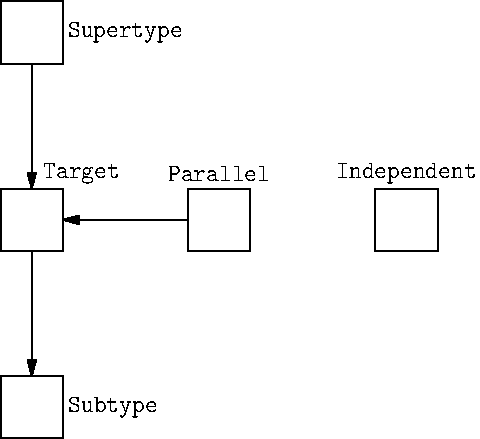
\includegraphics[width=0.5\textwidth]{typedef}
\caption{Typedef relationships}
\label{fig:typedef}
\end{figure}

\begin{description}
\item[subtype:] That's the standard subclass or \D{alias this} relationship: a subtype can act \emph{in lieu of} its parent type in all circumstances. Whatever its parent can do, the subtype does also. Moreover, the subtype can be forcibly cast as its parent type (think classes).
\item[supertype:] The converse: a supertype can be assigned a value of type 'target', its subtype (since a subtype can act as its supertype), and that's about it. Once the supertype and functions acting on it are created, the original target type can be used there also.
\item[parallel:] A parallel type is neither a subtype not a supertype of the original target (it cannot mimic the target), but it can be created with target values. It's more or less the behaviour of the now-deceased \D{typedef} keyword.
\item[independent:] An independent type is just there and bears no relationship whatsoever with the original, target type. I cite it there but the interest of defining such a type while still having a 'target' type in mind is limited\ldots
\end{description}

Here is clean little piece of code from Trass3r that groups all these notions in one template:

\begin{dcode}
module librarytypedef;

enum Relationship
{
    Independent,
    Super,
    Sub,
    Parallel,
}

struct Typedef( Target, 
                Relationship relation = Relationship.Sub, 
                Target init = Target.init, 
                string _f = __FILE__,
                int _l = __LINE__ )
{
    Target payload = init;

    static if ( relation != Relationship.Independent )
        this( Target value )
        {
            payload = value;
        }

    static if ( relation == Relationship.Sub)
        // typedef int foo; foo f;
        // f.opCast!(t)() == cast(t) f
        Target opCast(Target)()
        {
            return payload;
        }

    static if ( relation == Relationship.Sub 
             || relation == Relationship.Parallel )
        alias payload this;

    static if ( relation == Relationship.Super )
        typeof( this ) opAssign( Target value )
        {
            payload = value;
            return this;
        }
    else static if ( relation == Relationship.Sub )
        @disable void opAssign( Target value );
}
\end{dcode}

\TODO{Give some examples.}

\section{Types as Information}
\label{typesasinformation}

\subsection{User-Defined Literals}\label{userdefinedliterals}

In \href{http://drdobbs.com/blogs/tools/229401068}{this article}, Walter Bright makes a convincing case for using templates as user-defined literals. His example is now the \stdanchor{conv}{octal} wrapper that allowed D to (see if it's possible to) ditch octal literals as a compiler construct and push them into library-space. That way, you can use:

\begin{dcode}
auto o1 = octal!"755";
// or even:
auto o2 = octal!755;
\end{dcode}

as a stand-in replacement for the \DD{0755} octal literal. It's no more complicated to type (a few chars to add at most), it's clearer for a reader of your code (who may miss the beginning \DD{0}) that he's dealing with an octal there. Best of all, the implementation is there as library code: easy to reach, easy to debug\footnote{ And less intimidating than diving into compiler code.} and easy to duplicate for other encodings. That way, this could be done:

\begin{dcode}
auto h1 = hexa!"deadbeef";
auto b1 = binary!1011011;
// Or even:
auto number = base!(36, "4d6r7th2h7y");
\end{dcode}

Behind the scene, \DD{octal} reads its \D{string} or \D{int} argument and converts it into an \D{int} or a \D{long} depending on the argument size.  It's a nice piece of work that could pave the way to similar well-integrated language extensions.

\unfinished{Also, DSL in strings in D, see Statically-Checked Writeln in \ref{staticallycheckedwriteln}, encoding informations in types (\ref{encodinginformationwithtypes}) and annotating types (\ref{annotatingtypes}).}


\subsection{Encoding Information With Types}
\label{encodinginformationwithtypes}

This is an extension of the previous section's idea, that can be found for example in \stdanchor{range}{assumeSorted} and \stdanchor{range}{SortedRange}. These Phobos constructs encode some information in a type (in this case, the fact than the range is sorted, with an associated predicate). That way, subsequent operations acting on a range can use better algorithm if they know it's sorted.

This kind of encoding can be used for many different schemes:

\begin{itemize}
\item For a matrix library, you could have a, for example, \DD{assumeHermitian} or \DD{assumeTriangular} that just wraps a pre-existing matrix.
\item For a XML/HTML library, you could imagine a \DD{Validated} struct that's used to indicate, er, validated content. Any external input will have to pass trough a \DD{validate} function that delivers the \DD{Validated} object. Subsequent operations will work only on \DD{Validated} data, not raw data.
\item A units library (as in, $kg.m/s^{2}$, not unit-testing) is mainly a bunch of \D{double} (or complex) values wrapped in a multi-checked type that allows only some operations, depending on types. \DD{meter(5) + kilo(gram(10))} is a no-no, but \DD{meter(5)*kilo(gram(10))} is OK.
\end{itemize}

Moreover, it's easy to provide additional information:

\begin{dcode}
struct MinMax(T)
{
    T min;
    T max;
    
    T value;
    
    alias value this;
}
\end{dcode}

In this case, \DD{MinMax} means the wrapped value is between \DD{min} and \DD{max} (the enforcing code would be in the factory function, for example).
        
Things get interesting when using multiple wrappers inside one another. Imagine we have three wrappers, for numerical ranges with an ordering operation:

\begin{itemize}
\item \DD{minmaxed}, which ascertains (well, at least transmits the message) that the wrapped value is between to extrema.
\item \DD{periodic}, which encodes the idea the range has a period, accessible through the \DD{.period} member.
\item \DD{derivative}, which says successive elements' difference is no more than a \DD{.slope} number (in absolute).
\end{itemize}

\begin{dcode}
import std.range: cycle;

auto range = cycle([0,1,2,3,4,3,2,1]);
auto withMetadata = minmaxed( 
                              periodic( 
                                       derivative( range
                                                 , 1)
                                      , 8
                            , 0, 10);

assert(withMetadata.period == 8); // propagated all the way up.
\end{dcode}

So, in the previous sample, \DD{withMetadata}'s elements are at the same time limited in variation, limited in value and periodic. The trouble is when we want to shift metadata around, comparing types with metadata ordered in a different way: obviously for us humans, a range with suprema and periodic is \emph{also} periodic and with suprema. But as far as D is concerned a \DD{minmaxed(periodic())} and a \DD{periodic(minmaxed())} do not have the same type. For more on this notion, see section \ref{annotatingtypes} on annotating types.

\TODO{A unit example in the Examples part? It may be a bit big\ldots}

\section{Templates in Templates}\label{templatesintemplates}

Sometimes, you know users of your code will send to your template a first list (of indefinite length) of parameters, followed by a second list. Seeing that, you may want to write code like the following:

\begin{dcode}
template MyTemp(A..., B...)
{ ... }
\end{dcode}

Halas, two template parameters tuples do not make sense (see \autoref{declarations}). But it's not a dead-end. First, you could try to write:

\begin{dcode}
template(AB...)
{ ... }
\end{dcode}

And filter the \DD{AB}s to find the ones you need. It can be done by \DD{staticFilter}, presented in \ref{staticfilter} (and its associated function on a function arguments would be \DD{tupleFilter} shown in \ref{filteringtuples}). In this case, the two series of arguments can be completely mixed (and not separated in two lists), which is strictly more powerful. On the other hand, it means you must be able to separate them by their types alone, which may not be possible.

\subsection{Templates All the Way Down}

Happily, the initial problem can easily be solved this way:

\begin{dcode}
template MyTemp(A...)
{
    template MyTemp(B...)
    {
    (...)
    }
}
\end{dcode}

Remember, a template can have template members. So you can nest templates within templates, each with its own constraints and intermediate code. If you use the same name through and through the eponymous trick will be activated, but sometimes using a different name at each stage can make your code more readable.

For example, what if you want to compare to template tuples to see if they contain the same arguments?

\begin{dcode}
module compare;

template Compare(First...)
{
    template With(Second...)
    {
        static if (First.length != Second.length)
            enum With = false;
        else static if (First.length == 0) // End of comparison
            enum With = true;
        else static if (!is(First[0] == Second[0]))
            enum With = false;
        else
            enum With = Compare!(First[1..$]).With!(Second[1..$]);
    }
}

//Usage:
unittest
{
    alias Compare!(int, double, string).With!(int, double, char) C;
    static assert(C == false);
}
\end{dcode}

In that case, using \DD{With} inside \DD{Compare} let the code be quite easy to use. Notice that the eponymous trick is done only on \DD{With}, because it's this inner template that we want the result of.

Going back to \DD{MyTemp}, using it is slightly more complicated:

\begin{ndcode}
// Yes:
alias MyTemp!(int, double, string) MyTemp1;
MyTemp1!(char, void);

// No:
MyTemp!(int, double, string)!(char, void);
// No :
MyTemp!(int, double, string).!(char, void);
\end{ndcode}

The D grammar does not authorize multiple template calls like the ones on lines 6 and 8. You must use an alias for the intermediate stage. It's not that drastic a limitation, because if you created the template as a multi-step construction, it's most probably because you wanted to do a multi-step invocation\ldots

\subsection{Double-Stage Function Templates}

For function templates, this can give very powerful things. You can have a place in your code where compile-time parameters are given, which delivers another, crafted-just-for-your-needs, template which you can instantiate later on. See for example \ref{stringinterpolation} and the \DD{interpolate} function-in-template.

Policies are particularly good with this idiom.\index{idiom!functions in templates} Section \ref{memoizing} presents a template that transforms a standard D function into a memoized one. Here is what could be done if it was a two-steps template:

\begin{dcode}
/*
 * memoizer will store the first million tuple of args
 * and discard half of them when the maximum is reached, 
 * to free some memory. At this stage, the function it 
 * will memoize is not known. The user decided this
 * particular instantiation was the best memoizing 
 * strategy in her code. memoizer could (and will!) be 
 * applied on many different functions.
 */
alias memoize!(Storing.maximum, 1_000_000, Discarding.fraction, 0.5f) memoizer;

auto longCalculation1(int i, double d) { ... }
auto longCalculation2(double d, string s) { ... }

/*
 * longCalculation1 and longCalculation2 will both profit 
 * from the memoization even though they have different 
 * signatures, different arguments and return a different type.
 */
alias memoizer!longCalculation1 mlc1;
alias memoizer!longCalculation2 mlc2;
\end{dcode}

\TODO{OK, now maybe I should provide an updated version of \DD{memoize} in \ref{memoizing}.}

\subsection{Named-Fields Tuples}\label{namedfieldstuples}

Let's have another example, to use IFTI (\ref{ifti}). In Phobos, the function \stdanchor{typecons}{tuple} lets you create a tuple on the fly. It's a very nice example of IFTI in action:

\begin{dcode}
module usingtuple;
import std.typecons;

void main()
{
    auto tuple1 = tuple(1, 3.14159, "abc"); // tuple1 is a Tuple!(int,double,string)
    auto tuple2 = tuple('a','b','c');       // tuple2 is a Tuple!(char,char,char)
}
\end{dcode}

But Phobos' \DD{Tuple} is more powerful than that. It can have named parameters:

\begin{dcode}
Tuple!(int, "counter", string, "name") myCounter;
myCounter.counter = -1;
myCounter.name = "The One and Only Counter Around There";
\end{dcode}

As of this writing, Phobos doesn't provide a \DD{tuple} factory function allowing named arguments in an nice, automated manner:

\begin{dcode}
module usingnamedtuple;
import namedtuple;

void main()
{
    auto myCounter = tuple!("counter", "name")(-1, "Who's his Daddy's counter?");

    myCounter.counter = 1;

    // Or even:
    alias tuple!("counter", "name") makeCounter;

    auto c1 = makeCounter(0, "I count ints!");
    auto c2 = makeCounter("Hello", "I'm a strange one, using strings");

    c2.counter ~= " World!"; 
}
\end{dcode}

In the previous example, \DD{c1} is a \DD{Tuple!(}\D{int}\DD{,}\D{string}\DD{)}, whereas \DD{c2} is a \DD{Tuple!(}\D{string}\DD{,}\D{string}\DD{)}. That means \DD{makeCounter} is a factory function for tuples with two fields, named \DD{counter} and \DD{name}, which see their types determined later on. I want this, so let's code it.

First, it's obvious we need a two-stage template:

\index{template!constraints}
\begin{dcode}
import std.typetuple: allSatisfy;

template tuple(names...) 
if (names.length && allSatisfy!(isAStringLiteral, names))
{
    auto tuple(T...)(T args)
    {
    (...)
    }
}
\end{dcode}

The constraint is here to check that the user gives at least one name and also that all passed \DD{names} are indeed string literals template parameters. I use \stdanchor{typetuple}{allSatisfy} to verify the condition on all of them. I cannot use directly \stdanchor{traits}{isSomeString} because this template acts on types, whereas I need something checking a string literal.

\begin{dcode}
module isastringliteral;
import std.traits: isSomeString;

template isAStringLiteral(alias name)
{
    enum isAStringLiteral = isSomeString!(typeof(name));
}
\end{dcode}

That being in place, we need to create the correct \DD{Tuple}. Arguments names are provided right after each type (so as to allow for a mix between named and anonymous fields:

\begin{dcode}
/*
 * The first two fields are named, and the fourth.
 * The third is anonymous.
 */
alias Tuple!(int, "counter", string, "name", double, double, "total") MyTuple;
\end{dcode}

For our function, we consider that, given $n$ names, the first $n$ arguments will be named and the remaining (if any) will be anonymous. That give us another constraint: if the user provide less than $n$ arguments, we refuse the input and stop the compilation right there.

\index{template!constraints}
\begin{dcode}
import std.typetuple: allSatisfy;

template tuple(names...) 
if (names.length && allSatisfy!(isAStringLiteral, names))
{
    auto tuple(T...)(T args) if (T.length >= names.length)
    {
    (...)
    }
}
\end{dcode}

Now, we just need the alternate the names and the argument types. Happily, this document describe a \DD{Interleave} template in \ref{interleavingtypes}, that does just that:

\begin{dcode}
module namedtuple;
import std.typecons;
import std.typetuple;
import interleave;
import isastringliteral;

template tuple(names...) 
if (names.length && allSatisfy!(isAStringLiteral, names))
{
    auto tuple(T...)(T args) if (T.length >= names.length)
    {
        return Tuple!(Interleave!(T).With!(names))(args);
    }
}
\end{dcode}

And, presto, here we have our named-tuple factory function. Isn't that nice? The closure example in \ref{closuresareapoormansobjects} could use it to simplify its returned value.

\TODO{And a curried template.}

\section{\texorpdfstring{\D{\_\_FILE\_\_} and \D{\_\_LINE\_\_}}
                        {\_\_FILE\_\_ and \_\_LINE\_\_}}
\label{fileandline}

\unfinished{This section needs some heavy testing. My D config was broken when I wrote this part. Take everything in there with a \emph{big} grain of salt. It's on my todo list to test and rewrite everything.}

In section \ref{default}, we've seen that template parameters can have default values. There are also two special, reserved, symbols that are defined in D: \D{\_\_FILE\_\_} and \D{\_\_LINE\_\_}. They are used in standard (non-\D{mixin}) templates, but their behaviour will remind you of mixins: when instantiated, they get replaced by strings containing the file name and the line in the file of the \emph{instantiation call site}. Yes, it's a sort of two-way dialogue: module \DD{a.d} defines template \DD{T}. Module \DD{b.d} asks for a \DD{T} instantiation. This instantiation is done in module \DD{a.d}, but will line and filename taken from \DD{b.d}!

They are mostly declared like this:

\index{\_\_FILE\_\_ and \_\_LINE\_\_@\D{\_\_FILE\_\_} and \D{\_\_LINE\_\_}!unique types}
\begin{dcode}
module filelinetagging;

struct Unique(T, string file, size_t line)
{
    enum size_t l = line;
    enum string f = file;
    T t;
}

auto unique(T, string file = __FILE__, size_t line = __LINE__)(T t)
{
    return Unique!(T, file, line)(t);
}
\end{dcode}

As \DD{Unique}'s name suggests, this is a way to obtain unique instantiations. Except if you call the very same template twice in the same line of your file, this pretty much guarantee your instantiation will be the only one. Remember that template arguments become part of the template scope\index{scope!template scope} name when instantiation is done (\ref{instantiating}).

\begin{dcode}
module usingunique;
import filelinetagging;

void main()
{
    auto u = unique(1); // Unique!(int, "thefile.d", 4)

    auto v = unique(1); // Unique!(int, "thefile.d", 6)

    static assert(!is( typeof(v) == typeof(u) ));
}
\end{dcode}

Even though \DD{u} and \DD{v} are declared the same way, they have different types.

Apart from \emph{one-of-a-kind} types, this is also useful for debugging: you can use the strings in error messages:

\index{\_\_FILE\_\_ and \_\_LINE\_\_@\D{\_\_FILE\_\_} and \D{\_\_LINE\_\_}!debugging}
\begin{dcode}
auto flatten(Range, file == __FILE__, line == __LINE__)(Range range)
{ 
    static if (rank!Range == 0)
        static assert(0, "File: " ~ file ~ " at line: " ~ line 
                       ~ ", flatten called with a rank-0 type: " 
                       ~ Range.stringof);
    else static if (rank!Range == 1)
        return range;
    else
        return Flatten!(Range)(range);
}
\end{dcode}

And here is a little gift:

\begin{dcode}
module debugger;

/** Usage:
 * Debug!(templateToBeTested).With!(Argument0, Argument1, Argument2);
 */
template Debug(alias toTest, string file = __FILE__, size_t line = __LINE__)
{
    template With(Args...)
    {
        static if (is( toTest!Args ))
            alias toTest!Args With;
        else
            static assert(0, "Error: " ~ to!string(toTest)
                           ~ " called withs arguments: "
                           ~ Args.stringof);
    }
}
\end{dcode}

That way, no need to modify your beautiful templates.

\TODO{Test that.}



\newpage
\part{Examples}\label{examples}

This part will present various examples showing what can be done with D templates, be it type manipulation, code generation or language extension \ldots Most examples are code snippets that were useful to me at one time or another. I hope they will be useful to you too.

\aparte{Contributors welcome!}{Even more than for other parts, I welcome any short and synthetic example of what can be done with templates. Do not hesitate to chime in and push some code in this doc!}

\section{Type Sorcery}\label{typesorcery}

One of the most fundamental use of templates is type sorcery: type creation, type manipulation, etc. D being a statically type language, all of your creations will have a defined type. Sometimes, these can be cumbersome to write or manipulate. Templates can help you in this.

\subsection{Mapping, Filtering and Folding Types}

As we saw in section \ref{tuples}, template tuple parameters can hold type tuples (that's even their original role). Since these can be iterated, indexed or sliced, they are ideal candidates to some standard iteration algorithms. As for ranges, you can map another template on type tuples, filter the types you want to extract or fold (reduce) them into another type.

\aparte{And non-types?}{What about acting on expression tuples? You can do that too. Even though this section is called \emph{Type} Sorcery, all templates here can work on expression tuples too. Do not feel limited.}

\subsubsection{Mapping on Type Tuples}\label{staticmap}

Mapping a type tuple is simply applying another (unary) template on all types of a type tuple. Phobos already defines \DD{staticMap} in \std{typetuple}, but it's a nice exercise to code it again. We want a template that takes another template name (as an \D{alias} parameter), say \DD{Wrapper}, and a typetuple (\DD{T0, T1, T2, ..., Tn}) and returns \DD{Wrapper!T0, Wrapper!T1, Wrapper!T2, ..., Wrapper!Tn}.

\begin{dcode}
template staticMap(alias M, T...)
{
    static if (T.length == 0) // End of sequence
        alias TypeTuple!() staticMap; // stop there
    else
        alias TypeTuple!(M!(T[0]), staticMap!(M, T[1..$])) staticMap;
}
\end{dcode}

We use the auto-flattening of type tuples to aggregate the results into a unique tuple. Notice how indexing and slicing make for a not-so-complicated piece of code.

Even a simple template such as this one can have great uses:

\begin{itemize}
\item Getting rid of all qualifiers in a type list, by mapping \stdanchor{traits}{Unqual} on the types.
\item Generating a huge quantity of types by using a typetuple-returning mapper (see below).
\item Given a bunch of function types, getting their return types or parameter typetuples.
\end{itemize}

\subsubsection{Example: Testing a Function}

The seconde use in the previous section's list can be useful to unit-test a part of your code. Suppose you have a templated function that is supposed to work on any built-in type. You do not need to generate all possible combinations of types. Just use \DD{staticMap} to generate them for you:

\begin{dcode}
/** 
* Given a type T, generates all qualified versions of T
* that you find interesting (eleven versions all in all).
*/
template Qualified(T)
{
    alias TypeTuple!(
                     T, const(T), immutable(T), shared(T),
                     T[],const(T)[],immutable(T)[], shared(T)[], 
                     const(T[]), immutable(T[]), shared(T[])
                    ) Qualified;
}

// All 16 built-in types you're interested in.
alias TypeTuple!(
                 bool,
                 ubyte,byte,
                 ushort,short,
                 uint,int,
                 ulong,long,
                 float,double,real,
                 char,wchar,dchar
                ) ValueTypes;

// Bang, 11*16 types generated.
alias staticMap!(Qualified,ValueTypes) QualifiedTypes;

// If you're really a pervert (note that there will be duplicates)
alias staticMap!(Qualified, QualifiedTypes) DoublyQualifiedTypes;
\end{dcode}

Now, if your function is supposed to work on all the generated qualified types, just test it:

\begin{dcode}
void myFun(T)(T t) { ... }

/* Here we generate the qualified types, see above */
(...) 
temp
late test(alias fun)
{
    void on(T...)()
    {
        foreach(Type; T)
            static if (!__traits(compiles, fun(Type.init)))
                pragma(msg, "Bad testing combination: " 
                          ~ fun.stringof ~ " and " ~ Type.stringof);
    }
}
   
unittest 
{
    test!(myFun).on!(QualifiedTypes);
}
\end{dcode}

\subsubsection{Filtering Type Tuples}\label{staticfilter}

You can search for and extract some types from a tuple, using a predicate to chose which type (or more generally, which tuple element) you want to keep. A predicate in this particular case means 'a template that, when given a type as argument, will return either \D{true} or \D{false}'. The test done on the tuple element can be as complicated as you want, particularly using \D{is}\DD{()} expressions (see \autoref{isexpression}).

That gives us the following code:

\begin{dcode}
template staticFilter(alias Pred, T...)
{
    static if (T.length == 0) // End of sequence
        alias TypeTuple!() staticFilter;
    else static if (Pred!(T[0])
        alias TypeTuple!(T[0], staticFilter!(Pred, T[1..$])) staticFilter;
    else
        alias TypeTuple!(      staticFilter!(Pred, T[1..$])) staticFilter;
}
\end{dcode}

Using \DD{staticFilter} is quite simple. Let's get integral types from a tuple, by way of \stdanchor{traits}{isIntegral}:

\begin{dcode}
alias TypeTuple!(int, double, float, string, byte, bool, float, void) Types;

alias staticFilter!(isIntegral, Types) OnlyIntegrals;

static assert(is(OnlyIntegrals == TypeTuple!(int, byte, bool)));
\end{dcode}

But that is, admittedly, pretty boring stuff. Though useful from time to time, it's quite rare for someone to be given a pure type tuple like this. A much more common use for the likes of \DD{staticFilter} is when creating complex types.

\subsubsection{Example: building a \DD{Graph}}

As a first example, imagine you have a \DD{Graph(Node, Edge)} struct, templated on the nodes (vertice) and edges types (themselves templated). When you create a \DD{Graph} with a factory function (\ref{factory}), it would be nice to be able to mix nodes and edges in a natural way. That is, given \DD{graph}, \DD{node} and \DD{edge} functions that do the obvious thing, you want to autorize calls like:

\begin{dcode}
/** 
* Automatically creates a graph 
*   - with four nodes labelled "A", "B", "C", "D", holding a double, 
*   - with nodes linking "A" to "B", "D" to "A" and "D" to "C".
*/
auto g = graph(node("A", 3.14159), node("B", 1.0), 
               edge("A","B"),
               node("C", 2.71828), node("D", 0.0), 
               edge("D","A"), edge("D", "C"));
\end{dcode}

This allows the user building her \DD{Graph} to create nodes and edges between these nodes in a natural way (as opposed to, say, batch-building all nodes and then adding edges between them). But, as a library writer, that means your \DD{graph} factory function has the following signature:

\begin{dcode}
auto graph(NodesOrEdges...)(NodesOrEdges args) 
if (/* sanity check test on NodesOrEdges */)
\end{dcode}

Both the sanity check performed by the template constraint (\ref{constraints}) and the building code inside \DD{graph} can be quite complicated. \DD{staticFilter} helps by separating the arguments between nodes and edges. Without extending this example too much, say we have at our disposal the following predicate templates:

\begin{dcode}
template isNode(N) {/* true iff N is a Node!(LabelType, ValueType)*/}
template isEdge(E) {/* true iff E is an Edge!(LabelType)*/}

template isNodeOrEdge(T)
{
    static if (isNode!T || isEdge!T)
        enum isNodeOrEdge = true;
    else
        enum isNodeOrEdge = false;
}
\end{dcode}

And let's suppose also all \emph{bona fide} \DD{Node}s and \DD{Edge}s have  \DD{.LabelType} and \DD{.ValueType} members exposing their inner types (as shown in \autoref{inneralias}).

Then, getting all nodes and edges is easy:
\begin{dcode}
alias staticFilter!(isNode, NodesOrEdges) Nodes;
alias staticFilter!(isEdge, NodesOrEdges) Edges;
\end{dcode}

This is where things get interesting: obtaining the edges and nodes types is just a first building block. Now \DD{graph} must check at a minimum the following elements:

\begin{enumerate}
\item All arguments must be nodes or edges.
\item Is there at least \emph{one} node in the list?
\item If yes, do all nodes have the same \DD{LabelType} and the same \DD{ValueType}, or, at least, is there a common type between all the labels' types and another one for the values stored in the nodes?
\item Do edges' \DD{LabelTypes} have a common type? (Note that there can be zero edges).
\item Do the edges labels have the correct type to refer to the provided nodes?
\end{enumerate}

Note that \emph{all} these checks are done only on types and thus can be done at compile-time, thereby ensuring a pretty solid static check on the graph built. What cannot be done in this way is verifying during compilation that edges do indeed refer to existing nodes.

Let's use what we have seen until now to create the \DD{GraphCheck}\label{graphcheck} template, before seeing another \DD{staticFilter} example:

\begin{dcode}
import std.traits: CommonType;

template GraphCheck(NodesOrEdges...)
{
    enum GraphCheck = GraphCheckImpl!(NodesOrEdges).result;
}

template GraphCheckImpl(NodesOrEdges...)
{
    alias staticFilter!(isNode, NodesOrEdges) Nodes;
    alias staticFilter!(isEdge, NodesOrEdges) Edges;
    
    // 1. All arguments must be nodes or edges
    static if (Nodes.length + Edges.length != NodesOrEdges.length)
    static assert(0, "Some args are not nodes or edges.");
    
    // 2. There must be at least one node
    static if (Nodes.length == 0)
    static assert(0, "You must provide at least one node.");
    
    // 3. Is there a common type for the nodes' labels and values?
    // First step: extracting labels and values
    template GetLabel(T) if (isNode!T || isEdge!T)
    {
        alias T.LabelType GetLabel;
    }
    
    template GetValue(T) if (isNode!T)
    {
        alias T.ValueType GetValue;
    }

    alias staticMap!(GetLabel, Nodes) NodesLabels;
    alias staticMap!(GetValue, Nodes) NodesValues; 
    
    static if (is(CommonType!(NodesLabels) == void)) // no common type
    static assert(0, "The nodes do not have all the same label type.");
    
    static if (is(CommonType!(NodesValues) == void))
    static assert(0, "The nodes do not have all the same value type.");

    // 4. Same for edges
    alias staticMap!(GetLabel, Edges) EdgesLabels;  
    
    static if (is(CommonType!(EdgesLabels) == void))
    static assert(0, "The edges do not have all the same label type.");
        
    // 5. Edges - Node compatibility
    static if(!is(CommonType!NodesLabels == CommonType!EdgesLabels))
        static assert(0, "Nodes and edges do not have the same label type.");
    
    enum result = true;
}    
\end{dcode}

This is one huge template, but \DD{staticFilter} sits square in the middle and greatly simplifies the code. Now, \DD{graph} signature is simply:

\begin{dcode}
auto graph(NodesOrEdges...)(NodesOrEdges args) if (GraphCheck!NodesOrEdges)
{ ... }
\end{dcode}

\unfinished{The second example will be one code generating a struct, with string literal and type parameters.}

\subsubsection{Folding Type Tuples}\label{staticreduce}

\TODO{Examples to give: biggest type in the lot, sorting types?}

\subsection{Zipping Types, Interleaving Types, Crossing Types}

\TODO{Determine if this subsection is really useful. Is there any short and telling example?}

\subsubsection{Interleaving Types}\label{interleavingtypes}

\begin{dcode}
/**
 * Given (T0, T1, T2, ..., Tn) and (U0, U1, ..., Um) will returns
 * the interleaving of the first part with the second part: 
 *
 * (T0, U0, T1, U1, ...
 *
 * If one of the inputs is shorter than the other, 
 * the longer part is put at the end of the interleaving.
 */
template Interleave(First...)
{
    template With(Second...)
    {
	static if (First.length == 0)
	    alias Second With;
	else static if (Second.length == 0)
	    alias First With;
	else
	    alias TypeTuple!( First[0], Second[0]
	                    , Interleave!(First[1..$]).With!(Second[1..$])) 
             With;
    }
}

\end{dcode}

\section{Tuples as Sequences}\label{tuplesassequences}

\subsection{Mapping on Tuples}\label{mappingontuples}

\subsection{Filtering Tuples}\label{filteringtuples}

\begin{dcode}
(1, "abc", 2, "def", 3.14)
->
((1,2),("abc","def"),(3,14))
\end{dcode}


\section{Fun With Functions}\label{funwithfunctions}

This section will present some templated wrappers around functions, to provide some additional usefulness. It's not part of \autoref{functiontemplates} because it uses struct templates and it's not part of \autoref{structtemplates} because the wrapper struct is not the main focus of attention.

\subsection{Memoizing a Function} \label{memoizing}

When a function does long calculations, it might be efficient to store the computed results in an external structure and to query this structure for the result instead of calling the function again. This is called \emph{memoizing} (not \emph{memorizing}\ldots) and this sectino will show how to use a template to have some memoizing fun.

The previously-seen results are stored in an associative array, indexed on tuples of arguments. To get a function return type or parameter type tuple, just use Phobos' \stdanchor{traits}{ReturnType} and \stdanchor{traits}{ParameterTypeTuple}, which are templates that accept function \emph{names} or types.

\index{struct template!memoize@\DD{memoize}}
\index{function templates!wrapping a function!memoize@\DD{memoize}}
\index{template!parameters!alias}
\begin{dcode}
struct Memoize(alias fun)
{
    alias ReturnType!fun RT;
    alias ParameterTypeTuple!fun PTT;
    RT[Tuple!(PTT)] memo; // stores the result, indexed by arguments.

    RT opCall(PTT args)
    {
        if (tuple(args) in memo)      // Have we already seen these args?
        {
            return memo[tuple(args)]; // if yes, use the stored result
        }
        else // if not, compute the result and store it.
        {
            RT result = fun(args);
            memo[tuple(args)] == result;
            return result;
        }
    }
}

Memoize!fun memoize(alias fun)()
{
    return Memoize!fun();
}
\end{dcode}

Usage is very simple:

\begin{dcode}
int veryLongCalc(int i double d, string s) { ... }

auto vlcMemo = memoize!(veryLongCalc);

// calculate veryLongCalc(1, 3.14, "abc")
// takes minutes!
int res1 = vlcMemo(1, 3.14, "abc"); 
int res2 = vlcMemo(2, 2.718, "def");// minutes again!
int res3 = vlcMemo(1, 3.14, "abc"); // a few ms to get res3
\end{dcode}

The above code is trivial and could be optimized in many ways. Mostly, a real memoizing template should also modify its behavior with storing policies. For example:

\begin{itemize}
\item No-limit or limited size store? 
\item In case of limited-size store: how to define the limit and what should be the eviction policy?
\begin{itemize}
\item First-in/First-out memo?
\item Least recenly used memo?
\item Least used?
\item Time-to-live?
\item Discard all and flush the store?
\item Discard only a fraction?
\item Stop memoizing?
\end{itemize}
\end{itemize}

The last X results could be stored in a queue: each time a result is pushed into the associative array, push the arguments tuples in the queue. Once you reach the maximum store limit, discard the oldest one or (for example) half the stored values.

Here is a possible small implementation. It makes for a nice example of enabling/disabling code with \D{static if} and \D{enum}-based policies. Note that I use D dynamic arrays as a primitive queue. A real queue could probably be more efficient, but there isn't one in the standard library as of this writing.

\index{struct template!memoize@\DD{memoize}}
\index{function templates!wrapping a function!memoize@\DD{memoize}}
\index{template!parameters!alias}
\index{enabling/disabling code}
\index{enum-based policy@\D{enum}-based policy}
\index{idiom!enabling/disabling code}
\index{idiom!policy}
\begin{dcode}
enum Storing { 
    always,  // there is no tomorrow
    maximum  // sustainable growth
}

enum Discarding { 
    oldest,   // only discard the oldest result
    fraction, // discard a fraction (0.5 == 50%)
    all       // burn, burn!
}

struct Memoize(alias fun, 
               Storing storing,
               Discarding discarding)
{
    alias ReturnType!fun RT;
    alias ParameterTypeTuple!fun PTT;

    static if (storing == Storing.maximum)
    {
        Tuple!(PTT)[] argsQueue;
        size_t maxNumStored;
    }
    
    static if (discarding == Discarding.fraction)
        float fraction;

    RT[Tuple!(PTT)] memo; // stores the result, indexed by arguments.
    
    RT opCall(PTT args) 
    {
        if (tuple(args) in memo)      // Have we already seen these args?
        {
            return memo[tuple(args)]; // if yes, use the stored result
        }
        else                          // if not,
        {                             
            static if (storing == Storing.always)
            {
                RT result = fun(args);// compute the result and store it.
                memo[tuple(args)] = result;
                return result;
            }
            else // Storing.maximum
            {
                if (argsQueue.length >= maxNumStored)
                {
                    static if (discarding == Discarding.oldest)
                    {
                        memo.remove(argsQueue[0]);
                        argsQueue = argsQueue[1..$];
                        writeln("Discarding oldest.");
                    }
                    else static if (discarding == Discarding.fraction)
                    {
                        auto num = to!size_t(argsQueue.length * fraction);
                        foreach(elem; argsQueue[0..num])
                            memo.remove(elem);
                        argsQueue = argsQueue[num..$];
                        writeln("Discarding fraction.");
                    }
                    else static if (discarding == Discarding.all)
                    {
                        memo = null;
                        argsQueue.length = 0;
                        writeln("Discarding all.");
                    }
                }
                
                RT result = fun(args);// compute the result and store it.
                memo[tuple(args)] = result;
                argsQueue ~= tuple(args);
                return result;            
            }
        }
    }
}
\end{dcode}

And a few factory function to help creating those \DD{Memoize} structs:

\begin{dcode}
// No runtime arg -> always store
Memoize!(fun, Storing.always, Discarding.all)
memoize(alias fun)()
{
    Memoize!(fun, 
             Storing.always, 
             Discarding.all) result;
    return result;
}

// One runtime size_t arg -> maximum store / discarding all
Memoize!(fun, Storing.maximum, Discarding.all)
memoize(alias fun)(size_t max)
{
    Memoize!(fun, 
             Storing.maximum, 
             Discarding.all) result;
    result.maxNumStored = max;
    return result;
}

// Two runtime args (size_t, double) -> maximum store / discarding a fraction
Memoize!(fun, Storing.maximum, Discarding.fraction)
memoize(alias fun)(size_t max, double fraction)
{
    Memoize!(fun, 
             Storing.maximum, 
             Discarding.fraction) result;
    result.maxNumStored = max;
    result.fraction = fraction;
    return result;
}

// One compile-time argument (discarding oldest), one runtime argument (max)
Memoize!(fun, Storing.maximum, discarding)
memoize(alias fun, Discarding discarding = Discarding.oldest)
(size_t max)
{
    Memoize!(fun, 
             Storing.maximum, 
             Discarding.oldest) result;
    result.maxNumStored = max;
    return result;
}
\end{dcode}

Note that, due to the introduction of an \DD{opCall} operator, it's not possible to use a struct literal. We have to first create the struct, then initialize its fields.

Most of the time, the type of runtime arguments is enough to determine what you want as a memoizing/storing behavior. Only for the (rarer?) policy of discarding only the oldest stored result does the user need to indicate it with a template argument:

\begin{dcode}
int veryLongCalc(int i double d, string s) { ... }

// Store the first million results, flush the memo on max
auto vlcMemo1 = memoize!(veryLongCalc)(1_000_000);

// Store the first million results, flush half the memo on max
auto vlcMemo2 = memoize!(veryLongCalc)(1_000_000, 0.5f);

// Store first twenty results, discard only the oldest
auto vlcMemo3 = memoize!(veryLongCalc, Discarding.oldest)(20);
\end{dcode}

\subsection{Currying a Function} \label{currying}

\unfinished{Some explanations would greatly help there.}

Another useful transform on functions is to \emph{curry}\footnote{from Haskell Curry, the guy who formalized the idea.} them: to transform a $n$-args function into $n$ one-parameter functions inside another.

\TODO{Show some example: mapping a range for example.}

\index{static if@\D{static if}!recursion}
\index{static if@\D{static if}!nested}
\index{template!double-decker template!CheckCompatibility.With@\DD{CheckCompatibility.With}}
\begin{dcode}
template CheckCompatibility(T...)
{
    template With(U...)
    {
        static if (U.length != T.length)
            enum With = false;
        else static if  (T.length == 0) // U.length == 0 also
            enum With = true;
        else static if (!is(U[0] : T[0]))
            enum With = false;
        else
            enum With = CheckCompatibility!(T[1..$]).With!(U[1..$]);
    }
}
\end{dcode}

\index{operator!opCall, ()@\DD{opCall}, \DD{()}}
\index{template!parameters!integral value}
\index{template!parameters!alias}
\index{static assert@\D{static assert}}
\begin{dcode}
struct Curry(alias fun, int index = 0)
{
    alias ReturnType!fun RT;
    alias ParameterTypeTuple!fun PTT;
    PTT args;

    auto opCall(V...)(V values)
        if (V.length > 0
         && V.length + index <= PTT.length)
    {
        // Is fun directly callable with the provided arguments?
        static if (__traits(compiles, fun(args[0..index], values)))
            return fun(args[0..index], values);
        // If not, the new args will be stored. We check their types.
        else static if (!CheckCompatibility!(PTT[index..index + V.length]).With!(V))
            static assert(0, "curry: bad arguments. Waited for "
                            ~ PTT[index..index + V.length].stringof
                            ~ " but got " ~ V.stringof);
        // not enough args yet. We store them.
        else
        {
            Curry!(fun, index+V.length) c;
            foreach(i,a; args[0..index]) c.args[i] = a;
            foreach(i,v; values) c.args[index+i] = v;
            return c;
        }
    }
}

auto curry(alias fun)()
{
    Curry!(fun,0) c;
    return c;
}
\end{dcode}

\subsection{Juxtaposing functions}\label{juxtapose}

\TODO{See where the code is. It used heavy-duty type manipulation IIRC.}

\section{Relational Algebra}

Inspiration for this example comes from \href{http://david.rothlis.net/d/templates}{This blog article}.

\TODO{Extracting from a tuple: project, select. Also, natural/inner/outer join, cartesian product. And intersection/union/difference. rename!( "oldField", "newField"). Databases are just dynamic arrays of tuples.}.

\section{Fun With Classes and Structs}

\subsection{Class Hierarchy}\label{classhierarchy}

\unfinished{Two things I'll show here: how to get a class parents an how to determine an entire hierarchy of classes in a local scope.}

\subsection{Cloning, sort of}

\TODO{(Elsewhere) creating a class from a struct?}

\subsection{Generic Maker Function}

Like this:

\begin{dcode}
class C
{
    int i, j;
    
    this(int _i) { i = _i; j = _i;}
    this(int _i, int _j) { i = _i; j =_j;}
}

alias make!C makeC;

auto theCs = map!makeC([0,1,2,3,4]);
auto theCs2 = map!makeC(zip([0,1,2,3,4], 
                            [4,3,2,1,0]));
\end{dcode}

\section{Library Typedef}

From Trass3r:

\begin{dcode}
enum Type
{
    Independent,
    Super,
    Sub,
    Parallel,
}

struct Typedef( T, Type type = Type.Sub, T init = T.init, string _f = __FILE__,
int _l = __LINE__ )
{
    T payload = init;


    static if ( type != Type.Independent )
    {
        this( T value )
        {
            payload = value;
        }
    }
    static if ( type == Type.Sub)
    {
        // typedef int foo; foo f;
        // f.opCast!(t)() == cast(t) f
        T opCast(T)()
        {
            return payload;
        }
    }
    static if ( type == Type.Sub || type == Type.Parallel )
    {
        alias payload this;
    }
    static if ( type == Type.Super )
    {
        typeof( this ) opAssign( T value )
        {
            payload = value;
            return this;
        }
    }
    else static if ( type == Type.Sub )
    {
        @disable void opAssign( T value );
    }
}
\end{dcode}

\section{Recording Successive States}

From Andrej Mitrovic:

\begin{dcode}
import std.stdio;
import std.traits;

struct Shape
{
    int x, y;
    void foo(int val) { x += val; }
    int bar(int val) { y += val; return y; }
}

struct RecorderImpl(T)
{
    T t;
    T[] t_states;
    
    this(T t)
    {
        this.t = t;
        t_states ~= t;
    }
    
    auto opDispatch(string method, Args...)(Args args)
    {
        static if (mixin("is(ReturnType!(t." ~ method ~ ") == void)"))
        {
            mixin("t." ~ method ~ "(args);");
            t_states ~= t;
        }
        else
        {
            mixin("auto result = t." ~ method ~ "(args);");
            t_states ~= t;
            return result;
        }
    }
    
    auto opIndex(size_t index)
    {
        assert(index < t_states.length);
        return t_states[index];
    }
    
    auto opSlice(size_t lowerBound, size_t upperBound)
    {
        return t_states[lowerBound..upperBound];
    }
    
    auto opSlice()
    {
        return t_states[];
    }
}

auto Recorder(T)(T t)
{
    return RecorderImpl!T(t);
}

void main()
{
    auto shape = Recorder(Shape(0, 0));
    
    shape.foo(5);
    shape.bar(5);
    
    writeln(shape[0]);
    writeln(shape[]);
}
\end{dcode}



\section{Fields}

From Jacob's Carlborg Orange:

\TODO{Test typeof(s.tupleof)}

\begin{dcode}
/**
 * Evaluates to an array of strings containing the names of the fields in the given type
 */
template fieldsOf (T)
{
	const fieldsOf = fieldsOfImpl!(T, 0);
}

/**
 * Implementation for fieldsOf
 * 
 * Returns: an array of strings containing the names of the fields in the given type
 */
template fieldsOfImpl (T, size_t i)
{
	static if (T.tupleof.length == 0)
		const fieldsOfImpl = [""];

	else static if (T.tupleof.length - 1 == i)
		const fieldsOfImpl = [T.tupleof[i].stringof[1 + T.stringof.length + 2 .. $]];

	else
		const fieldsOfImpl = T.tupleof[i].stringof[1 + T.stringof.length + 2 .. $] ~ fieldsOfImpl!(T, i + 1);
}
\end{dcode}

\section{Extending an enum}

From Simen Kjaeraas

\begin{dcode}
string EnumDefAsString(T)() if (is(T == enum)) {
  string result = "";
  foreach (e; __traits(allMembers, T)) {
      result ~= e ~ " = T." ~ e ~ ",";
  }
  return result;
}

template ExtendEnum(T, string s) if (is(T == enum) &&
is(typeof({mixin("enum a{"~s~"}");}))) {
  mixin("enum ExtendEnum {" ~
      EnumDefAsString!T() ~ s ~
  "}");
}

unittest {
  enum bar {
      a = 1,
      b = 7,
      c = 19
  }

  import std.typetuple;

  alias ExtendEnum!(bar, q{ // Usage example here.
      d = 25
  }) bar2;

  foreach (i, e; __traits(allMembers, bar2)) {
      static assert( e == TypeTuple!("a", "b", "c", "d")[i] );
  }

  assert( bar2.a == bar.a );
  assert( bar2.b == bar.b );
  assert( bar2.c == bar.c );
  assert( bar2.d == 25 );

  static assert(!is(typeof( ExtendEnum!(int, "a"))));
  static assert(!is(typeof( ExtendEnum!(bar, "25"))));
}
\end{dcode}

\section{Static Switching} \label{examples:staticswitch}

\TODO{What, no compile-time switch? Let's create one}.
Example of: tuples, type filtering (in constraints), recursion, etc.

\begin{dcode}
template staticSwitch(List...) // List[0] is the value commanding the switching
                               // It can be a type or a symbol.
{
    static if (List.length == 1) // No slot left: error
        static assert(0, "StaticSwitch: no match for " ~ List[0].stringof);
    else static if (List.length == 2) // One slot left: default case
        enum staticSwitch = List[1];
    else static if (is(List[0] == List[1]) // Comparison on types
                || (  !is(List[0])         // Comparison on values
                   && !is(List[1])
                   && is(typeof(List[0] == List[1]))
                   && (List[0] == List[1])))
        enum staticSwitch = List[2];
    else
        enum staticSwitch = staticSwitch!(List[0], List[3..$]);
}
\end{dcode}

\section{Generic Structures}

\subsection{Gobble}\label{gobble}

\begin{dcode}

struct Gobbler(T...)
{
    T store;
    Gobbler!(T, string,U) opBinary(string op, U)(U u) if (op == "~")
    {
        return Gobbler!(T,string, U)(store, op, u);
    }
}

Gobbler!() gobble() { return Gobbler!()();}
\end{dcode}

\subsection{A Polymorphic Tree}\label{polymorphictree}

\subsection{Polymorphic Association Lists}\label{associationlists}

Usage: a bit like Lua tables: structs, classes (you can put anonymous functions in them?),  namespaces.
Also, maybe to add metadata to a type?

\begin{dcode}
template Half(T...)
{
    static if (T.length <= 1)
        alias TypeTuple!() Half;
    else
        alias TypeTuple!(T[0], Half!(T[2..$])) Half;
}

struct AList(T...)
{
    static if (T.length >= 2 && T.length % 2 == 0)
        alias Half!T Keys;
    else static if (T.length >= 2 && T.length % 2 == 1)
        alias Half!(T[0..$-1]) Keys;
    else
        alias TypeTuple!() Keys;

    static if (T.length >= 2)
        alias Half!(T[1..$]) Values;
    else
        alias TypeTuple!() Values;

    template at(alias a)
    {
        static if ((staticIndexOf!(a, Keys) == -1) && (T.length % 2 == 1)) // key not found, but default value present
            enum at = T[$-1]; // default value
        else static if ((staticIndexOf!(a, Keys) == -1) && (T.length % 2 == 0))
            static assert(0, "AList: no key equal to " ~ a.stringof);
        else //static if (Keys[staticIndexOf!(a, Keys)] == a)
            enum at = Values[staticIndexOf!(a, Keys)];
    }
}

alias AList!( 1,     "abc"
            , 2,     'd'
            , 3,     "def"
            , "foo", 3.14
            ,        "Default") al;

writeln("Keys: ", al.Keys);
writeln("Values: ", al.Values);
writeln("at!1: ", al.at!(1));
writeln("at!2: ", al.at!(2));
writeln("at!\"foo\": ", al.at!("foo"));
writeln("Default: ", al.at!4);
\end{dcode}

\subsection{Expression Templates}\label{expressiontemplates}



\section{Statically-Checked Writeln}

\TODO{As an intro to compile-time parsing, for a limited (!) domain-specific language.}

\section{Extending a Class}\label{extendingaclass}

There is regularly a wish in the D community for something called Universal Function Call Syntax (UFCS):\index{syntax!Universal Function Call Syntax}\index{UFCS} the automatic transformation of \DD{a.foo(b)} into \DD{foo(a,b)} when \DD{a} has no member called \DD{foo} and there \emph{is} a free function called \DD{foo} in the local scope\index{scope!local scope}. This already works for arrays\index{arrays!UFCS} (hence, for strings) but not for other types.

There is no way to get that in D for built-in types except by hacking the compiler, but for user-defined types, you can call templates to the rescue.

\DD{opDispatch} can be used to forward to an external free function. A call \D{this}\DD{.method(a,b)} becomes \DD{method(}\D{this}\DD{,a,b)}.

\begin{dcode}
mixin template Forwarder
{
    auto opDispatch(string name, Args...)(Args args)
    {
        mixin("return " ~ name ~ "(args);");
    }
}
\end{dcode}

In D, a void \D{return} clause is legal: 

\begin{dcode}
return;
// or return void;
\end{dcode}

So if \DD{name(}\D{this}\DD{,a,b)} is a \D{void}-returning function, all is OK.

The main limitation of this trick is that it doesn't work across modules boundaries. Too bad.

\section{Pattern Matching With Functions}

\unfinished{The idea is to group a bunch of templates together and use their pattern matching ability. Maybe to be put in \autoref{functiontemplates}?}

\section{Generating a Switch for Tuples}
Case 0:, etc.

Or more generaly, the idea to craft specific runtime code given compile-time information.
See also \autoref{sortingnetworks}.

\newpage
\part*{Appendices}
\addcontentsline{toc}{part}{Appendices}
\appendix
\section{A Crash Course on the \D{is}\DD{(...)} Expression}\label{isexpression}

\subsection{General Syntax} \label{issyntax}

The \D{is}\DD{(...)} expression gives you some compile-time introspection\index{compile-time!introspection} on types (and, as a side-effect, on D expressions). It's described \href{http://www.d-programming-language.org/expression.html#IsExpression}{here} in the D website. This expression has a quirky syntax, but the basic use is very simple and it's very useful in conjunction with \D{static if} (see section \ref{staticif} and template constraints (see section \ref{constraints}). The common syntaxes are:

\index{syntax!is expression@\D{is} expression}
\begin{verbatim}
is( Type (optional identifier) )
is( Type (optional identifier) :  OtherType, 
         (optional template parameters list) )
is( Type (optional identifier) == OtherType, 
         (optional template parameters list) )
\end{verbatim}

If what's inside the parenthesis is valid (see below), \D{is}\DD{()} returns \D{true} at compile-time, else it returns \D{false}.

\subsection{\D{is}\DD{(Type)}} \label{istype}

Let's begin with the very first syntax: if \DD{Type} is a valid D type in the scope\index{scope!local scope} of the \D{is} expression, \D{is}\DD{()} returns \D{true}. As a bonus, inside a \D{static if}, the optional \DD{identifier} becomes an alias for the type. For 

\index{example!is expression@\D{is} expression}
\begin{verbatim}
template CanBeInstantiatedWith(alias templateName, Types...)
{
    // is templateName!(Types) a valid type?
    static if (is( templateName!(Types) ResultType ))
    // here you can use ResultType (== templateName!(Types))
        alias ResultType CanBeInstantiatedWith;
    else
        alias void       CanBeInstantiatedWith;
}
\end{verbatim}

Note that the previous code was done with templates in mind, but it is quite robust: if you pass as \DD{templateName} something that's not a template name (a func\-tion name, for ex\-am\-ple), the \D{is} will see \DD{templateName!(Types)} has no valid type and will return \D{false}.  \DD{CanBeInstantiatedWith} will cor\-rec\-tly be set to \D{void} and your program does not crash.

\aparte{Testing for an alias}{Sometimes you do not know if the template argument you received is a type or an alias (for example, when dealing with tuples elements). In that case, you can use \DD{!}\D{is}\DD{(symbol)} as a test. If it really is an alias and not a type, this will return \D{true}.}

An interesting use for this form of \D{is}, is testing whether or not some D code is valid. Consider: D blocks are seen as delegates by the compiler (Their type is \D{void delegate}\DD{()}). Using this in conjunction with \D{typeof} let you test the validity of a block statement: if \DD{some code} is valid, \D{typeof}\DD{(\{ some code \}())} (note the \DD{()} at the end of the delegate to 'activate' it) has a real D type and \D{is} will return true.

Let's put this to some use. Imagine you have a function template \DD{fun} and some arguments, but you do not know if \DD{fun} can be called with this particular bunch of arguments. If it's a common case in your code, you should abstract it as a template. Let's call it \DD{validCall} and make it a function template also, to easily use it with the arguments:

\index{example!is(typeof())@\D{is}\DD{(}\D{typeof}\DD{())}}
\begin{verbatim}
bool validCall(alias fun, Args...)(Args args) 
{
    static if (is( typeof({ /* code to test */
                            fun(args);
                            /* end of code to test */
                          }())))
        return true;
    else
        return false;
}

// Usage:
T add(T)(T a, T b) { return a+b;}

assert( validCall!add(1, 2.3));   // generates add!(double)
assert(!validCall!add(1, "abc")); // no template instantiation possible

string conc(A,B)(A a, B b) { return to!string(a) ~ to!string(b);}

assert( validCall!conc(1, "abc")); // conc!(int, string) is OK.
assert(!validCall!conc(1)       ); // no 1-argument version for conc

struct S {}

assert(!validCall!S(1, 2.3); // S is not callable
\end{verbatim}

Note that the tested code is simply `\DD{fun(args);}'. That is, there is no condition on \DD{fun}'s type: it could be a function, a delegate or even a struct or class with \D{opCall} defined. There are basically two ways \DD{fun(args);} can be invalid code: either \DD{fun} is not callable as a function, or it is callable, but \DD{args} are not valid arguments.

By the way, fun as it may be to use this trick, D provides you with a cleaner way to test for valid compilation:

\begin{verbatim}
__traits(compiles, { /* some code */ })
\end{verbatim}

\D{\_\_traits} is another of D numerous Swiss Army knife constructs. You can find the \DD{compiles} documentation \href{http://www.d-programming-language.org/traits.html#compiles}{here}. Section \ref{traits} is dedicated to it.

\subsection{\D{is}\DD{(Type : AnotherType)} and \D{is}\DD{(Type == AnotherType)}}
\label{istypeanothertype}

The two other basic forms of \D{is} return true if \DD{Type} can be implicitly converted to (is derived from) \DD{AnotherType} and if \DD{Type} is exactly \DD{AnotherType}, respectively.  I find them most interesting in their more complex form, with a list of template parameters afterwards. In this case, the template parameters act a bit as type variables in an equation. Let me explain:

\index{syntax!is expression@\D{is} expression}
\begin{verbatim}
is(Type identifier == SomeComplexTypeDependingOnUAndV, U, V)
\end{verbatim}

really means: `excuse me, Mr. D Compiler, but is \DD{Type} perchance some complex type depending on \DD{U} and \DD{V} for some \DD{U} and \DD{V}? If yes, please give me those.'
For 

\index{example!is expression@\D{is} expression}
\begin{verbatim}
template ArrayElement(T)
{
    // is T an array of U, for some U?
    static if (is(T t : U[], U)) 
        alias U ArrayElement; // U can be used, let's expose it
    else
        alias void ArrayElement;
}

template isAssociativeArray(AA)
{
    static if (is( AA aa == Value[Key], Value, Key))  
        /* code here can use Value and Key, 
           they have been deduced by the compiler. */ 
    else
        /* AA is not an associative array
          Value and Key are not defined. */
}
\end{verbatim}

Strangely, you can only use it with the \D{is}\DD{(Type identifier, ...)} syntax: you \emph{must} have \DD{identifier}. The good new is, the complex types being inspected can be templated types and the parameter list can be any template parameter: not only types, but integral values, \ldots.
For example, suppose you do what everybody does when encountering D templates: you create a templated  n-dimensional vector type.

\begin{verbatim}
struct Vector(Type, int dim) { ... }
\end{verbatim}

If you did not expose \DD{Type} and \DD{dim} (as aliases for example, as seen in sections \ref{inneralias} and \ref{givingaccess}), you can use \D{is} to extract them for you:

\begin{verbatim}
Vector!( ?, ?) myVec;
// is myVec a vector of ints, of any dimension?
static if (is(typeof(myVec) mv == Vector!(int, dim), dim))

// is it a 1-dimensional vector?
static if (is(typeof(myVec) mv == Vector!(T, 1), T))
\end{verbatim}

\aparte{is( A != B)?}{No, sorry, this doesn't exist. Use \DD{!}\D{is}\DD{(A == B)}. But beware this will also fire if \DD{A} or \DD{B} are not legal types (which makes sense: if \DD{A} is not defined, then by definition it cannot be equal to \DD{B}). If necessary, you can use \D{is}\DD{(A) \&\& }\D{is}\DD{(B) \&\& !}\D{is}\DD{(A == B)}.}

\aparte{is A a supertype to B?}{ Hey, \D{is}\DD{(MyType : SuperType)} is good to know if \DD{MyType} is a subtype to \DD{SuperType}. How do I ask if \DD{MyType} is a supertype to \DD{SubType}? Easy, just use \D{is}\DD{(SubType : MyType)}.}

For me, the main limitation\index{is expression@\D{is} expression!limitation} is that template tuple parameters are not accepted. Too bad. See, imagine you use \href{www.d-programming-language.org/phobos/std_typecons.html#Tuple}{std.typecons.Tuple}s\index{std!typecons}\index{Phobos} a lot. At one point, you need a template to test if something is a \DD{Tuple!(T...)} for some \DD{T} which can be 0 or more types. Though luck, \D{is} is a bit of a letdown there, as you cannot do:

\begin{verbatim}
template isTuple(T)
{
    static if (is(T tup == Tuple!(InnerTypes), InnerTypes...)
(...)                                          ^^^^^^^^^^^^^
\end{verbatim}

But sometimes D channels its inner perl\index{perl!inner perl in D} and, lo! There is more than one way to do it! You can use IFTI\index{IFTI} (see \ref{ifti}) and our good friend the \D{is}\DD{(}\D{typeof}\DD{({...}()))} expression there. You can also use \D{\_\_traits}, depending on you mood, but since this appendix is specifically on \D{is}:

\index{example!is(typeof())@\D{is}\DD{(}\D{typeof}\DD{())}}
\begin{verbatim}
template isTuple(T)
{
    static if (is(typeof({
              void tupleTester(InnerTypes...)(Tuple!(InnerTypes) tup) {}
              T.init possibleTuple;
              tupleTester(possibleTuple);
              }())))
        enum bool isTuple = true;
    else
        enum bool isTuple = false;
}
\end{verbatim}

Line 4 defines the function template \DD{tupleTester}, that only accepts \DD{Tuple}s as arguments (even though it does nothing with them). We create something of type \DD{T} on line 5, using the \DD{.init} property inherent in all D types, and try to call \DD{tupleTester} with it. If \DD{T} is indeed a \DD{Tuple} this entire block statement is valid, the resulting delegate call indeed has a type and \D{is} returns \D{true}.

There are two things to note here: first, \DD{isTuple} works for any templated type called \DD{Tuple}, not only \DD{std.typecons.Tuple}\index{std!typecons}. If you want to restrict it, change \DD{tupleTester} definition. Secondly, we do not get access to the inner types this way. For \DD{std.typecons.Tuple} it's not really a problem, as they can be accessed with the \DD{someTuple.Types} alias, but still\ldots

By the way, the template parameter list elements can themselves use the \DD{A : B} or \DD{A == B} syntax:

\begin{verbatim}
static if (is( T t == A!(U,V), U : SomeClass!W, V == int[n], W, int n))
\end{verbatim}

This will be OK if \DD{T} is indeed an \DD{A} instantiated with an \DD{U} and a \DD{V}, themselves verifying that this \DD{U} is derived from \DD{SomeClass!W} for some \DD{W} type and that \DD{V} is a static array of \D{int}s of length \DD{n} to be determined (and possibly used afterwards). In the if branch of the \D{static if} \DD{U}, \DD{V}, \DD{W} and \DD{n} are all defined. 

\subsection{Type Specializations}\label{typespecializations}

There is a last thing to know about \D{is}: with the \D{is}\DD{(Type (identifier) == Something)} version, \DD{Something} can also be a type specialization\index{is expression@\D{is} expression!types specializations}, one of the following D keywords: \D{function}, \D{delegate}, \D{return}, \D{struct}, \D{enum}, \D{union}, \D{class}, \D{interface}, \D{super}, \D{const}, \D{immutable} or \D{shared}. The condition is satisfied if \DD{Type} is one of those (except for \D{super} and \D{return}, see below). \DD{identifier} then becomes an alias for some property of \DD{Type}, as described in table \ref{table:typespecializations}.

\begin{table}[htb]
\centering
\begin{tabular}[c]{|c|p{9em}|p{17em}|}
\hline
Specialization & Satisfied if &\ \DD{identifier} becomes \\ \hline \hline
\D{function}& \DD{Type} is a function & The function parameters type tuple \\ \hline
\D{delegate}& \DD{Type} is a delegate & The delegate function type \\ \hline
\D{return}& \DD{Type} is a function or a delegate & The return type \\ \hline \hline
\D{struct}& \DD{Type} is a struct & The struct type\\ \hline
\D{enum}& \DD{Type} is an enum & The enum base type\\ \hline
\D{union}& \DD{Type} is an union& The union type\\ \hline
\D{class}& \DD{Type} is a class& The class type\\ \hline
\D{interface}& \DD{Type} is an interface & The interface type\\ \hline
\D{super}& \DD{Type} is a class& The type tuple (Base Class, Inter\-fa\-ces)\\ \hline \hline
\D{const}& \DD{Type} is const & The type\\ \hline
\D{immutable}& \DD{Type} is immutable & The type\\ \hline
\D{shared}& \DD{Type} is shared & The type\\ \hline
\end{tabular}
\caption{Effect of type specializations in \D{is}}
\label{table:typespecializations}
\end{table}

Let's put that to some use: we want a factory template that will create a new struct or a new class, given its name as a template parameter:

\index{example!is expression@\D{is} expression!types specialization}
\index{std!algorithm}
\begin{verbatim}
import std.algorithm;

template make(alias aggregate) 
    if (is(typeof(aggregate) == class ) 
     || is(typeof(aggregate) == struct))
{
    auto make(Args...)(Args args)
    {
        alias typeof(aggregate) A;        
        static if (is(A a == class))
            return new A(args);
        else
            return A(args);
    }
}

struct S {int i;}
class C {int i; this(int ii) { i = ii;}}

auto array = [0,1,2,3];

auto structRange = map!( make!S )(array);
auto classRange  = map!( make!C )(array);

assert(equal(structRange, [S(0), S(1), S(2), S(3)]));
assert(equal(structRange, [new C(0), new C(1), new C(2), new C(3)]));
\end{verbatim}

You can find another example of this kind of \D{is} in section \ref{classtemplates}, with the \DD{duplicator} template.


\newpage
\phantomsection
\addcontentsline{toc}{part}{Index}
\printindex

\end{document}